%----------------------------------------------------------------------
% MasterThesis: Ekaterina Tikhoncheva, © 09/2015
%----------------------------------------------------------------------
\documentclass  [
  paper    = a4,
  BCOR     = 10mm,    % binding correction
  twoside, openright,
  fontsize = 12pt,
%  fleqn,
  toc      = bibnumbered,
  toc      = listofnumbered,
%  idxtotoc,     				% index in toc
  numbers  = noendperiod,
%  listof   = leveldown,
  chapterprefix = true 			% like in standard class "report"
]                                       {scrbook} %{scrreprt} %{scrbook}
%---------------------------------------------------------------------------------
% Packages
%---------------------------------------------------------------------------------
\usepackage     [english]               {babel}
\usepackage     [utf8]                  {inputenc}
\usepackage     [T1]                    {fontenc}
%\usepackage							    {makeidx} % Index-generation
\usepackage                             {url}
%\usepackage     [sc]                    {mathpazo} % Palatino für Mathemodus
%\usepackage                             {exscale} 
%\usepackage                             {microtype}
%\usepackage                             {color}
\usepackage                             {xcolor} 
\usepackage                             {amsmath}
\usepackage                             {amssymb}
\usepackage                             {graphicx}
\usepackage [ruled,vlined,linesnumbered]{algorithm2e} % pseudo algorithms
\usepackage [font=small,labelfont=bf,labelsep=colon] {caption}
\usepackage                                          {subcaption}
%\usepackage                             {natbib}
\usepackage                             {hyperref}
\usepackage     [onehalfspacing]        {setspace} % 1.5 line spacing

\usepackage                             {titlesec} % Set distance between section titles and text
%\usepackage                             {fancyhdr} % headings and footnotes
\usepackage                             {placeins} % FloatBarrier
\usepackage   [automark,headsepline]    {scrpage2}
\usepackage                             {datetime}

%---------------------------------------------------------------------------------
%---------------------------------------------------------------------------------

\setlength{\parskip}{2mm} % no indent
\setlength{\parindent}{0pt} % no indent
%\renewcommand{\baselinestretch}{1.3}

\titlespacing\section{0pt}{12pt plus 4pt minus 2pt}{0pt plus 2pt minus 2pt}
\titlespacing\subsection{0pt}{12pt plus 4pt minus 2pt}{0pt plus 2pt minus 2pt}
\titlespacing\subsubsection{0pt}{12pt plus 4pt minus 2pt}{0pt plus 2pt minus 2pt}


\allowdisplaybreaks     % allow page breaks in formulas
% links
\definecolor{darkblue}{rgb}{0.0,0.0,0.4}
\definecolor{darkgreen}{rgb}{0.0,0.4,0.0}
\hypersetup{
    colorlinks,
    linkcolor = black,
    citecolor = black, %darkgreen,
    urlcolor  = black %darkblue
}


%---------------------------------------------------------------------------------
% Defintions
%---------------------------------------------------------------------------------
\def\vec{\mathop{\rm vec}}								% matrix vectorization
\def\tr{\mathop{\rm tr}}								% matrix trace
\def\argmax{\mathop{\rm argmax}}						% argmax
\def\argmin{\mathop{\rm argmin}}						% argmin
\def\median{\mathop{\rm median}} 						% median
\def\dist{\mathop{\rm dist}} 						    % dist

%---------------------------------------------------------------------------------
% New commands
%---------------------------------------------------------------------------------
\newcommand\ToDo[1]{\textcolor{red}{#1}} 
%\newcommand\currentname{\@currentlabelname}

% list uquation with number
\newcommand{\listequationnumber}{\refstepcounter{equation}(\theequation)}
\newcommand{\listequation}[1]{\hfill$\displaystyle #1$\hfill\listequationnumber}

\newcommand{\itemEq}[1]{%
        \begingroup%
        \setlength{\abovedisplayskip}{0pt}%
        \setlength{\belowdisplayskip}{0pt}%
        \parbox[c]{\linewidth}{\begin{flalign}#1&&\end{flalign}}%
        \endgroup}
               
%---------------------------------------------------------------------------------
%---------------------------------------------------------------------------------

% Pagestyle:
%\pagestyle{headings}

%---------------------------------------------------------------------------------
%---------------------------------------------------------------------------------

\begin{document}
%  \pagenumbering{roman} 
  %% title pages similar to providet template instead of maketitle
  \begin{titlepage}
%\vspace*{0.5cm}
\begin{center}
%\vspace*{1.5cm}
\textbf{ 
\Large University of Heidelberg\\
\smallskip
\Large Faculty of Mathematics and Computer Science\\
\smallskip
\vspace{0.5\baselineskip}{\Large
Computer Vision group \linebreak
at \linebreak
Heidelberg Collaboratory for Image Processing%\\
%\smallskip
}
}

\vspace{3.0cm}

\textbf{\large Master's Thesis} 

\vspace{0.5\baselineskip}
{\huge
Application of graph matching in Computer Vision
}
\end{center}

\vfill 

{\large
\begin{tabular}[l]{ll}
Name: & Ekaterina Tikhoncheva\\
Matriculation number: & 3237882\\
Supervisor: & Prof. Dr. Bj\"{o}rn Ommer\\
Date of submission : & 30 October 2015
\end{tabular}
}
\end{titlepage} % english title page

  \pagestyle{empty}
  \setlength{\parindent}{0em}

Erkl\"{a}rung:\par
\vspace{3\baselineskip}
Ich versichere, dass ich diese Arbeit selbstst\"{a}ndig verfasst habe und keine
anderen als die angegebenen Quellen und Hilfsmittel benutzt habe.\par
\vspace{5\baselineskip}
Heidelberg, den (Datum)\hspace{3cm}\dotfill

  
\chapter*{Acknowledgments}
\thispagestyle{empty}
%\begin{titlepage}
%	\vfill
%\textbf{ 
%	\LARGE Acknowledgments\\
%}
%\vspace{2cm}

I would like to use the opportunity to acknowledge the help of the people, who led me through and stood by during my work on this master's thesis.

First of all, I would like to express my thanks to my supervisor Prof.~Dr.~Bj\"{o}rn Ommer for the opportunity to work on this interesting topic, for his wise supervision, patience and support. I also would like to express my gratitude to Borislav Antic for his valuable suggestions and discussions regarding the topic of this thesis. I venerate their passion to science and I am grateful for their ability to inspire everybody around them with it.

Additionally I want to thank my colleagues in the Computer Vision group for the pleasant working atmosphere and for many funny moments during my presence in the group.

Finally, I would like to thank my family for their endless believe in me. Especially, my farther Mikhail Tikhonchev and boyfriend Michael Sutter for their patience to read this work and help with the English grammar, for cheering me up and just for being always there for me when needed.

Thank you!

%\end{titlepage}
  %% Abstract page
%% =============
\thispagestyle{empty}
\begin{titlepage}
{\singlespacing
\begin{center}
  \begin{minipage}[c][0.48\textheight][b]{\textwidth}
%    \small
    \textbf{Abstract.} %\par
%    \vspace{\baselineskip}
    Graph matching is one of the fundamental problems in graph theory and computer vision. Due to its practical relevance this problem is heavily investigated and there are a lot of approximative algorithms for solving it.
However a lot of algorithms are able to work efficiently only with small graphs (up to $100$ nodes) and scale poorly for bigger graphs. In this thesis we introduce a novel approach for extension of the usability of existing graph matching algorithms to bigger graphs. For that we introduce a two level graph matching framework. Two given graphs to match represent the lower level. To reduce problem size we partition each of the graphs into fix number of subgraphs and consider each subgraph as a node of a new graph (anchor graph), that is placed on the second higher level. To solve initial matching problem we iteratively solve first matching problem on the higher level, which gives us correspondences between nodes of two anchor graphs. Afterwards we find in parallel correspondences between nodes of the matched subgraphs pairs. To improve initial partition before next iteration we introduce an update rule, which allows the subgraphs to exchange nodes on their border. We demonstrate effectiveness of our approach in matching synthetic graphs and finding correspondences between pairs of images.
  \end{minipage}
  \vspace{40pt}
  \begin{minipage}[c][0.48\textheight][b]{\textwidth}
%    \small
    \textbf{Zusammenfassung.} %\par
    %\vspace{\baselineskip}
    Graph Matching ist eines der grundlegenden Probleme in der Graphentheorie und Computer Vision. Aufgrund seiner praktischen Relevanz ist es auch ein ausgiebig erforschtes Problemfeld. Es existieren viele approximative Algorithmen, die in der Lage sind schnell eine hoch qualitative Lösung zu liefern. Allerdings sind viele der Algorithmen nur für kleine Graphen mit bis zu 100 Knoten geeignet und lassen sich schwer für größere Graphen anwenden. Aus diesem Grund haben wir uns in dieser Masterarbeit mit der Entwicklung eines neuen Ansatzes zum Graph Matching beschäftigt, der die Anwendung von existierenden Algorithmen für große Graphen mittels eines zweistufigen Ansatzes ermöglicht. Zwei gegebene Graphen sind auf der unteren Stufe platziert. Um die Schwierigkeit des Problems zu minimieren, zerlegen wir jeden einzelnen Graphen in eine fixe Anzahl von Teilgraphen, die wir mit einem Knoten eines neuen Graphen (Ankergraphen) erfassen. Die zwei Ankergraphen repräsentieren die zweite Stufe unseres Verfahrens. Zuerst finden wir die Zuordnung zwischen den Knotenmengen der beiden Ankergraphen. Um die Abbildung zwischen den Knoten der ursprünglichen Graphen zu finden lösen wir das Matchingproblem  für jedes zugeordnete Paar von Teilgraphen parallel. Die Vorgehensweise wird durch eine Update-Regel erweitert und iterativ wiederholt. Wir evaluieren und best\"{a}tigen die Funktionalit\"{a}t unseres Ansatzes mit Beispielen von künstlich generierten Graphen und der Zuordnung von Merkmalpunkten auf zwei Bildern.
  \end{minipage}
\end{center}
}
\end{titlepage}

  \pagestyle{headings}
  \onehalfspacing
  
\abovedisplayskip = 6pt minus 2pt %plus 2pt
\belowdisplayskip = 6pt minus 2pt %plus 2pt
\raggedbottom % do not try to fill whole page


%% Table of contents
  \frontmatter
  \thispagestyle{empty}
  \tableofcontents

%% Main body	
  \pagestyle{scrheadings}
	
  \mainmatter
  \chapter{Introduction}
The graph theory is one of the oldest and widely used branches of the discrete mathematics. Graphs have found an application in almost all fields of the computer science including image processing and computer vision. The reason for such a success is their simple way to model pairwise relationships between different objects. In terms of image processing and computer vision those objects can be presented by image regions, image features or even separate pixels. Such graph representation helps often to transform an existing practical problem into good investigated problem of graph theory. An example, one of the central problems in computer vision -- image matching. %object recognition.
Using a graph representation of images, which, for example, can be obtained by connection selected points on the images with edges, this problem can be formulated as a graph matching problem. Although the last is not easy to solve (the most of graph matching problems are known to be NP-hard), there are a lot of approximative algorithms, that solve it in polynomial time.

Further in this work we will see, that one distinguishes two general types of graph matching problems: exact and inexact one. As the exact problems are often too strict to be applied to practical applications, such as image matching, we concentrate our selfs on the algorithms, that solve graph matching problem inexact.
In the most general case, those algorithms use so-called affinity or similarity matrix of two graphs, which contains an information how similar two graphs are.
However in naive implementation those algorithms have strong limitations on the size of the graphs they can handle in reasonable time due to high time and memory demand. Knowing this issues the aim of this thesis is to present a novel framework that should help to extend the usability of the existing graph matching algorithms to bigger graphs. The proposed framework helps to reduce the complexity of the problem by subdividing it into a smaller problems, that can be easily handled with existing algorithms. This technique can be seen as an adoption of the well known divide-and-conquer paradigm to the graph matching.

This thesis are organized we follows. In the chapter~\ref{chapter:GM} we give the general formulation of the graph matching problem together with its variations. We show different ways how to formulate the graph matching problem and how different formulations are related to each other. Additionally, we provide an extensive overview of existing algorithms for solving graph matching problems, which contains classical widely known works as well as recently published researches in the field.
The chapter~\ref{chapter:2levelGM} describes the novel two level graph matching framework based on the divide-and-conquer paradigm. %We explain in detail each single step of the purposed technique and . 
In the chapter~\ref{chapter:results} we report results of the evaluation of the proposed framework on synthetic generated graphs and real images. The last chapter gives a summary of the achieved results. There we also talk about possible improvements of the developed framework and future work.

%Unfortunately, most of the existing algorithms are not suitable to work with bigger  Experiments in most of the papers consider graphs with up to $100$ nodes \cite{Cho2014_Haystack, Cho2010_RRWM, Cho2012_ProgressiveGM}.
%
%%In the present work we propose a novel approach for matching graph based on the divide-and-conquer paradigm.
%The present master thesis addresses the problem of graph matching and its application for finding correspondences between points on two images.  The task of the graph matching problem is to find a mapping between node set of the one graph into node set of the other graph that satisfies some conditions. In the chapter~\ref{chapter:GM} we give the general formulation of the graph matching problem together with its variations. Often the graph matching problems are subdivided into two groups: exact and inexact matching. As we saw, problems in the first group are to strict to be applied to real world problems. For that reason we focus on the second group, where graph matching is formulated as an optimization problem. We show different ways how to formulate this optimization problem and how those formulations are related to each other. Additionally, we provide in chapter~\ref{chapter:GM} an extensive overview of the resent algorithms for solving inexact graph matching problems. 
%
%The most general formulation of graph matching problem uses a so-called affinity matrix to measure similarity between two graphs. As it has been shown, this problem formulation represents a special case of quadratic assignment problem, which is known to be NP-hard. Due to the big size of the affinity matrix most of existing graph matching algorithms, that use this formulation, are not suitable to work fast on graphs with more than $100$ nodes each. For that reason, we suggest a framework, which allows the application of existing algorithms to bigger graphs. The detailed explanation of the proposed technique is given in the chapter~\ref{chapter:2levelGM}. Our idea is based on the well known divide-and-conquer paradigm. We subdivide a given graph matching problem, which is too big to be solved directly, into a set of non-overlapping smaller problems. This is done in a way, that each single subproblem can be solved fast with the existing methods. An overall solution is represented by a combination of the local solutions of the subproblem. 
%Each sub
%To partition graph we suggest two methods. The first one puts a grid with fix number of cells over the graphs and captures nodes inside one cell into one cluster. The second method iteratively replaces edges in the independent edge sets of the graphs with a single node until the desirable size of graphs is reached. Generally, each other partition method can be used. However, our main requirement to it is, that it should create
%
%As a partition of the initial graphs into non-overlapping subgraphs has obviously a great impact on the quality of the solution, we suggest an update rule, whose aim is to improve existing partition using obtained correspondences between nodes of two graphs.
%
%our approach iteratively tries to improve initial subdivision of the graphs and matches again the subproblems. The update rule 
%
%
%It continuous until we do not achieve an improvement in several successive iterations.
%
%
% A resulting solution is then combined from local solutions of single subproblems. A disadvantage of such an approach is however, that a runtime improvement is sometimes paid with a drop in the accuracy.
%Due to that, one want to have a trade off between speed up and accuracy. What is more important depends on a particular problem.
  
\chapter{Graph Matching} \label{chapter:GM}
In this chapter we introduce different forms and formulations of the graph matching problem together with some algorithms for solving them.
The classification we use is based on the one introduced by Conte et al.~\cite{Conte2004}. Not all algorithms, we will present, were initially mentioned in~\cite{Conte2004}, but we also do not cover all of the resent ones due to their quantity. Our focus lies specially on those, that are important for further reading of the thesis.

%We concentrate our attention especially on one specific group of algorithms: those, which consider the graph matching problem as a quadratic optimization problem.  
To begin with we refresh basic definitions and notations from the graph theory used in this thesis.
% ---------------------------------------------------------------------------------------------------------------------------------
\section{Basic definitions and notations}
An \emph{undirected graph} $G=(V,E)$ is defined as a pair of disjoint sets $V$, $E$, where $E\subseteq\{\{u,v\}| u, v\in V\}$~\cite{Diestel2000}. The elements of the set $V$ are called \emph{vertices} or \emph{nodes}\footnote{We use terms vertex and node further in the text as synonyms.} and the elements of $E$ are called \emph{edges}. Where it is necessary, we will write $V(G), E(G)$ to refer node and edge sets to the particular graph $G$.

The number of nodes in $V$ defines the \emph{size} of a graph $G$.
Two nodes $v_{i},v_{i^\prime}\in V$ are called \emph{adjacent}, if there is an edge $e=\{v_{i},v_{i^\prime}\}\in E$. Each graph can be represented by its \emph{adjacency matrix A=$(a_{ii^\prime})_{n\times n}$}, where 
\begin{equation*}\centering
a_{ii^\prime}=\begin{cases}
 1, & \text{if } \{v_{i},v_{i^\prime}\}\in E, \\
 0, & \text{otherwise} \\
\end{cases}
\end{equation*}
and $n$ is the number of nodes in the graph.

A \emph{path} in a graph $G=(V,E)$ is a sequence of nodes $\{v_0,v_1,\dots,v_k\}$ connected by the edges $\{v_0v_1,v_1v_2,\dots,v_{k-1}v_k\}$, where $v_i\in V$ and $v_{i-1}v_i\in E$ for all $i=1,\dots,k$. A path with $v_0=v_k$ is a \emph{cycle}.

A graph $G^\prime=(V^\prime,E^\prime)$ is called a \emph{subgraph} of a graph $G=(V,E)$, if $V^\prime\subseteq V$ and $E^\prime\subseteq E$. We use the standard notation $G^\prime\subseteq G$ for this. A subgraph $G^\prime$ of $G$ is \emph{induced by a node subsset $V^\prime\subseteq V$}, if $E^\prime=\{(v_i, v_{i^\prime})|v_i,v_{i^\prime}\in V^\prime\}$. Analog, a subset $E^\prime\subseteq E$ induces a subgraph $G^\prime$ of $G$, if $V^\prime=\{v\in V|v\in e\text{ and }e\in E^\prime\}$. For an induced subgraph we use the notation $G^\prime=G[V^\prime]$ and $G^\prime=G[E^\prime]$~\cite{Diestel2000}, if it is node- or vertex-induced respectively. We also introduce a graph cut $G\cap G^\prime=(V\cap V^\prime, E\cap E^\prime)$ and union $G\cup G^\prime=(V\cup V^\prime, E\cup E^\prime)$.

There are several special types of graphs. A graph, whose each pair of nodes is connected by an edge is called \emph{complete}. In case, when each node $v_i\in V$ of a graph $G$ has an associated attribute $d_i\in D$, one speaks about \emph{attributed graph} $G=(V,E,D)$. In contrast to this, if each edge of a graph has an associated weight, the graph is called \emph{weighted graph}. A connected, undirected graph without cycles is called a \emph{tree}. A $hypergraph$ is graph, whose edges connect several vertices at the same time (\emph{hyperedges}).

Let us consider two undirected attributed graphs $G^I = (V^I, E^I, D^I)$ and $G^J = (V^J, E^J,\newline D^J)$. We assume the situation, where $|V^I|=n_1$, $|V^J|=n_2$ and $n_1\le n_2$. A \emph{matching function} between $G^I$ and $G^J$ is a mapping $m:V^I\rightarrow V^J$ between the sets of nodes of two graphs.
It is clear, that defined in this way the mapping $m$ is not unique. Assume, that we have some function $S(G^I, G^J, m)$ to measure the quality of matching $m$. In this case, \emph{graph matching problem} between $G^I$ and $G^J$ can be defined as a problem of finding such a map $m:V^I\rightarrow V^J$, that maximizes the similarity score $S(G^I, G^J, m)$ between the graphs and has some additional constraints:
\begin{equation} \label{gGMP}
m = \argmax_{\hat{m}}S(G^I, G^J, \hat{m})
\end{equation}
Based on the required properties of the mapping $m$ the algorithms, that solve this problem, can be divided into two large groups~\cite{Conte2004}: \emph{exact} and \emph{inexact} graph matching methods. There are also variations inside of each group based on the definition of the similarity function between two graphs. In the following sections we will give an overview of a common exact and inexact graph matching problems together with algorithms for solving them.
 % ---------------------------------------------------------------------------------------------------------------------------------
\section{Exact graph matching}
The group of exact graph matching algorithms represents a class of more strict methods, that require a mapping $m$ between nodes of two graphs to be \emph{edge preserving}. With other words: if $\{v_i,v_{i^\prime}\}\in E^I$, then $\{m(v),m(v_{i^\prime})\}\in E^J$ for all $v_i,v_{i^\prime}\in V^I$. The graphs, considered in this case often do not have attributes.

There are several forms of the exact graph matching. The most known one is \emph{graph isomorphism}: two graphs are called \emph{isomorphic} ($G^I\simeq G^J$), if a edge preserving mapping between their nodes is bijective. This implies automatically, that two graphs should have the equal number of nodes. If it is not the case, and the isomorphism holds between the one graph and a node-induced subgraph of the other graph, the problem is called \emph{subgraph isomorphism}. Its further extension is the isomorphism between subgraphs of a graphs. The last problem can obviously have several solutions, but one is normally interested in finding a common subgraph with maximum number of nodes or edges (\emph{maximum common subgraphs}).  

The further simplification of the graph isomorphism is to require an injective edge-preserving mapping, instead of bijective. This problem is called \emph{graph monomorphism}. A correspondences between nodes of a graphs are still one-to-one, but the second graph may contain additional nodes and edges, comparing to the first graph. Note, that each subgraph isomorphism defines a monomorphism on the whole graphs, however the opposite statement is not correct.

Even weaker form of a graph matching problem is \emph{graph homomorphism}. It allows many-to-one mapping between nodes of two graphs, meaning that one node can correspond to several nodes of the other graph. The only one restriction on a mapping $m$ in this case is to be total (i.e. every node $v_i\in V^I$ has to be mapped into $V^J$).
On the Fig.~\ref{fig:Exact_GM} one can see examples of different exact graph matching problems. Node correspondences are listed below each subfigure.
\begin{figure}[h!]
    \centering
    \begin{subfigure}[b]{0.3\textwidth}
        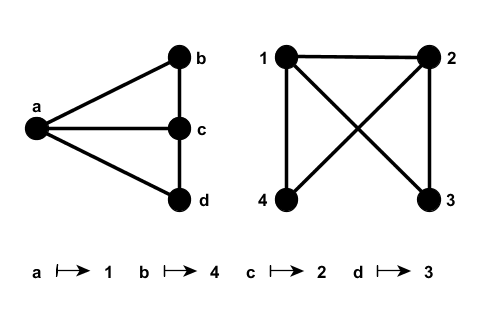
\includegraphics[width=\textwidth]{chapter1/fig/GI}
        \caption{Graph isomorphism}
        \label{fig:GI}
    \end{subfigure}
    ~
    \begin{subfigure}[b]{0.3\textwidth}
        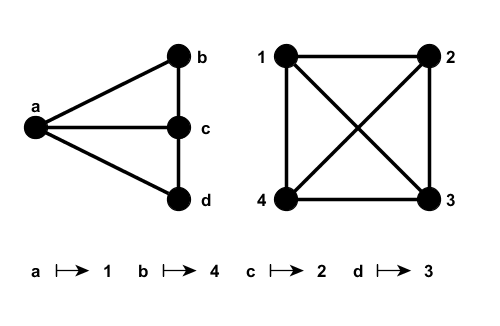
\includegraphics[width=\textwidth]{chapter1/fig/monomorphism}
        \caption{Graph monomorphism}
        \label{fig:monomorphism}
    \end{subfigure}
    ~
    \begin{subfigure}[b]{0.3\textwidth}
        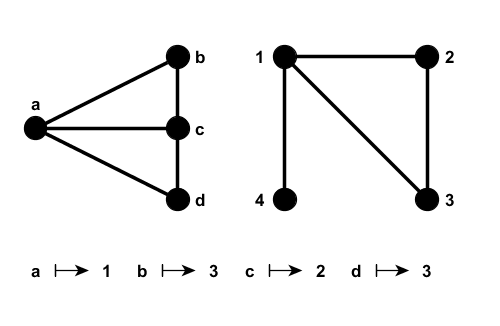
\includegraphics[width=\textwidth]{chapter1/fig/homomorphism}
        \caption{Graph homomorphism}
        \label{fig:homomorphism}
    \end{subfigure}
    \caption[Exact graph matching problems]{Exact graph matching problems}\label{fig:Exact_GM}
\end{figure}

%\subsection{Compexity}
All problems except graph isomorphism are proofed to be $NP-$complete~\cite{Garey_NPComplet}. This can be shown through a reduction of the respective matching problem to the clique problem. The graph isomorphism is currently shown to be in the class $NP$~\cite{Garey_NPComplet,Schoening_GI}. For some special types of graphs there exist however polynomial time algorithms (e.g. for %planar graphs~\cite{Hopcroft_Wong} and 
trees~\cite{Aho_Ullman, Garey_NPComplet}).

\ToDo{The exact graph matching problems are often too strict and intractable for the practical application and therefor do not lie in the focus of this work.} In following we describe several approaches for solving them.
% ---------------------------------------------------------------------------------------------------------------------------------
\section{Methods for solving exact graph matching problems}
The most used approach to solve an exact graph matching problem is based on a tree search with backtracking. This method starts with an empty set of correspondences and tries stepwise to expend it according to provided rules until a complete solution is found. Each partial solution represent a node of a search tree and all nested solutions build a branch in this tree. If it happens, that in some step a current set of correspondences cannot be expended further due to problem constraints, the current branch in the tree is cut. The method backtracks to the last feasible solution and tries to find another way to expend it further. The algorithms based on a tree search are very slow, if they need to traverse a whole tree. However, they can be speeded up by applying some heuristics to detect unpromising branches and exclude them from the search. The most known algorithm in this group, which uses depth-first-rule to traverse a tree, is the branch and bound algorithm~\cite{Reingold}.

The one of the first algorithms, that used the described technique, is the one by Ullman~\cite{Ullmann}. Later it was extended and improved mostly by the suggestion of a new pruning heuristics. A small comparison of different algorithms in this group with diverse heuristics is reported in~\cite{Lee2013}. We also want to mention here another well known algorithm on graphs, which uses the tree search method, namely the algorithm by Bron and Kerbosch~\cite{BronKerbosch} for finding cliques in an undirected graphs. The last problem closely related to the graph matching, as the maximal common subgraph problem can be reduced to the problem of finding the maximal clique~\ToDo{cite}.

From the other techniques we want to mention the algorithm described by MacKay~\cite{McKay}, which uses group theory to solve graph isomorphism problem, and an approach based on decision trees~\cite{Messmer1999,Shearer2001,Shearer1998} for matching graph ((sub)graph isomorphism) against a set of graphs.
% ---------------------------------------------------------------------------------------------------------------------------------
\section{Inexact graph matching}
As we mentioned above exact graph matching problems are often not applicable to real-world problems. There are two possible reasons for that. \ToDo{On the one hand, there are natural variations in the structure of graphs, that describe a same object}On the one hand, same object can be described by graphs with different structure. Those variations could be a consequence of object deformations or noise influence, that can occur in some real world applications. On the other hand, solving a graph matching problem exactly can be time and/or memory consuming. As a consequence one can be interested in solving graph matching problem inexactly. In this case, a strong edge preserving mapping between the nodes of two graphs is not required.

\vspace{-12pt}
\begin{figure}[htb]
	\centering
	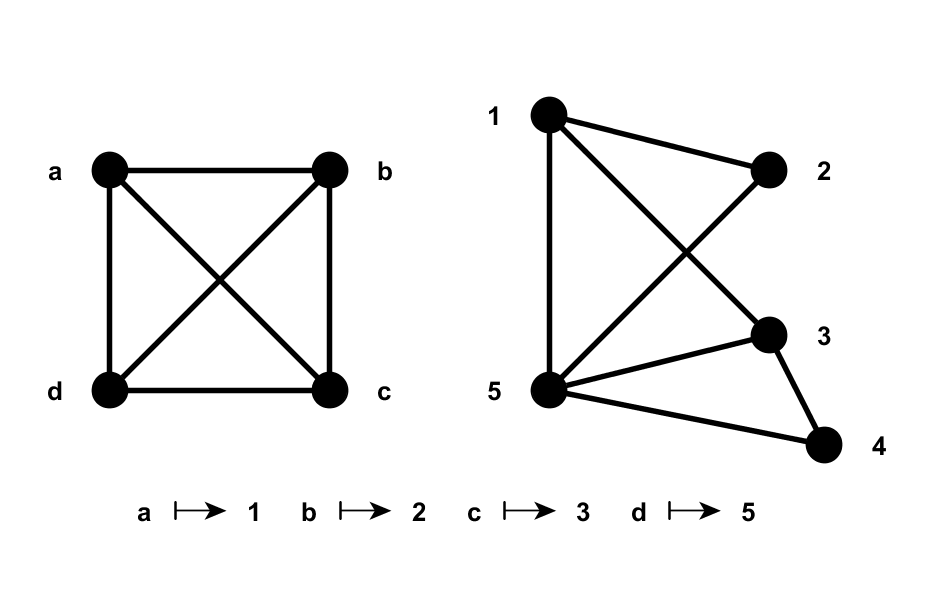
\includegraphics[width=0.5\textwidth]{chapter1/fig/inexactGM}
    \caption{Inexact graph matching}
    \label{fig:inexact_GM}
\end{figure}
\vspace{-10pt}
Let us recall the problem statement \eqref{gGMP}: 
\begin{equation*}
m = \argmax_{\hat{m}}S(G^I, G^J, \hat{m})
\end{equation*}
where $S(G^I, G^J, \hat{m})$ defines a similarity measure between the attributed graphs $G^I = (V^I, E^I,D^I)$ and $G^J = (V^J, E^J,D^J)$. The mapping $m$ is required to be total and sometimes also injective, to guarantee one-to-one matching.

Depending on the case, if an algorithm for solving problem~\eqref{gGMP} finds a global solution or not, this algorithm is called \emph{optimal} or~\emph{suboptimal}, respectively. The choice, which algorithm to select depends on a specific problem. It should be noted, that optimal inexact algorithms is not necessary faster than the exact one. On the other hand, suboptimal inexact algorithms often do not have any performance guarantee.

There are also different ways to define a similarity function $S(G^I,G^J,m)$, which leads to high number of different approaches inside the group of inexact graph matching algorithms. In the following section we summarized the most common forms of the objective function of the problem~\eqref{gGMP}.
% ---------------------------------------------------------------------------------------------------------------------------------
\subsection{Graph matching objective function}
In some literature (e.g.~\cite{Herault1990_SimulatedAnnealing,FastPFP,Lyzinski2015,Roth2001,Vogelstein_BrainGraphs,Zazlavskiy2008_PATH}) instead of defining a similarity function as it is done by Eq.~\eqref{gGMP} one speaks about dissimilarity between two graphs. The goal in this case is to minimize it. Two both formulations of the problem are however equivalent and one can easy transform one into other.
% ---------------------------------------------------------------------------------------------------------------------------------
\subsubsection{Quadratic Optimization Problem}
Let us consider two attributed graphs $G^I = (V^I, E^I,D^I)$ and $G^J = (V^J, E^J,D^J)$. We want to find a mapping $m$ between the nodes of this graphs. Let the size of the graphs be $n_1$ and $n_2$ respectively. Generally, $n_1$ and $n_2$ can be different, but then we assume without losing generality $n_1\le n_2$. Here and further, we require a mapping $m$ in \eqref{gGMP} to be total and injective, which guarantees, that each node of the first graph will be matched to exactly one node of the second graph (one-to-one matching). 

We start first with a even stricter assumption, that $n_1=n_2=n$ and the matching is bijective. In this case a mapping between nodes of two graphs defines a permutation $\sigma$ of the set $\{1,\dots,n\}$. Each permutation $\sigma$ can be represented by the permutation matrix $P=\{P_{ij}\}$, where
\begin{equation*}
P_{ij}=\begin{cases}
 1, & \text{if } \sigma(i)=j, \\
 0, & \text{otherwise.} \\
\end{cases}
\end{equation*}
We denote with $\Pi_n$ the set of all feasible permutations:
\begin{equation*}
\Pi_n=\{P\in\{0,1\}^{n\times n}|\sum_{i=1,\dots,n}P_{ij}=\sum_{j=1,\dots,n}P_{ij}=1\quad\forall i,j=1,\dots,n\}
\end{equation*}
Let matrices $A^I$ and $A^J$ be the adjacency matrices of the graphs $G^I$ and $G^J$ respectively. We assume, that in case of weighed graphs, the adjacency matrices contain edge weights, instead of binary values. We can now formulate the graph matching problem as~(compare with \cite{Herault1990_SimulatedAnnealing,FastPFP,Lyzinski2015,Roth2001,Umeyam1988,Zazlavskiy2008_PATH}):
\begin{equation} \label{eq:QAP1}
%P = \argmin_{\hat{P}\in\Pi_n}\|A^I\hat{P}-\hat{P}A^J\|^2
P = \argmin_{\hat{P}\in\Pi_n}\|A^I-\hat{P}A^J\hat{P}^T\|^2+\|D^I-\hat{P}D^J\|^2_2
\end{equation}
where $\|\cdot\|$ is the matrix Frobenius norm and $\|\cdot\|_2$ is Euclidean norm ($L^2$ norm). Some authors (e.g. Vogelstein et al. in~\cite{Vogelstein_BrainGraphs}) use slightly different, but equivalent reformulation of it, namely:
\begin{equation} \label{eq:QAP2}
P = \argmin_{\hat{P}\in\Pi_n}\|A^I\hat{P}-\hat{P}A^J\|^2+\|D^I-\hat{P}D^J\|^2,
\end{equation}
After some transformations, the problem \eqref{eq:QAP1} can be reformulated as~(see~\cite{Burkard98thequadratic}, Appendix~\ref{appendixA}):
\begin{equation} \label{eq:QAP3}
P = \argmin_{\hat{P}\in\Pi_n}\vec(\hat{P})^T(-(A^J)^T\otimes(A^I)^T)\vec(\hat{P})-\vec(D^I(D^J))^T\vec(\hat{P})
\end{equation}
where $\otimes$ denotes the Kronecker product and $\vec(\hat{P})$ is a column-wise vectorization of $\hat{P}\in\Pi_n$.

The minimization problem~\eqref{eq:QAP3} is the \emph{quadratic assignment problem}, which is know to be $NP-$hard~\cite{Burkard98thequadratic,Sahni1974}.

The both formulations~\eqref{eq:QAP1},~\eqref{eq:QAP3} have their advantages and disadvantages. The main benefit of \eqref{eq:QAP1} is the low space complexity $\mathcal O(n^2)$, where the space requirement of \eqref{eq:QAP3} estimates with $\mathcal O(n^4)$. This makes the second formulation to be tractable only for relative small graphs. The drawback of both formulations is the strict penalization function of edge disagreements, namely the squared Euclidean distance between matched edges. This follows straight forward from \eqref{eq:QAP1}. In this sense the last formulation can be easily generalized in the way, we represent below. 

We return back to the case where $n_1\not=n_2$. Let us denote with a binary vector $x\in \{0,1\}^{n_1n_2}$ the column-wise vectorization of the assignment matrix $P$, which is not necessary a permutation matrix anymore. It is obviously, that $x_{(j-1)n_1+i}=1$, if a node $v_i\in V^I$ is matched to a node $u_j\in V^J$, and $x_{(j-1)n_1+i}=0$ otherwise. For simplicity we will write further $x_{ij}$ instead of complicated form $x_{(j-1)n_1+i}$.
 
%For this, we also assume, that $|V^I|=n_1$, $|V^J|=n_2$ and $n_1$ is not necessary equal to $n_2$. The maximum number of possible matches is though equal to $\min(n_1, n_2)$.

To measure a similarity between graphs one considers two different kinds of similarities: second-order \emph{edge similarity} and first-order \emph{node similarity}. The first one is defined as a function of the edges $s_E:E^I\times E^J\rightarrow\mathbb{R}$ and should penalize a disagreements in the structure of two graphs. The second one $s_V:V^I\times V^J\rightarrow\mathbb{R}$ represent additional constraints on the possible node correspondences.

%Now we want to reformulate the objective function in \eqref{gGMP} using introduced node and edge similarity functions.
%A found mapping m (see Eq.~\eqref{gGMP}) gives us a set of node correspondences, which maximizes the similarity value between two graphs. Such a subset can be represented by a binary vector $x\in \{0,1\}^{n_1n_2}$, where $x_{(j-1)n_1+i}=1$, if node $v_i\in V^I$ is matched to node $u_j\in V^J$, and $x_{(j-1)n_1+i}=0$ otherwise. For simplicity we will write further $x_{ij}$ instead of $x_{(j-1)n_1+i}$.
%\footnote{Vector $x$ is a column wise vectorization of the correspondence matrix $X\in\{0,1\}^{n_1\times n_2}$, where $X_{ij}=1$, if the node $v_i\in V^I$ is matched to the node $v_j\in V^J$, and $0$ otherwise.}

Using the introduced notation and definitions of the node and edge similarity functions the function $S(G^I,G^J,m)$ in~\eqref{gGMP} can be now rewrite as follows:
\begin{equation}\label{eq:sumQAP}
	S(G^I,G^J,m)=\sum_{\substack{x_{ij}=1\\x_{i^\prime j^\prime}=1}}s_E(e_{ii^\prime},e_{jj^\prime}) + \sum_{x_{ij}=1}s_V(v_{i},v_{j})
\end{equation}
This formula can be also expressed in matrix form. We define an \emph{affinity} or \emph{similarity matrix} $S\in\mathbb{R}^{n_1n_2\times n_1n_2}$, whose diagonal elements are $s_V(v_i, u_j)$ and non-diagonal elements are $s_E(e_{ii\prime}, e_{jj\prime})$. Using this matrix we obtain the following formulation of the graph matching problem as an quadratic optimization problem \cite{Cho2014_Haystack, Cho2010_RRWM, Cho2012_ProgressiveGM, Conte2004,Rangarajan1996_GAGM,Leordeanu2005_SM,Leordeanu2009_IPFP}:
\begin{alignat}{2}
    &     && \argmax_x{x^TSx}                           \label{eq:gQAP1}\\ %\notag\\
    & \text{s.t. } &&  x\in \{0,1\}^{n_1n_2}            \label{eq:gQAP2}\\
    &             &&  \sum_{i=1\dots n_1} x_{ij}\le 1    \label{eq:gQAP3}\\
    &             &&  \sum_{j=1\dots n_2} x_{ij}\le 1    \label{eq:gQAP4}
\end{alignat}
We notice, that in the case, where $n_1=n_2$, both conditions (\ref{eq:gQAP3}) and (\ref{eq:gQAP4}) will be fulfilled with equality. We call this constraints~\emph{two-way constraints}~\cite{Rangarajan1996_GAGM}, as they enforce one-to-one matching .

One can easily see, that the formulation \eqref{eq:gQAP1}-\eqref{eq:gQAP4} can be obtained from \eqref{eq:QAP3} by setting $S=(A^J)^T\otimes(A^I)^T$ with diagonal elements equal to $\vec(D^I(D^J)^T)$.
%A Quadratic Optimization Problem is known to be \emph{NP}-hard \cite{Sahni1974}. This limits greatly the size of a graph, for which a exact solution can be calculated in reasonable time. Due to this there are a number of algorithms \cite{Cho2014_Haystack, Cho2010_RRWM, Cho2012_ProgressiveGM, Chui2003, Suh_CVPR2015}, that solve graph matching problem inexact.

Below we list a different ways to define a node and edge similarities between two attributed graphs we found in the literature.

%\subsubsection{Edge similarity}
\textbf{Edge similarity}

One possible approach to calculate an edge similarity is to calculate \emph{edge dissimilarity} $d_E:E^I\times E^J\rightarrow\mathbb{R}$ first and then transform it into similarity by using, for example, one of the following functions~\cite{Cho2014_Haystack, Cho2009_AgglClustering, Cho2010_RRWM,Cho2012_ProgressiveGM}:
\begin{itemize}
	\item \itemEq{s_E(e_{ii\prime}, e_{jj\prime})= exp(-\frac{d_E(e_{ii\prime}, e_{jj\prime})^2}{\sigma^2_{s}}) \label{eq:edge_sim1}}
	\item \itemEq{s_E(e_{ii\prime}, e_{jj\prime})= \max(\beta - d_E(e_{ii\prime}, e_{jj\prime})/\sigma^2_{s},0)  \label{eq:edge_sim2}}
\end{itemize}
where $e_{ii\prime}\in E^I$ and $e_{jj\prime}\in E^J$. The parameters $\sigma_s$ and $\beta$ define a sensibility of a graph matching algorithm to the dissimilarities between the graphs.

This leads us to the question how to calculate edge dissimilarity. The most obvious way is to compare a weights of the edges, if they are provided. An other alternative could be to use length of the edges~\cite{Cho2014_Haystack, Cho2009_AgglClustering, Cho2010_RRWM,Cho2012_ProgressiveGM}, if coordinates of the nodes in some system (usually, Cartesian coordinates) are known. It is a significant assumptions, which holds however for almost all graphs arose in practical application.

Sometime a node attributes can be used to calculate edge dissimilarities. For example, if graph nodes are described by an ellipse with known center coordinates and orientation one can calculate so-called geometric dissimilarity of the edges~\cite{Cho2009_AgglClustering,Cho2012_ProgressiveGM}:
\begin{alignat}{4}\label{eq:geomDiss}
& d(e_{ij},e_{i^\prime j^\prime}) && =\frac{1}{2}(d_{geo}(m_j|m_i) && +d_{geo}(m_i|m_j)) \\
& d_{geo}(m_j|m_i) && =\frac{1}{2}(\|x_{j^\prime}-H_{i}x_j\| && + \|x_{j}-H^{-1}_ix_{j^\prime}\|) \\
& d_{geo}(m_i|m_j) && =\frac{1}{2}(\|x_{i^\prime}-H_{j}x_i\| && + \|x_{i}-H^{-1}_{j}x_{i^\prime}\|) 
\end{alignat}
where $m_i$ is a correspondence between nodes $v_i$ and $v_{i^\prime}$ and $H_i$ is an affine homography from $v_i$ to $v_{i^\prime}$ estimated based on elliptic regions around each node.

An another way to calculate edge similarities could be to use directly some similarity measure, such as ~\ToDo{cosine similarity}.

\textbf{Node similarity}

%\subsubsection{Node similarity}
If a given graphs have node attributes, the most natural method to measure a similarity of two nodes is to compare their attributes. In the most of the seen literature, the node attributes are represented by a $k-$dimensional real vectors: $D^i,D^J\subset\mathbb{R}^k$. This means, we can adopt all techniques\footnote{with exception of the geometric dissimilarity measure} described in previous paragraph to define a node similarity function. Additionally, in case when node attributes can be considered as some distribution (e.g. distribution of gray values of an image around a node), one can use metrics to measure distance between two distributions. For example, Schellewald and Schn\"orr~\cite{Schellewald2005} used the earth mover's distance for this purpose.
% ---------------------------------------------------------------------------------------------------------------------------------
\subsubsection{Error correcting graph matching}
Another way to measure the similarity between two graphs is based on a \emph{graph edit distance}~\cite{Bunke1983_inexactGM}. The graph edit distance is defined through costs of \emph{graph edit operations}, that transform on graph into another. Those operations are insertion, deletion and substitution of nodes and edges of a graph. An algorithm, that uses graph edit distance for graph matching, is often called~\emph{error correcting}~\cite{Conte2004}.

Consider two attributed graphs $G^I = (V^I, E^I,D^I)$ and $G^J = (V^J, E^J,D^J)$ and matching $m$ between subsets $\bar{V}^I,\bar{V}^J$ of $V^I$ and $V^J$ respectively. The edit operations on nodes can be directly defined by the mapping $m$~\cite{Bunke1998_ErrTolerantGM}:
\begin{itemize}
	\item if $m(v_i)=v_j$ for $v_i\in\bar{V}^I,v_j\in\bar{V}^J$, then a node $v_i$ is \emph{substituted} by a node $v_j$
	\item nodes in $V^I\backslash\bar{V}^I$ are \emph{deleted}
	\item nodes in $V^J\backslash\bar{V}^J$ are \emph{inserted}.
\end{itemize}
An edit operation of an edge is defined based on a transformations applied to its end nodes. For example, insertion of a node $v_j\in V^J$ implies that all edges, connected to this node, are also inserted. Alternatively, if a node $v_i\in V^I$ is deleted, then all edges incident to this node are also deleted. We say, that an edge $\{v_i,v_{i^\prime}\}\in E^I$ was substituted by an edge $\{v_j,v_{j^\prime}\}\in E^J$, if the nodes $v_i,v_{i^\prime}$ were mapped in $v_j,v_{j^\prime}$.

We assume that all operations can be performed simultaneously. Let $S=\{s_1,s_2,\dots,\newline s_k\}$ denote a set of operations needed to transform the graph $G^I$ into the graph $G^J$. 
Each edit operation $s_i, 1\le i\le k,$ has an assigned nonnegative cost $c(s_i)$. The cost of the whole sequence $S$ is defined then as $\sum_{i=1}^{k}c(s_i)$. Using it and following papers~\cite{Bunke1983_inexactGM, Wang1995} we define a \emph{edit distance} between the graphs $G^I$ and $G^J$ as follows:
\begin{eqnarray} \label{eq:editDist}
dist(G^I,G^J,m) = \min\limits_{S=\{s_1,\dots,s_k\}}c(S)
\end{eqnarray}
The task of the error-corrected graph matching is to find such a mapping $m$ between $V^I$ and $V^J$, which induces a cheapest transformation between the graphs.

The cost functions of each operation are often defined as a functions of edge weights and node attributes. Their exact definitions depend however on a specific application. Sometimes, it can be helpful, when the distance measure~\eqref{eq:editDist} defines a metric, which is not automatically the case. Bunke and Allermann~\cite{Bunke1983_inexactGM} have shown that the graph edit distance can fulfill the properties of a metric under a specific conditions on the cost functions of the individual edit operations. For example, one of this conditions is, that a single operation is always preferred to a sequence of two operations with the same result (triangular inequality of the operation cost functions). Later, Bunke and Shearer~\cite{Bunke1998_graphDist} suggest a new graph edit distance, that does not depend on the cost of the edit operations, and is a metric.

An interesting question is, how does the error corrected graph matching problem correspond to the other matching problems defined previously. It was shown in~\cite{Bunke1999_UnderlyingCosts}, that graph isomorphism, subgraph isomorphism and maximum common subgraph problems can be considered as a special cases of the error correcting graph matching. The same holds for the inexact graph matching problem formulated as in~\eqref{eq:QAP1}. This is easy to see, if one rewrite the objective function of ~\eqref{eq:QAP1} as $\sum_{i=1}^n\sum_{j=1}^{n}(A^I_{ii^\prime}-A^J_{\sigma(i)\sigma(i^\prime)})^2$. Comparison of this expression with the definition of $c(S)$ in~\eqref{eq:editDist} leads us direct to the idea, how to set the edge insertion/deletion/substitution cost functions so as to make the problem formulations equivalent: 
\begin{equation*}
c(e_{\text{subst}})=(A^I_{ii^\prime}-A^J_{\sigma(i)\sigma(i^\prime)})^2\quad c(e_{\text{insert}})=(A^J_{\sigma(i)\sigma(i^\prime)})^2\quad c(e_{\text{del}})=(A^I_{ii^\prime})^2
\end{equation*}
% ---------------------------------------------------------------------------------------------------------------------------------
\section{Methods for solving inexact graph matching problems}
In following we briefly describe a common approaches for solving inexact graph matching problems in field of Computer Vision and Pattern Recognition. We subdivided them into groups based on their main idea.
% ---------------------------------------------------------------------------------------------------------------------------------
\subsection{Discrete optimization}
\subsubsection{Tree search methods}
Similar to the exact graph matching problems a tree based methods with backtracking were successfully applied to solve inexact matching problems. They were especially wide used for the error-correcting graph matching. In this case a searching procedure can be efficiently guided, so that the required time is shorter than exponential time, which is needed by a blind searching. This can be done by defining the score of the tree nodes as a sum of two scores: a matching score of a current partial solution and a heuristically estimated score of a remaining nodes. The algorithms in this group differ mainly in a suggested heuristics for calculation of future costs and in rules for tree traversing. The most used strategies for tree traversing are depth-first-search~\cite{Cormen} and $A^*$-Algorithm~\cite{AStar}.

One of the first algorithms for inexact graph matching based on the three search was presented by Tsai and Fu in paper~\cite{Fu1979}. It is an optimal inexact graph matching algorithm. For further examples of the tree search methods for inexact graph matching we refer to papers \cite{Bunke1983_inexactGM,Shapiro1981,Wang1995}.
\subsubsection{Simulated Annealing}
Simulated annealing is a heuristic for searching the global optimum of a given energy function~\cite{Burkard98thequadratic}. It is an extension of the Metropolis Algorithm~\cite{Metropolis}, that was suggested for finding an equilibrium of a physical system consisting of individual particles by heating it first and then cooling it slowly down. Speaking in terms of a graph matching problem its solutions define states of a system and corresponding objective scores its energy. The idea is to find a state with the lowest energy by performing some random changes in a system. This can be a random exchange of correspondences between two pairs of matched nodes. A change, that decreases the total dissimilarity of graphs, is always accepted. On the other side, a change, that increases energy function, is accepted with some probability. This probability and number of changes per iteration is controlled by the temperature parameter $T$. The lower $T$ the fewer changes are allowed and the lower the accepted probability is. 

The application of the simulated annealing to the graph matching problems can be found in paper~\cite{Herault1990_SimulatedAnnealing}. This heuristic can also be used to solve a quadratic assignment problem~\cite{Burkard98thequadratic}.
% ---------------------------------------------------------------------------------------------------------------------------------
\subsection{Continuous optimization}
This group of methods is one of the biggest and deep investigated. The main idea is to transform the inexact graph matching problem into a continuous optimization problem. This can be done, for example by relaxing the integer constraints in the discrete optimization problems~\eqref{eq:QAP1},~\eqref{eq:gQAP1}. A found solution must be converted afterwards back in the discrete domain. Depending on techniques applied to solve a continuous problem we subdivide this group into several subgroups. The list of the algorithms, presented here, is not complete. As we already mentioned, we selected mainly the classical approaches and/or those we investigated during the work on this thesis.

The first subgroup of the algorithms contains the algorithms, that relax all constraints of a graph matching problem, find a continuous solution of the new nonlinear problem and project it back into discrete domain. 

In 1996 Gold and Rangarajan presented a graduated assignment algorithm for graph matching (GAGM)~\cite{Rangarajan1996_GAGM}. It is an iterative algorithm, which uses \emph{deterministic annealing}\footnote{Deterministic annealing is similar to the simulated annealing, but uses deterministic techniques to find a minimum of an energy function by a current value of a temperature parameter~\cite{Rose1991_DA}.} to solve the graph matching problem formulated as~\eqref{eq:gQAP1}. The authors use Taylor series approximation to relax the initial quadratic assignment problem to linear assignment problem. The two-way constraints are enforced at each iteration by converting a  found continuous solution into a double stochastic matrix by applying exponentiation and Sinkhorn normalization~\cite{Sinkhorn1964}. This technique is called \emph{soft-assign}. The deterministic annealing was also used in~\cite{Rangarajan96_LagRelax} to solver Lagrangian Relaxation of the problem~\eqref{eq:QAP1} and in the robust point matching algorithm with thin-plane spline (RPM-TPS)~\cite{Chui2003}. The solution obtained by this method is however not necessary optimal and the behavior of the algorithms depends highly on the selected parameters, especially those, which control the annealing schema.

Another iterative algorithm was proposed in paper~\cite{Leordeanu2009_IPFP} and is called an integer projected fixed point method (IPFP). It consists of two steps, which we shortly describe below. In the first step, an initial solution has to be chosen. It can be, for example, a continuous or discrete solution obtained by some other algorithm. The second step iteratively improves this solution by applying \emph{Frank-Wolfe algorithm}~\cite{Wolfe1956} adapted to the graph matching problem. This algorithm finds first the best search direction by solving an linear assignment problem. The last arises as in GAGM by the maximization the first-order Tailor series approximation of the objective function. The maximization is performed in the discrete domain using the Hungarian algorithm~\cite{Kuhn1955}. Then the initial objective function is further maximized in a continuous domain along found direction. The authors show, that in the praxis IPFP tends to converge towards discrete solutions, that are close to the optimum.

The Fast Approximative Quadratic Programming Algorithm (FAQ), presented in~\cite{Vogelstein_BrainGraphs}, also uses Frank-Wolfe algorithm to solve a continuous relaxation of the problem~\eqref{eq:QAP2}. However FAQ performs completely in a continuous domain and has the third step, which maps a found continuous solution back onto discrete domain. Unlike IPFP, the FAQ algorithm do not use the similarity matrix $S$. This gives it a big advantage of the less space requirement, which make it possible to apply the algorithm to graphs of a big size\footnote{Evaluation results in the paper include test with a graphs with up to $1000$ nodes}. 

Another approach, that uses Frank-Wolfe algorithm, is the PATH-Algorithm~\cite{Zaslavskiy2010}. The algorithms finds first the global optimum of the Lagrangian relaxation of the problem~\eqref{eq:QAP2}. This is done by applying the Newton method~\cite{Book_ConvOpt}. Afterwards the found solution is projected back onto discrete domain by solving a sequence of convex and concave problems, which are solved by Frank-Wolfe algorithm.

The fast projected fixed-point algorithm (FastPFP) proposed by Lu et al.~\cite{FastPFP} is very close to IPFP. This algorithm uses \emph{projected fix point method} to find a solution of a continuous relaxation of the problem~\eqref{eq:QAP1}. Compared to IPFP the new algorithm uses projections onto a continuous domain, instead of discrete. Furthermore the authors proofed the linear convergence rate of their algorithm, whereby the convergence rate of IPFP is unknown. The FastPFP, similar to FAQ, does not have a memory issues because it does not use a similarity matrix $S$ and is generally faster than both IPFP and FAQ, because it does not solve a linear assignment problem on each iteration.

A completely different approach to solve graph matching problem was suggested by Schellewald and Schn\"orr~\cite{Schellewald2005}. They formulated graph matching problem as a regularized bipartite matching problem~\cite{Diestel2000}, which is then relaxed to a convex semidefinite program. The last can be solved with standard algorithms, such as the interior point method~\cite{Book_ConvOpt}. A novelty of the algorithm consists in a probabilistic post-processing step, which convert a found continuous solution  into discrete one. The suggested algorithm is easy to apply, as it has only one parameter. However the considered relaxation problem has a squared size comparing to initial problem~\cite{Cour2006}. Consequently, the algorithm is not suitable for big graphs.
% ---------------------------------------------------------------------------------------------------------------------------------
\subsubsection{Spectral methods}
A big group of algorithms for solving graph matching problems is built by those, which use an eigenvalue decomposition~\cite{Book_ConvOpt} of the adjacency matrices of given graphs. The idea behind this is, that the eigenvalues of the adjacency matrices of two isomorphic graphs are equal, because they are invariant to the node permutation\footnote{Indeed, let $A$ and $B$ be adjacency matrices of two isomorphic graphs. That means, that $B=PAP^T$, where $P$ is a permutation matrix. If $\alpha$ is an eigenvalue of $A$: $Av=\alpha v$ and $u=Pv$, then the following holds $Bu=(PAP^T)u=(PA)(P^Tu)=(PA)v=P(\alpha v)=\alpha u$. So $\alpha$ is an eigenvalue of $B$}.

One of the first algorithms, which uses spectral techniques, is the one by Umeyama\newline~\cite{Umeyam1988}. He considers the case, when two graphs have the same number of nodes and matching between them is bijective. This means, that a desired correspondence matrix must be a permutation matrix. The author proofs, that an orthogonal matrix, which minimizes the objective function of~\eqref{eq:QAP1}, can be formulated based on the eigenvalue decomposition of the adjacency matrices of given graphs. The terms of this formulation are used to define a linear assignment problem, whose solution is a solution of the initial problem. In case, when given graphs are sufficiently close, those solution is optimal or nearly optimal.

We also want mention, that this algorithm is highly limited in its application due to its requirements. We also want to mention, that it works only with graph geometry and does not consider attributes of nodes and edges.

The more resent algorithm is from this group of methods is called spectral matching (SM)~\cite{Leordeanu2005_SM}. The algorithm works with the general formulation~\eqref{eq:gQAP1}. It relaxes both two-way and integer constraints~\eqref{eq:gQAP2}-\eqref{eq:gQAP4} and obtain the optimal solution of this relaxation by taken the principal eigenvector of the matrix $S$. This is done by using \emph{the power iteration method}~\cite{PowerIteration}. The found continuous solution is binarized by applying a simple greedy heuristic, that enforces previously relaxed matching constraints.

A generalization of the SM algorithm is proposed in~\cite{Duchenne2011}. The authors suggest to consider similarities between tuples of nodes and not only pairs to improve graph matching quality. They formulate a new problem using hyper-graphs and tensor notation. The solution strategy is however the same, as it is in~\cite{Leordeanu2005_SM}: the solution is approximated with the principal eigenvector of the matrix $S$ and discretized afterwards. However, the power iteration method should be adopted to the tensor based problem, because it cannot be applied directly.

Before going to the next section we want shortly describe a max-pooling approach by Cho and Duchenne~\cite{Cho2014_Haystack}, which uses ideas similar to both GAGM~\cite{Rangarajan1996_GAGM} and SM~\cite{Leordeanu2005_SM}, but replaces one of the sum in a updating step with maximum-operation. The algorithm solves the graph matching problem formulation~\eqref{eq:gQAP1} by relaxing its integer constraints and omitting sum constraints. To approximate a solution of $\argmax_{x}x^TSx$ the max-pooling algorithm similar to GAGM uses first order Taylor expansion of the objective function. The maximization of the Taylor approximation can be done by the power method as it is done in SM.
The resulting update formula of the correspondence $(v_i,v_j),v_i\in V^I,v_j\in V^J$ has the form:
\begin{equation}
(Ax)_{ij}=x_{ij}s_V(v_i,v_{j})+\sum_{i^\prime\in N_i}\sum_{j^\prime\in N_j}x_{i^\prime j^\prime}s_E(e_{ii^\prime},e_{jj^\prime}),
\end{equation}
where $N_i$ denotes a direct neighborhood of a node $v_i$, i.e. set of its adjacent nodes.
The max-poling algorithm uses a maximum function instead of the second sum in the second term, which leads to
\begin{equation}
(Ax)_{ij}=x_{ij}s_V(v_i,v_{j})+\sum_{i^\prime\in N_i}\max_{j^\prime\in N_j}x_{i^\prime j^\prime}s_E(e_{ii^\prime},e_{jj^\prime}).
\end{equation}
This simple idea helps to suppress a noisy entries of the outlier matches, because the last have more likely low similarity values. The proposed algorithm shows very good results in presents of numerous outliers, although there is no theoretical justification of its convergence.
% ---------------------------------------------------------------------------------------------------------------------------------
\subsubsection{Probabilistic frameworks}
Another group of algorithms applies \emph{relaxation labeling} to solve graph matching problem. The aim of the relaxation labeling is to find an optimal assignment between set of labels and set of objects. Each label has some initial probability to be assign to certain object. Those probabilities are set based on some informations known about the objects. In terms of graph matching problem, nodes of a one graph are considered as objects and nodes of another graph as labels. Initial probabilities of assignments between the nodes are calculated  based on the node and edge attributes. 

The earlier works on this formulation are the one by Fischer and Elschlager~\cite{Fischler1973} and Rosenfeld et al.~\cite{Rosenfeld1976}. In both cases, proposed algorithms start with some initial label probabilities and try to reduce a labeling ambiguities at each iteration based on labels of neighboring nodes. The process runs till convergence or some predefined number of iterations. The algorithms are heuristic, but reduce the complexity of the initial problem to polynomial~\cite{Christmas1995}.

A first algorithm with theoretically proofed update rule is suggested by Kittler and Handcock~\cite{Hancock_Kittler}. This was later improved by Christmas at al.~\cite{Christmas1995}, who suggested a method to included provided node attributes and edge weights into update rule of the labeling probabilities and not only in the initialization step.

Later algorithms formulate graph matching problem as Maximum A Posteriori probability~(MAP) estimation. For example, the matching process in paper~\cite{Hancock_StrucMatch} is a process of node exclusion and insertion, so that MAP rate monotonically increases in each iteration. This technique is suggested to effectively cope with the possible outliers in the sets of graph nodes. A node is considered as an outlier, if its deletion improves the consistency in the structure of two graphs. The structural constraints hereby are defined by a dictionary of feasible mappings between local neighborhoods (super-cliques) of nodes of two graphs. The algorithm shows good results in case of big number of outliers. It is however slow.

Another interesting idea is presented in paper~\cite{Hancock_EM_SVD}. Given two graphs, nodes of the first graph are considered as an observed data and the nodes of the other as hidden random variables. In this formulation the graph matching problem is solved using~\emph{Expectation-Maximization algorithm} (EM)~\cite{EM_Dempster1977}. A similar algorithm is presented in the resent paper~\cite{Sanrom2012}. However, it works with the continuous correspondences between the graph nodes and projects them in the discrete domain using soft-assign technique described previously. It also includes structural information\footnote{Structural relations between nodes are given through adjacency matrix of a graph. Geometrical relations are represented as relative position of the nodes with respect to each other~\cite{Sanrom2012}.} into matching process, whereby the algorithm from~\cite{Hancock_EM_SVD} uses only geometrical information. Both algorithm are however not applicable to a big graphs due to unlimited increasing of the formulated density function with the size of a graphs~\cite{Armiti2014}. A new scalable graph matching algorithm, which also uses EM to solve the problem formulated in a maximum likelihood estimation framework, is presented recently in~\cite{Armiti2014}. The scalability is achieved there by including information about already known correspondence into calculation of the density function.
% ---------------------------------------------------------------------------------------------------------------------------------
\subsubsection{Methods using clustering techniques}
We want \ToDo{place special separated emphasis to}to emphasize independently the methods, that use clustering techniques to improve the graph matching score or performance.

Minsu Cho~\cite{Cho2009_AgglClustering} proposes to use \emph{agglomerative clustering} on a set of candidate matches to effectively cop with outliers. The problem is formulates as in~\eqref{eq:gQAP1}. The considered graphs are attributed, so that candidate matches are selected based on the distance between node attributes. The algorithm is controlled by the dissimilarity measure between two clusters, which is defined as the average of $k$ smallest pairwise dissimilarities between points in two clusters. This linkage model is called by the authors \emph{adaptive partial linkage model}. Notice, that the points in clusters are pairwise correspondences between graph nodes. The dissimilarity between two nodes is defined as a linear combination of the node attribute dissimilarities and 
geometric dissimilarities defined as~\eqref{eq:geomDiss}. Empirical results show, that correct correspondences tend to build bigger clusters. In contrast to that, the outliers are likely to stay in small groups, so it possible to detect them using threshold value of the cluster size.

Another algorithm based on the hierarchical clustering is suggested by Carcassoni and Hancock~\cite{Hancock_ModalClusters}. Its main idea is to provide additional constraints, that can be used to improve the robustness of a graph matching algorithm against graph deformations. This was successfully achieved by using spectral methods to build the clusters. The $S$ eigenvectors associated with the first $S$ largest eigenvalues are selected as a cluster centers. After performing the clustering, a probabilistic matching algorithm is applied to match first the clusters and then the nodes inside the clusters.

Further benefit of using clustering methods lies in the potential complexity reduction. 
The first idea to achieve this is based on a hierarchical graph matching and appears, for example, in the work by Qui and Handcock~\cite{Hancock_GM_SpectralPart}. They suggest to use graph partition to create a new simplified graph, whose nodes represent clusters of initial graph. After partitioning graphs are matched in a similar manner as it is suggested by Carcassoni and Hancock~\cite{Hancock_ModalClusters}, where the derived clusters tie matching constraints. The used partition method is based on a spectral method and creates a set of non-overlapping node neighborhoods\footnote{A node neighborhood is defined here as a node with all its adjacent nodes.}. To build those they use Fiedler vector (eigenvector associated with the second smallest eigenvalue of a graph Laplacian matrix, see~\cite{Fiedler1975}). The authors provide a study, which shows that the matching with proposed partition technique is stable under structural errors. Additionally, they show, that the simplified graphs preserve structure of initial graphs. The last is shown by performing clustering of a group of different graphs before and after simplification.

The second idea to reduce complexity of the initial matching problem uses graph clustering to create a set of independent subproblems. The matching is then performed for each subproblem independently and due to reduced problem size faster. A solution of the whole problem is then obtained by combining local solutions. The great benefit of such approach is the ability to parallelize the computation process, which can lead to the significant time reduction.

The described idea is followed by Lyzinski et al. in their resent paper~\cite{Lyzinski2015}. The aim of the authors is to parallelize a graph matching algorithm for matching very big graphs. However the problem, they consider, is semi-supervised, what means that correct correspondences between some nodes are known. It is obvious, that the matching results of the subdivided problem depends highly on the quality of the graph clusters and established correspondences between the clusters of two graphs. In a perfect clustering, node that should be matched, must lie in the corresponding subgraphs. To ensure that the clustering is sufficiently good, the authors propose a technique, that first spectrally embeds graphs and then jointly cluster them. The algorithm was successfully applied to the graphs with $20000-30000$ nodes.

%\subsubsection{Resent algorithms for big graphs}
% ---------------------------------------------------------------------------------------------------------------------------------
\section{Graph matching algorithms studied in this thesis}
In this section we want for completeness describe in details graph matching algorithm used in our framework for graph matching. However, we do not provide theoretical justification of the algorithm steps and refer a reader to the original paper for that. We use the notation introduced above at the beginning of this chapter.

\subsection{Reweighted random walks for graph matching (RRWM)}
The presented here algorithm is developed by Minsu Cho et al.~\cite{Cho2010_RRWM} and interprets the graph matching problem~\eqref{eq:gQAP1}:
\begin{alignat*}{2}
    &     && \argmax_x{x^TSx}                           \tag{\ref{eq:gQAP1}}\\
    & \text{s.t. } &&  x\in \{0,1\}^{n_1n_2}            \tag{\ref{eq:gQAP2}}\\
    &             &&  \sum_{i=1\dots n_1} x_{ij}\le 1   \tag{\ref{eq:gQAP3}}\\
    &             &&  \sum_{j=1\dots n_2} x_{ij}\le 1   \tag{\ref{eq:gQAP4}}
\end{alignat*}
between two graphs $G^I=(V^I,E^I,D^I)$, $G^I=(V^I,E^I,D^I)$ in a random walk view. Authors define an association graph $G^{rw}=(V^{rw},E^{rw},D^{rw})$ based on the affinity matrix $S$. The set of nodes $V^{rw}$ of the new graph is represented by all possible correspondences between nodes in $V^I$ and $V^J$. This means, that $|V^{rw}|=n_1n_2$, where $|V^I|=n_1$ and $|V^J|=n_2$. We refer to a node of the graph $G^{rw}$ as $v_{ij}$ if it represent a correspondence pair $(v_i,v_j)$, $v_i\in V^I,v_j\in V^J$. The entry $S_{ij,i^\prime j^\prime}$ of the matrix $S$ defines the weight of the edge $\{v_{ij},v_{i^\prime j^\prime}\}\in E^{rw}$. We denote the weighted adjacency matrix of the graph $G^{rm}$ as $W$. An example of the construction is illustrated on the figure~\ref{fig:RRWM1},\ref{fig:RRWM2} below. Note, that we omitted contradiction edges, whose weights are equal zero, e.g. $\{a1,b1\}$.

%\vspace{-30pt}
\begin{figure}[h] %\label{fig:RRWM} 
	\centering
    \begin{subfigure}[b]{0.33\textwidth}
        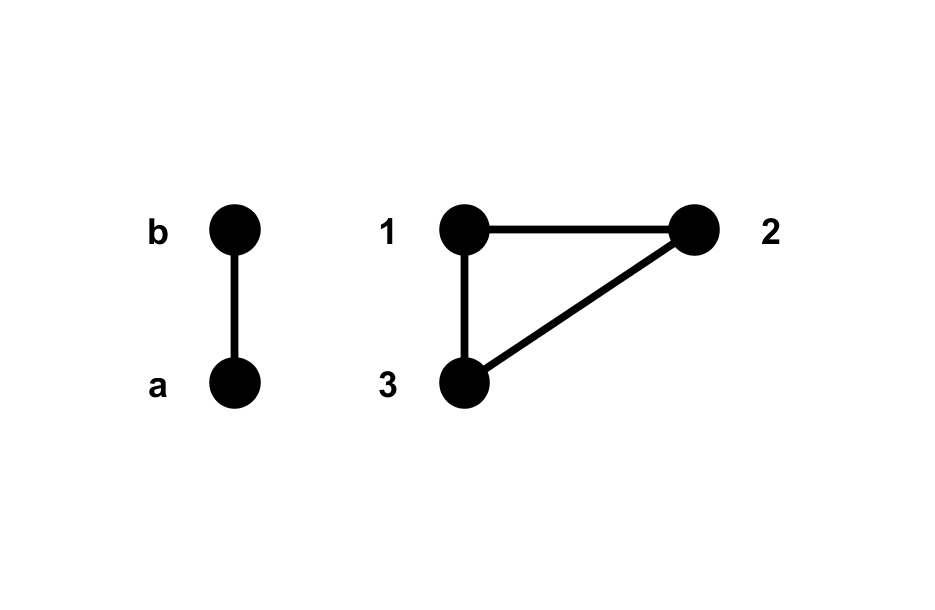
\includegraphics[width=\textwidth]{chapter1/fig/RRWM1}
        \caption{Two graphs to match}
        \label{fig:RRWM1} 
    \end{subfigure}
    ~
    \begin{subfigure}[b]{0.33\textwidth}
        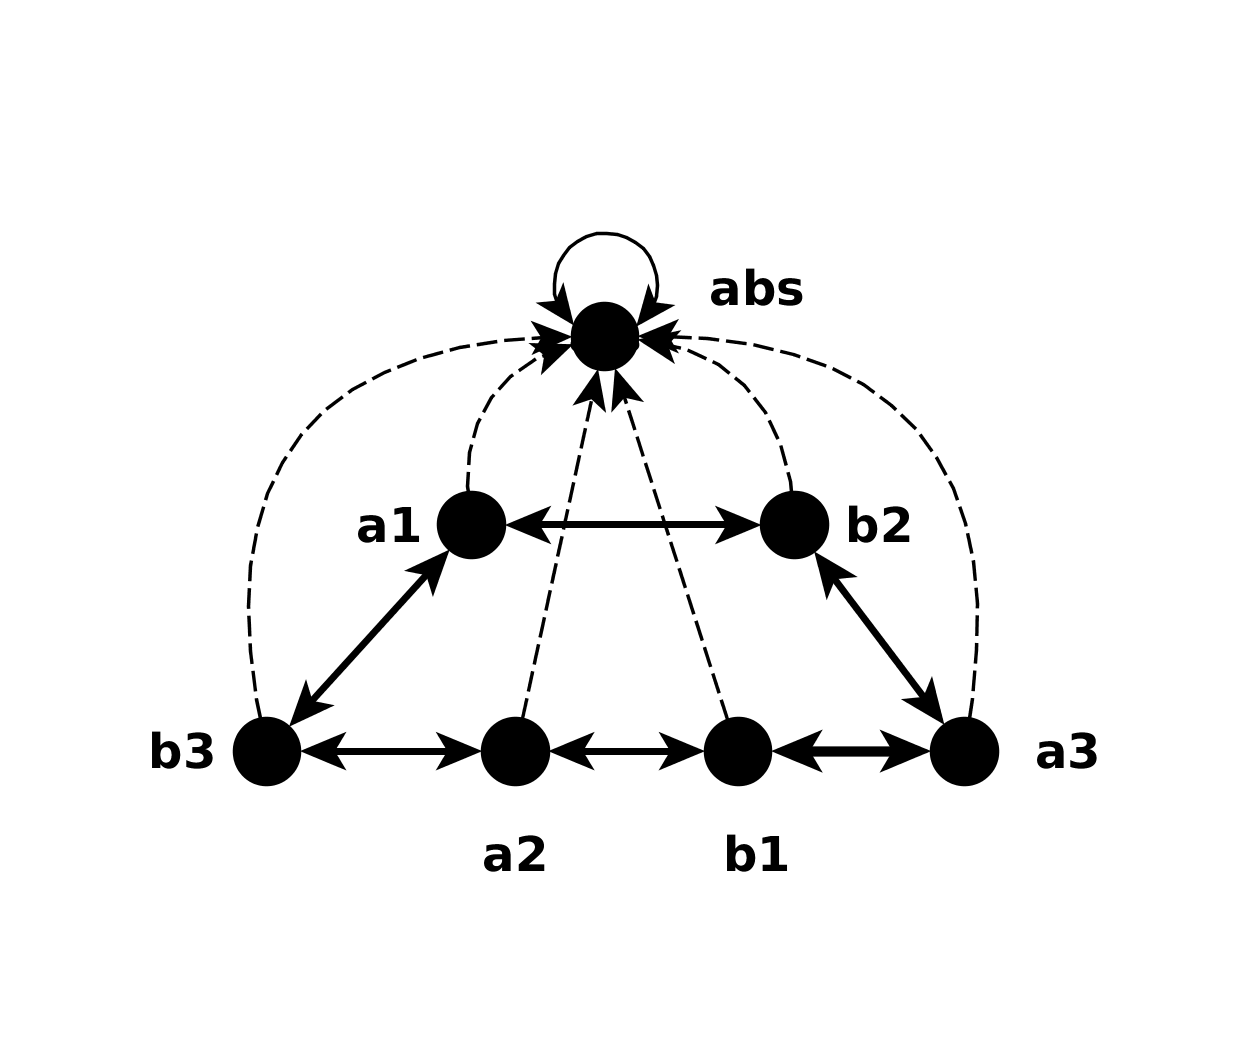
\includegraphics[width=\textwidth]{chapter1/fig/RRWM2}
        \caption{Association graph}
        \label{fig:RRWM2} 
    \end{subfigure}   
\caption{Association Graph of two given graphs for Reweighted Random Walk Method (compare with~\cite{Cho2010_RRWM})}
\end{figure}
%\vspace{-10pt}
It is obvious, that the graph matching problem between two graphs $G^I$ and $G^J$ is equivalent to finding a subset of nodes in the associated graph $G^{rw}$, so that the respective node correspondences between $V^I$ and $V^J$ satisfy matching criteria of the initial problem.
For finding such a subset the authors adopt the page ranking algorithm based on a random walk, which is assumed to be a Markov chain~\cite{PageRank}. To describe a Markov chain one defines a transition matrix $P$. An usual approach to define a transition matrix of a wighted graph $G^{rw}$ is to convert the weighted adjacency matrix $W$ of the graph into a stochastic matrix by the following normalization $P=D^{-1}W$, where $D$ is a diagonal matrix with entries $D_{kk}=\sum_{l}{W_{kl}}$. This method was, for example, used in PageRank algorithm~\cite{PageRank}. It is however not suitable for the graph matching purposes, because it treats false correspondences equal to all other correspondences. To avoid this problem Cho et al. introduce an additional absorbing node $v_{abs}$~(see Fig.~\ref{fig:RRWM2}) in the Graph $G^{rw}$. This node represents a state, that can be reached from each node $v_k=v_{ij}\in V^{rw}$ with the probability $1-D_{kk}/D_{\text{max}}, D_{\text{max}}=max_{k}D_{kk}$, but can not be left any more. Using $D_\text{max}$ the matrix $W$ is converted into a stochastic matrix by its multiplication with the factor $1/D_{\text{max}}$.
Summarizing, the transition matrix $P\in\mathbb{R}^{(n_1n_2+1)\times(n_1n_2+1)}$ is defined as 
\begin{equation}P=
\begin{pmatrix}
	W/D_{\text{max}} & \mathbf{1}-d/D_{\text{max}} \\
	0\dots 0 & 1
\end{pmatrix} \label{eq:RRW_P}
\end{equation}
and update formula of the probability distribution of the Markov chain as
\begin{equation}\label{eq:RRW_MC}
\left(x^{(n+1)T},\ x_{\text{abs}}^{(n+1)}\right)=\alpha\left(x^{(n)T},\ x_{\text{abs}}^{(n)}\right)P+(1-\alpha)r^T,
\end{equation}
where $\mathbf{1}$ in~\eqref{eq:RRW_P} denotes a vector of size $\mathbb{R}^{n_1n_2\times 1}$ with all entries equal to $1$, $d=(D_{11},\dots,D_{n_1n_2})$ is the diagonal of the matrix $D$, $\alpha$ is a weighted factor and $r\in\mathbb{R}^{n_1n_2+1}$ is \emph{reweighted jump vector}.

A Markov chain, defined by Eq.~\ref{eq:RRW_MC} without second term, is denoted as an \emph{affinity-preserving random walk}. The distribution $\mathbf{\bar{x}}$ of unabsorbed random walks at time $n$ is defined as follows:
\begin{equation}\label{eq:RRWM_x}
\mathbf{\bar{x}}^{(n)}_{ij}=P(X^{(n)}=v_{ij}|X^{(n)}\not=v_{\text{abs}})=\frac{x^{(n)}_{ij}}{1-x^{(n)}_{\text{abs}}}, 
\end{equation}

where $X^{(n)}$ is a current location of a random walker at time $n$. The authors call $\mathbf{\bar{x}}$ a \emph{quasi-stationary distribution} of the absorbed Markov chain. They proof, that the distribution $\mathbf{\bar{x}}$ is proportional to the left principal eigenvector of $W$ and can be efficiently computed with power iteration method~\cite{PowerIteration}.

The second summand in the Eq.~\eqref{eq:RRW_MC} represents the possibility of a random walker to make a jump with probability $(1-\alpha)$ into some constrained node, instead of following the edge. This term was proposed by the authors based on personalization approach for web pages ranking~\cite{Langville2003} as a way to include the matching constraints~\eqref{eq:gQAP3},~\eqref{eq:gQAP4} into random walk. The authors are pointing out, that without this term the matching constraints are incorporated only in the last discretization step of the algorithm, which leads to a weak local maximum. 

A procedure of generation the jump vector $r$ from a current quasi-stationary distribution $\mathbf{\bar{x}}$ consists of two steps. In the first step (\emph{inflation}) unreliable correspondences (i.e. small values in the vector $\mathbf{\bar{x}}$) are damped and the good correspondences are boosted at the same time. The second step (\emph{bistochastic normalization}) forces the matching constraints by transforming the matrix form of $\mathbf{\bar{x}}$ into double stochastic matrix using the normalization scheme of Sinkhorn~\cite{Sinkhorn1964}. 

\begin{algorithm}[h] 
	\KwIn{ weight matrix $W$, the reweight factor $\alpha$, the inflation factor $\beta$}
	\KwOut{distribution $\mathbf{x}$}
	set $W_{ij,i^\prime j^\prime}$=0 for all conflicting match pairs, i.e. $(v_{ij},v_{ij^\prime})$ and $(v_{ij},v_{i^\prime j})$ \\
	$D_{\text{max}}=\max_{ij}\sum_{i^\prime j^\prime}W_{ij,i^\prime j^\prime}$ \\
	$P=W/D_{\text{max}}$, initialize starting probability $\mathbf{x}$ as uniform\\
	\Repeat{$\mathbf{x}$ converges}{ 
		\tcc{Affinity preserving random walking by edges}
		\nl $\mathbf{\bar{x}}=\mathbf{x}^TP$ \label{alg:Alg1_PowerInteration}\\ 
		\tcc{Reweighting with two-way constraints}
		\tcc{step $1$ inflation:}
		$\mathbf{y}^T=\exp(\beta\mathbf{\bar{x}}/\max\mathbf{\bar{x}})$\\
		\tcc{step $2$ bistochastic normalization :}
		\Repeat{$\mathbf{y}$ converges\label{alg:Alg1_BistochNorm1}}
		{ normalize across rows by $\mathbf{y}_{ij}=\mathbf{y}_{ij}/\sum_{j}\mathbf{y}_{ij}$ \\
			normalize across columns by $\mathbf{y}_{ij}=\mathbf{y}_{ij}/\sum_{i}\mathbf{y}_{ij}$
		}\label{alg:Alg1_BistochNorm2}
		$\mathbf{y}=\mathbf{y}/\sum\mathbf{y}_{ij}$ \\
		\tcc{Affinity-preserving random walking with reweighted jumps}
		$\mathbf{x}^T=\alpha\mathbf{\bar{x}}^T+(1-\alpha)\mathbf{y}^T$ \\
		$\mathbf{x}=\mathbf{x}/\sum\mathbf{x}_{ij}$
	}		
	discretize $\mathbf{x}$ by the matching constraints \label{alg:Alg1_Discr} \\
	\caption{Reweighted Random Walks Method, compare to~\cite{Cho2010_RRWM}}    
	\label{alg:RRWM}
\end{algorithm}

The described steps are summarized in Algorithm~\ref{alg:RRWM} below:

The discretization step in the line~\ref{alg:Alg1_Discr} can be done by using any method, which solves the linear assignment problem, i.e. Hungarian algorithm~\cite{Kuhn1955} or greedy heuristic as in~\cite{Leordeanu2005_SM}.

The complexity of the algorithm is $\mathcal{O}(|E^I||E^J|)$ per iteration, whereby the quasi-stationary distribution $\mathbf{\bar{x}}$ in line~\ref{alg:Alg1_PowerInteration} was computed with the power iteration method~\cite{PowerIteration}.

There are some similarities between RRWM and some algorithms, described in the chapter~\ref{chapter:GM}. For example, the authors notice, that the line~\ref{alg:Alg1_PowerInteration} of the Algorithm~\ref{alg:RRWM} can be considered as the power iteration version of SM~\cite{Leordeanu2005_SM}. Also the Sinkhorn normalization (line~\ToDo{8-\ref{alg:Alg1_BistochNorm2} \ref{alg:Alg1_BistochNorm1}-\ref{alg:Alg1_BistochNorm2}}) was used in soft-assign step in~\cite{Rangarajan1996_GAGM}. 

In the chapter \ToDo{ref} we discuss experimental results of the RRWM for graph matching.

\section{Discussion}

Unfortunately, most of the algorithms have the two following problems:
\begin{enumerate}
\item they are still limited in size of permissible graphs. Experiments in most of the papers consider graphs with up to $100$ nodes \cite{Cho2014_Haystack, Cho2010_RRWM, Cho2012_ProgressiveGM}
\item possible presence of outliers can reduce the accuracy of matching algorithm \cite{Suh_CVPR2015}.
\end{enumerate}  

Our main aim was to develop a framework, which would allow an existing graph matching algorithm to cope with both problems.

  \chapter{Two level graph matching} \label{chapter:2levelGM}
In this chapter we describe our novel approach for graph matching. Our aim however was not to develop a new matching algorithm, but to propose a framework, which would help to solve problems, where the direct application of existing matching algorithms is impossible due to memory requirements or performance time. This is often the case when a graph matching problem is formulated using a similarity matrix between graphs~(see Eq.~\eqref{eq:gQAP1}). The main idea of our approach is based on the  \emph{divide and conquer} technique~\cite{Cormen}, which is well known from its application to array sorting algorithms. According to this general paradigm, a given graph matching problem, which is too difficult to be solved directly, is subdivided into smaller subproblems, that can be solved without great effort. A resulting solution is then combined from a local solutions of single subproblems. A disadvantage of such approach is however, that a runtime improvement is sometimes paid with a drop in the accuracy.
Due to that, one want to have a trade off between speed up and accuracy. What is more important depends on a particular problem.

Several existing algorithms share the similar ideas. Those, which are most close to our approach were described in previous chapter under group of algorithms based on clustering techniques. Below we review them shortly again to point out, that none of them is completely repeated by our framework.

This chapter is organized as follows. First of all, we formulate considered graph matching problem and show some issues of this formulation. In the second part, we describe our two level graph matching framework, which should help to cope with formulated problems. The performance results and comparison with other algorithms are summarized in the next chapter. 
% ---------------------------------       Problem Statement      -------------------------------------
\section{Problem statement} \label{sec:prob_stat}
Consider two attributed graphs $G^I = (V^I, E^I, D^I)$ and $G^J = (V^J, E^J, D^J)$, where $V^{I(J)}$, $E^{I(J)}$, $D^{I(J)}$ denote set of nodes, set of edges and set of node attributes respectively. We assume the situation, where those graphs are undirected and do not have multiple edges between nodes. Let the size of the first graph be $n_1$ and the second $n_2$. Without loss of generality, we assume that $n_1\le n_2$. Attributes of the graphs are $r-$dimensional real vectors: $D^I,D^J\in\mathbb{R}^r$.

We define a problem of matching two graphs $G^I$, $G^J$ as a quadratic assignment problem (same formulation as~\eqref{eq:gQAP1}-\eqref{eq:gQAP4}). 
\begin{alignat}{2}
    &     && \argmax_x{x^TSx}                           \label{eq:gQAP1_2}\\
    & \text{s.t. } &&  x\in \{0,1\}^{n_1n_2}            \label{eq:gQAP2_2}\\
    &             &&  \sum_{i=1\dots n_1} x_{ij}\le 1   \label{eq:gQAP3_2}\\
    &             &&  \sum_{j=1\dots n_2} x_{ij}\le 1   \label{eq:gQAP4_2}
\end{alignat}
We denote a pair of nodes $(v_i,v_j)$, where $v_i\in V^I$ and $v_j\in V^J$, as a correspondence between the sets $V^I$ and $V^J$. Let $M$ be a set of all possible correspondences between the nodes of the graphs $G^I,G^J$. Obviously, $M$ consists of $n_1n_2$ node pairs.  Then the vector $x\in \{0,1\}^{n_1n_2}$ is an indicator vector of a subset $m=\{(v_i,v_j)|v_i\in V^I,v_j\in V^J\}$ of the set $M$. That means, that element $x_k$ of this vector is equal $1$ if and only if the corresponding k-th node pair $(v_i,v_j)$ is selected into subset $m$. The constraints~\eqref{eq:gQAP3_2},~\eqref{eq:gQAP4_2} ensure, that each node of the graph $G^I$ is matched to exactly one node of the second graph $G^J$.

The matrix $S\in\mathbb{R}^{n_1n_2\times n_1n_2}$ in~\eqref{eq:gQAP1_2} encloses the precomputed information about similarity of two graphs. Rows (columns) of this matrix correspond to the elements in the set $M$ of all possible node correspondences. Its diagonal elements $S_{kk},k=1,\dots,n_1n_2,$ contain similarity measurements of the node pairs $(v_i,v_j)\in M$. On the other side, the non-diagonal elements measure similarity of edges between two pairs of matched nodes. \ToDo{Our aim is to find a subset of maximal $n_1$ correspondences between the nodes of the graphs $G^I,G^J$, which maximizes the similarity value between those graphs.}

As we saw in the previous chapter, the selected formulation of a graph matching problem is widely used as the most general one. However, the size of the affinity matrix $S$ can cause problems due to required memory demand. For example, a dense affinity matrix between two graphs with $200$ nodes each needs approximately 12Gb memory (double precision). There are several possible ways to reduce the memory complexity of the formulated graph matching problem. Here we mention tree possible approaches.

The first one is to reduce a set of candidate correspondences by selecting a subset $M^\prime\subset M$. This can be done, for example, by restricting a number of candidate matches for a node $v_i\in V^I$ to some number smaller than $n_2$. This method is often used, as it not only solves memory issue of the problem formulation~\eqref{eq:gQAP1_2}-\eqref{eq:gQAP4_2}, but also reduces the algorithmic complexity of many algorithms, which highly depend on the number of possible matches~(e.g.~\cite{Cho2014_Haystack,Cho2010_RRWM,Cho2012_ProgressiveGM, Leordeanu2005_SM}).

The second possibility, is to make the matrix $S$ sparser by excluding comparison of some nodes or edges from consideration. In case of a big graphs this can however lead to a high loss of initially provided information and results dramatically on the quality of a resulting matching. 

The third possibility is to replace an initial problem of graph matching by a set of smaller subproblems, that arise by partitioning given graphs into subgraphs and matching those subgraphs. For the matrix $S$ it means, that it is divided into blocks, where each block represent a similarity matrix between two subgraphs. Thereby the similarities of edges, whose nodes belong after problem splitting to different subgraphs, will be ignored. \ToDo{On the one hand, this approach solves the memory problem by replacing the initial matrix $S$ with a set of smaller affinity matrices}. On the other hand, it does not necessary reduce the \ToDo{algorithmic time complexity} of the initial problem, because selection of correspondences between subgraphs means in the worst case their pairwise matching in all possible combinations. Otherwise, further information will be lost. Despite the mentioned drawbacks, single subgraph matching problems can be eventually parallelized, \ToDo{that} what still makes the approach attractive for application on big graphs.

In the framework for graph matching, that we describe in the details below, we use the third of described techniques. We divide given initial graphs into subgraphs and iteratively search first for correspondences between the subgraphs and then for node correspondences between matched subgraphs. For subgraph matching we use some existing matching algorithm. A graph partitioning is performed only at the initialization step, but after each iteration subgraphs have a change to exchange nodes on their borders.

To our best knowledge the described method was not published before. Especially, we haven not seen an iterative graph matching algorithm based on graph clustering so far, which would update initial partitions. At the same time there is a certain overlap in ideas between our and existing works. The algorithm proposed by Lyzinski et al.~\cite{Lyzinski2015} uses graph partitioning to parallelize a semi-supervised graph matching problem, where some correspondences between graphs nodes are provided. The graph matching problem is formulated as the minimization problem~\eqref{eq:QAP1}, that does not use an affinity matrix $S$. The given matches between graph nodes are used to cluster two graphs jointly and to find a correspondences between subgraphs. As a consequence, subgraphs of given graphs are similar enough to ensure the matching quality. However the proposed clustering method cannot be used for a unsupervised matching.

\ToDo{An idea, that is similar to our,} An idea similar to our to use graph partition for graph matching in unsupervised case was used by Carcassoni and Hancock~\cite{Hancock_ModalClusters}, Qui and Handcock~\cite{Hancock_GM_SpectralPart} and recently by Nie et al.~\cite{CliqueGraph_CVPR2015}. From them only the third algorithm considers the same maximization problem as we. The two other algorithms formulate graph matching problem in terms of relaxation labeling. Also the definition of the graph clusters differs between the algorithms. Qui and Hancock, as well as Nie et al., consider clusters, that are built by a direct neighborhoods of nodes. The resulting partition can be overlapping~\cite{CliqueGraph_CVPR2015} or not~\cite{Hancock_GM_SpectralPart}. Our algorithm and the one in paper~\cite{Hancock_ModalClusters} consider more general case, where a graph partition is given by a disjoint set of graph subgraphs.
Finally, similar to our approach Qui and Handcock~\cite{Hancock_GM_SpectralPart} use the extracted graph partitioning to create a new graph, whose nodes represent clusters of initial graphs. They call this process graph simplification. However their approach quite differs from ours, because of special definition of clusters, another problem formulation and different approach for solving single matching problems, as we mentioned in the previous chapter.

In the remainder of this chapter we describe in details our graph matching framework.

% ---------------------------------------    Approach       ------------------------------------------
\section{Algorithm}
We consider at the beginning only one graph $G^I=(V^I,E^I,D^I)$ of the size $n_1$. Assume, that we know a partition of the node set $V^I$ of this graph into $m_1$ non-overlapping clusters based on some rule: $V^I=\cup_{k=1}^{m_1}V^I_k$, where $V^I_{k_1}\cap V^I_{k_2}=\emptyset$ for $k_1\not=k_2$. Based on this partition the initial graph $G^I$ is subdivided into a set of node induced subgraphs $\{G[V^I_k]\}_{k=1}^{m_1}$. Note, that it holds $G[V^1]\cup\dots\cup G[V^{m_1}]\subset G^I$, because edges between different subgraphs are not presented in the left union.
Further, we define a mapping $U$ between the set of graph nodes $V^I$ and another set of nodes $V^{Ia}=\{a_k\}_{k=1}^{m_1}$, where a single node $a_k$ represents a subgraph  $G[V^I_k]$. This mapping can be expressed as an matrix $U^{Ia}\in\{0,1\}^{n_1\times m_1}$ with elements 
\begin{equation}\label{eq:matrixU}
U^{Ia}_{ik} = \begin{cases} 1, & \mbox{if node } v_i\in V^I_k,    \\
0, & \mbox{otherwise}.\end{cases}
\end{equation}
The new set $V^{Ia}$ defines a node set of a new graph built on top of the other. A pair of new nodes $a_{k_1},a_{k_2}\in V^{Ia}$ is connected with an edge if and only if there is at least one edge in the initial graph $G^I$ between the corresponding clusters $V^I_{k_1}$ and $V^I_{k_2}$. The set $V^{Ia}$ together with the set of edges between its elements and correspondence matrix $U^{Ia}$ build a new graph $A^I=(V^{Ia},E^{Ia},U^{Ia})$. We will call the graph $A^I$ an \emph{anchor graph} of the graph $G^I$ and its nodes \emph{anchor nodes} or just \emph{anchors}. The graph $G^I$ together with its anchor graph $A^I$ build a two level system: the graph $G^I$ is located on the lower (finer) level and the graph $A^I$ on the higher (coarser) level (see Fig. \ref{fig:2levels}).

\begin{figure} [h!]
	\centering
	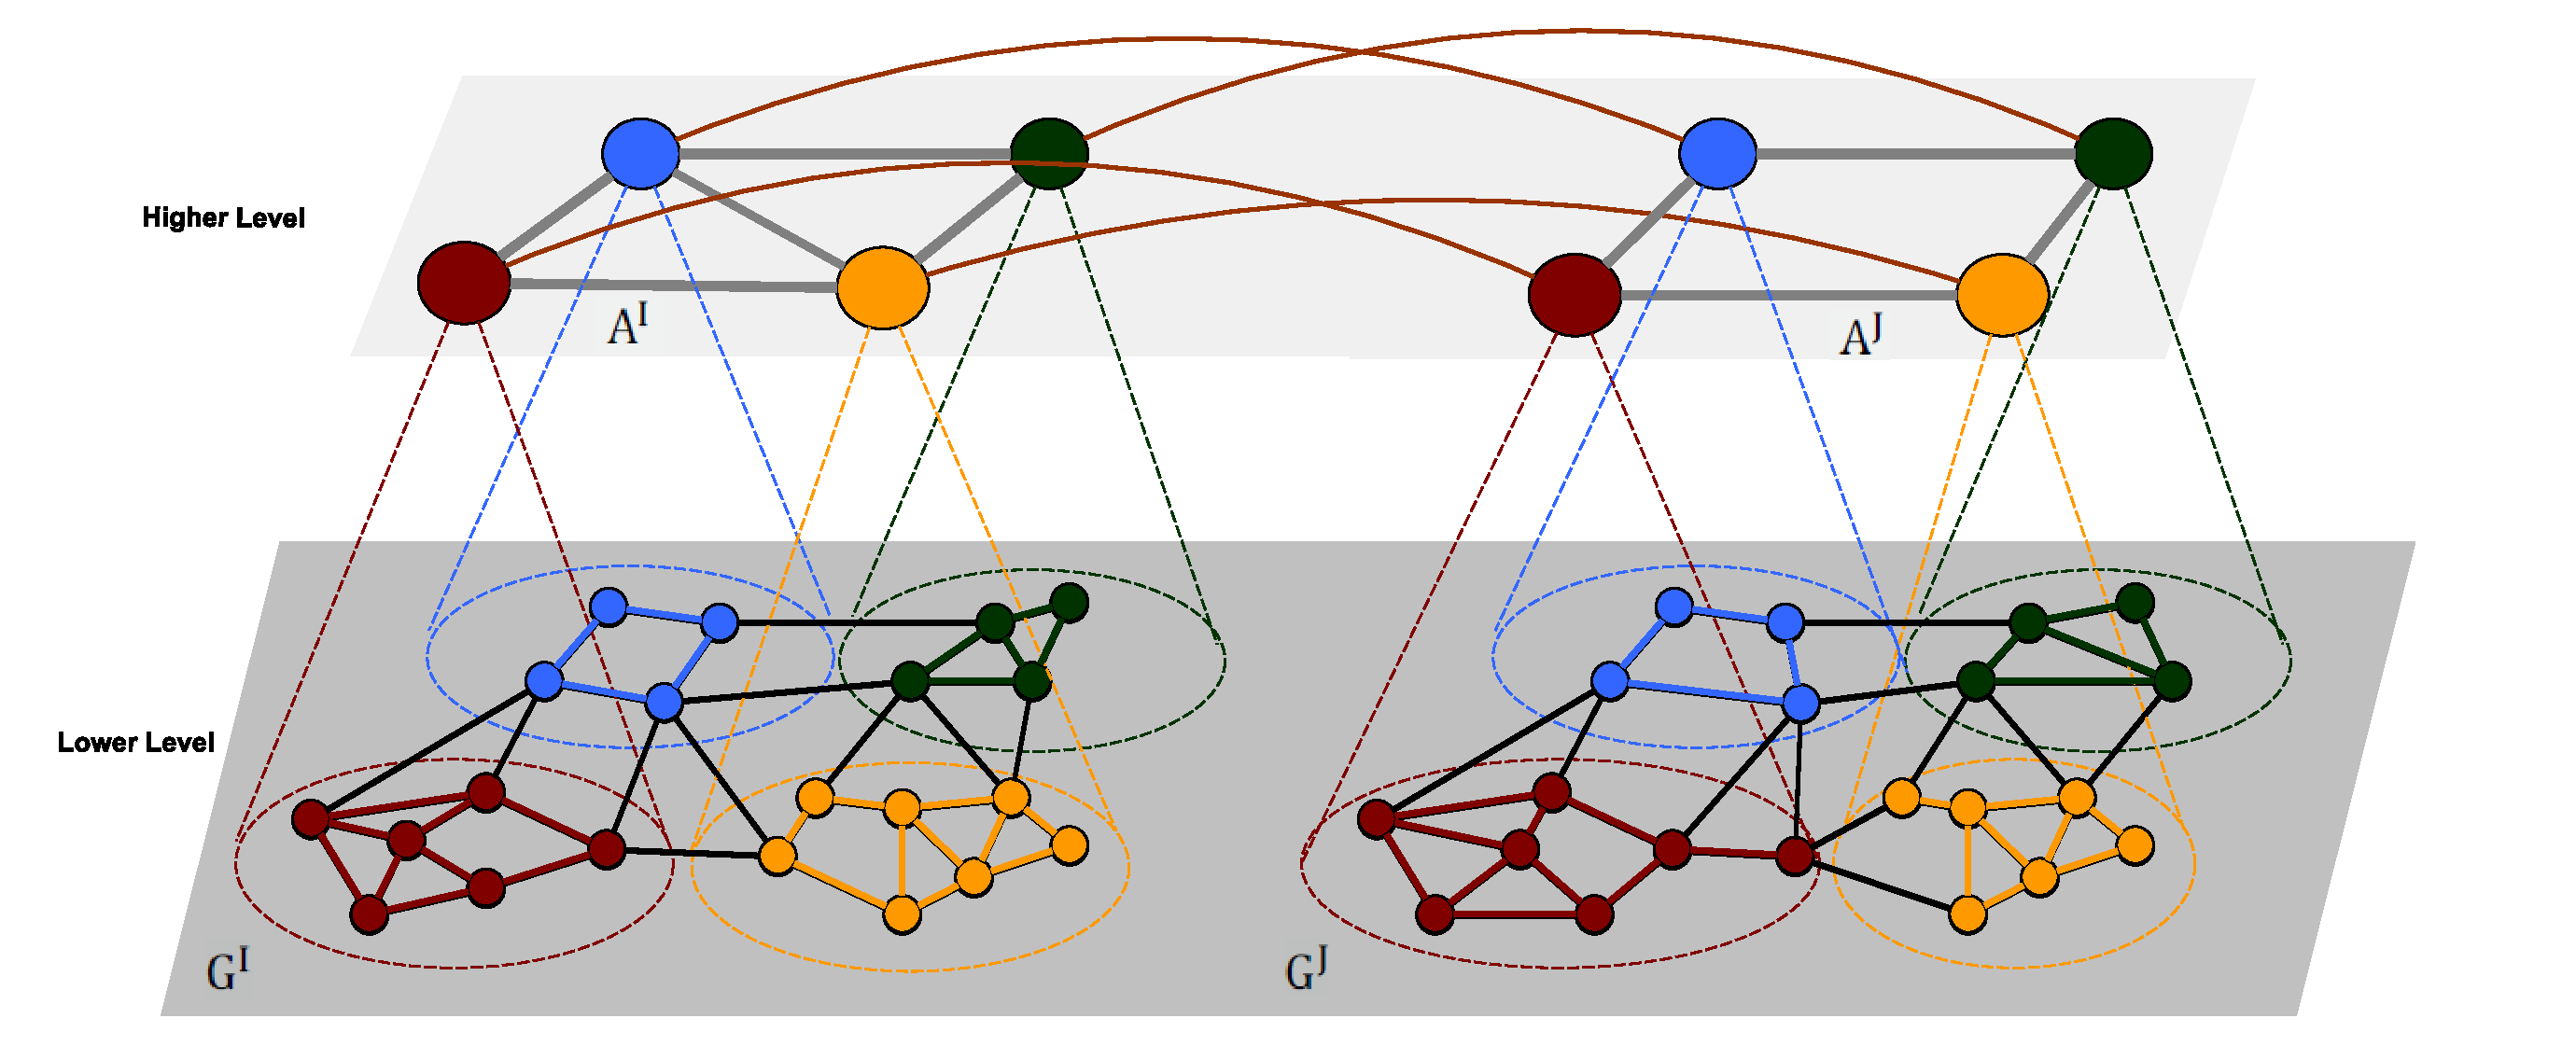
\includegraphics[scale=0.35]{chapter2/fig/twolevels3.pdf}
	\caption{Two level framework for graph matching} \label{fig:2levels}
\end{figure}

We return now back to the case of two graphs $G^I=(V^I,E^I,D^I)$ and $G^J=(V^J,E^J,D^J)$, which we want to match. 
For each of them we build an anchor graph $A^I=(V^{Ia},E^{Ia},U^{Ia})$ and $A^J=(V^{Ja},E^{Ja},U^{Ja})$ respectively.
Now instead of matching graphs $G^I$ and $G^J$ directly on the lower level, we may want to match first the corresponding anchor graphs. Matches between anchor nodes give us correspondences between underlying subgraphs. After that, we can perform graph matching for each pair of subgraphs independently. A union of local solutions from single subgraph matching problems gives us a solution of initial problem. 

Why can this approach be better than direct one? As we seen from the previous section the time and space complexity of the considering graph matching problem depends highly on the size of initial graphs. Constructed anchor graphs are however several time smaller than initial graphs, which means, the matching algorithm on the anchor level can be performed much faster and without high memory demand than on the lower level. The same holds for matching between the subgraphs.
%If $C(n)$ is complexity of a graph matching algorithm with $n$ possible correspondences.
Obviously, the accuracy of such two level matching approach depends heavily on the partition of the initial graphs into subgraphs and on the quality of a graph matching algorithm on both higher and lower levels. \ToDo{From this two critical moments we concentrate ourself on the first one}We concentrate ourself on the first of this two ctitical moments and use some existing algorithm for graph matching. To make the described two level approach more robust against graph partitioning we suggest to use an obtained matching between two graphs to correct their partitions. The \ToDo{all}whole procedure (matching on the higher level, matching on the lower level and partition updating) is then repeated iteratively till convergence of the objective function~\eqref{eq:gQAP1_2}. The algorithm is summarized below in Alg.\ref{alg:2levelGM}.

\begin{algorithm}[h]
	\KwIn{ initial graphs $G^I$, $G^J$\\
		   \hspace{45pt}maximal number of iterations $N$\\
		   \hspace{45pt}convergence parameters $R$ and $\epsilon$}
	\KwOut{set $m$ of correspondences between the nodes $V(G^I)$ and $V(G^J)$}
	construct anchor graph $A^I$ of the graph $G^I$ \label{alg:2levelGM_clustering1}\\
	construct anchor graph $A^J$ of the graph $G^J$ \label{alg:2levelGM_clustering2}\\
	i=0, $score_i$=0\\
	\While{$r<R$  \textbf{AND} $i\le N$}
	{ $i=i+1$ \\
	  \If{$i\ge 2$}
	  {update subgraphs $G[V^I_k],G[V^J_p],k=1\dots,m_1,\ p=1\dots,m_2$ \label{alg:2levelGM_update}}
	  match anchor graphs $A^I$,$A^J$ \label{alg:2levelGM_GM1} \\
	  $m_i=\emptyset$\\
	  \ForEach{pair of matched anchors $(a_k,a_p),a_k\in V(A^I), a_p\in V(A^J)$}
	  {match subgraphs $G[V^I_k]$,$G[V^J_p]$ \label{alg:2levelGM_GM2}\\
	   $m_i=m_i\cup\{m^k_i\}$\hspace{55pt}\tcc{$m^k_i$ set of local correspondences}
	  }
	  $score_i=x^TSx$ \hspace{5pt}\tcc{$x$ the indicator vector of the subset $m_i\subseteq M$}
	  \If{$|score_i-score_{i-1}|<\epsilon$}
	  {$r=r+1$}
	  \Else{$r=0$}
	}
	\Return $m_i$
	\caption{twoLevelGM($G^I$, $G^J$, $N$, $R$, $\epsilon$)} \label{alg:2levelGM}
\end{algorithm}

In the following we describe in details the single steps of our approach: %initial graph construction,
graph partitioning~(lines~\ref{alg:2levelGM_clustering1},\ref{alg:2levelGM_clustering2}), graph matching algorithm on both levels~(lines~\ref{alg:2levelGM_GM1},\ref{alg:2levelGM_GM2}), as well as update rule for current graph partitions~(line~\ref{alg:2levelGM_update}).
%\FloatBarrier
% ---------------------------------------        HLG Construction
\subsection{Anchor Graph Construction}
A problem of anchor graph construction for initially given graph $G^I=(V^I,E^I,D^I)$ turns straight forward into problem of partitioning the graph $G^I$. During our work on this thesis we tried out different strategies for clustering nodes of a given graph. Here we present those, which were more suitable for our matching framework, however generally an arbitrary algorithm for graph partitioning can be used.

Here and further we assume that the nodes of the given fine graph $G^I$ are located on a plane. That means, for each node we have additionally to its attribute an associated pair of coordinates and therefor can define the length of an edge as a $L^2-$distance between its endpoints. \ToDo{The reason for this assumption is given by practical applications such as image or object recognition.}
\subsubsection{Using grid}	
The first algorithm we describe is the most simple one. It uses a grid with fixed number of rows $r$, columns $c$ and a cell width $w$. The grid is placed over the graph $G^I$. Nodes, that are captured by a same grid cell belong to one cluster. Obviously, the number of clusters is equal to $r\times c$. We place anchor nodes in the middle of the grid cells. Two anchors are connected by an edge, if the cells they belong to have a common edge.
\subsubsection{Algorithms based on node merge}
The next considered approach creates an anchor graph $A^I$ with a predefined number $m_1$ of anchors. For that we adopted a coarsening phase from multi-level graph partition algorithms \cite{Chevalier09_GP, Safro2012_GC, Karypis95_GP, Hendrickson1995}.
Such algorithms have generally three phases: 
\begin{enumerate}
	\item graph coarsening phase, where one creates a hierarchy of graphs by successive merging of nodes in graph on previous stage starting with initial graph;
	\item graph partition phase, where the partition problem is solved exact on the coarsest level;
	\item refinement phase, where solution of the coarsest level is interpolated through all levels of the hierarchy until the initial graph.
\end{enumerate}
There are several types of graph coarsening algorithms. In our work we used so-called strict aggregation scheme (SAG)~\cite{Chevalier09_GP}, which groups nodes of $G^I$ in disjoint subsets based on the strength of the edges between them. We implemented two SAG based algorithms: Heavy Edge Matching (HEM) and Light Edge Matching (LEM)~\cite{Chevalier09_GP}. Both algorithms visit nodes of the graph $G^I$ in random order and construct an independent set of edges $E^\prime$ of the graph. The edge selection is based on the edge weights. The HEM picks and adds into $E^\prime$ the strongest edge adjacent to a current node $v$, that does not belong to the set of end nodes of edges in $E^\prime$.~(see Alg.~\ref{alg:HEM}). As opposed to this, the LEM selects the weakest edge adjacent to a current node. The edges in $E^\prime$ will be contracted, i.e. their endpoints will be replaced with a new node, that lies in the middle of a contracted edge and is connected to all neighbors of its endpoints.

%{\LinesNumberedHidden
%\LinesNumberedHidden
%\LinesNotNumbered
\begin{algorithm}[h]
	i = 0, $E^\prime=\emptyset$ \\
	\While{$|V(G^I)|>m_1$  \textbf{AND} $i\le N$}
	{ select a random node $v\in V(G^I)\setminus V(M)$ \\
	  \If{$\exists v^\prime=\argmax_{u\in V(G^I)\setminus V(M)} w(v,u)$}
	  {$E^\prime=E^\prime\cup{e_{vv^\prime}}$}
	  \Else{$i=i+1$}
	}
	\Return $G^I$
	\caption{HEM($G^I$, $m_1$, $N$)} \label{alg:HEM}
\end{algorithm}

In out case, graph $G^I$ is not initially weighted. To use the described coarsening methods we need to define a strength of graph edges. In case of LEM-Algotihm we set the length of an edge as its strength: $w_{vv^\prime}=\|v-v^\prime\|_{2}$. If we use HEM-Algorithm the strength of an edge is equal to $w_{ii^\prime} = exp(-\frac{\|v-v^\prime\|_{2}}{\sigma^2_{s}})$ with a constant $\sigma^2_{s}$.

It is clear, that one iteration of HEM or LEM reduces the number of nodes in $G$ at most by $\lfloor\frac{n}{2} \rfloor$ nodes. To get an coarse graph with $m_1$ nodes the coarsening algorithm should be repeated several times.

\subsection{Anchor graph matching}
In the previous section we have described how to construct anchor graphs $A^I=(V^{Ia},E^{Ia}, U^{Ia})$ and $A^J=(V^{Ja},E^{Ja},U^{Ja})$ of given graphs $G^I = (V^I, E^I, D^I)$ and $G^J=(V^J, E^J, D^J)$ respectively. Now, we focus our attention on the problem of matching two anchor graphs. For that, according to our problem formulation~\eqref{eq:gQAP1_2}-\eqref{eq:gQAP4_2}, we need to define a similarity matrix $S^A\in\mathbb{R}^{m_1m_2\times m_1m_2}$ between the graphs $A^I$ and $A^J$, where $m_1=|V^{Ia}|$ and $m_2=|V^{Ja}|$. This matrix contains two types of similarities: edge similarities (non-diagonal elements) and nodes similarities (diagonal elements).

Let us consider a pair of anchors  $a_k$, $a_k^\prime\in V^{Ia}$. We define the length of the edge $e_{kk^{\prime}}$ between those anchors as a median of distances between nodes in the corresponding subgraphs $G[V^I_k]$ and $G[V^I_{k^\prime}]$. With other words:
\begin{equation} L_{kk^\prime} = \median_{\substack{v_i\in G[V^I_k]\\ v_{i^\prime}\in G[V^I_{k^\prime}]} }\|v_i-v_{i^\prime}\|_{2}. \end{equation}
%where $\|v_i-v_{i^\prime}\|_{2}$ is the euclidean distance between the nodes $v_i\in G[V^I_k]$ and $v_{i^\prime}\in G[V^I_{k^\prime}]$.
Using this definition we calculate the similarity $s^A_E(e_{kk^\prime}, e_{pp^\prime})$ between edges $e_{kk^\prime}\in E^{Ia}$ and $e_{pp^\prime}\in E^{Ja}$ based on their length as it was done in the Eq.~\eqref{eq:edge_sim1}:
\begin{equation*}
s^A_E(e_{kk^\prime}, e_{pp^\prime}) = exp(-\frac{(L_{kk^\prime} - L_{pp^\prime})^2}{\sigma^2_{s}}).
\label{eq:s_e_A}
\end{equation*}

As we already discussed in the previous chapter, a natural way to define node similarities is to compare their attributes. However, our anchor graphs $A^{Ia}$, $A^{Ja}$ do not have direct attributes in contrast to the initial graphs $G^I$, $G^J$. Further we describe two ideas, how to go around this problem. %which we suggest to calculate anchor similarities.

The first idea would be to assign some attributes to the anchors and proceed further in the same way, as for initial graphs. Definition of those attributes in the same way, as for nodes of original graphs, meaning taking into account only the anchor graphs and not considering underlying initial graphs, will probably not give us good results. The reason for this is, that two anchors of different subgraphs can get similar attributes and therefor are likely to be selected by a matching algorithm. If it happens then the matching of the underlying subgraphs will have very low quality. This will have in turn an impact on the quality of the total matching of initial graphs. Consequently anchor attributes should incorporate the information about underlying subgraphs of original graphs.
Consider an anchor $a_k\in V^{Ia}$ and its underlying subgraph $G[V^I_k]=(V^I_k,E^I_k,D^I_k)$. We suggest two classes of attributes of the anchor $a_k$. 
\begin{itemize}
\item The first one uses a node attributes $D^I_k$ of the underlying subgraph $G[V^I_k]$. For this purpose we adopted \emph{bag of features model}~\cite{BoF_Leung2001}. We build once a common dictionary of all provided attributes in the both fine graphs by performing \emph{k-means clustering} of $D^I\cup D^J$ into $C$ clusters. Center of the clusters represent "codewords". Each attribute of a node in $V^I_k$ is afterwards mapped onto the closest codeword. In this way, the anchor attribute $d_1(a_k)\in\mathbb{R}^C$ is defined as normalized histogram of "codewords" in corresponding subgraphs.

\item The second class of attributes should capture the geometrical structure of underlying subgraph. We define $d_2(a_k)\in\mathbb{R}^{|V^I_k|\times b}$ as a set of $|V^I_k|$ histograms $\{d_2(a_k,v)\}$ with $b$ bins. Each histogram $d_2(a_k,v)$ represents a distribution of the length of the subgraph edges inside a small circle region around a node $v\in V^I_k$. 
\end{itemize}
The similarity value between two anchors can now be determined based on the first or second type of anchor attributes. To calculate a distance between histograms we use $\chi^2$ statistic test \cite{Weken2004_ChiSqTest}:
\begin{equation}
s^A_1(a_k, a_p) = \sum_{b_i\in B}\frac{(d_1(a_k,b_i)-d_1(a_p,b_i))^2}{(d_1(a_k,b_i)+d_1(a_p,b_i)},
\end{equation}
\begin{equation}
s^A_2(a_k, a_p) = \frac{1}{|V^I_k|}\frac{1}{|V^J_p|}\sum_{v\in V^I_k}\sum_{u\in V^J_p} \big(\sum_{b_i\in B}\frac{(d_2(a_k,v,b_i)-d_2(a_p,u,b_i))^2}{(d_2(a_k,v,b_i)+d_2(a_p,u,b_i))}\big),
\end{equation}
where $a_k\in A^I, a_p\in A^J$ and notation $d_1(a_k,b_i)$ and $d_2(a_k,v,b_i)$ denote a value in the $b_i$-th bin of the corresponding histogram. 
Both defined similarities can be used separately or set together as a linear combination into one similarity function.

The second idea to determine similarity $s^A(a_k, a_p)$ between two anchors could be to perform graph matching of the underlying subgraphs $G[V^I_k]$, $G[V^J_p]$ and take its score as a similarity measure. This idea has a great drawback of high computational complexity, because we need to perform in total $m_1m_2$ local matches. However, in this case the objective function of the matching problem on the lower level and the one on the anchor level are closer related. For example, in case when we do not consider edge similarities between anchors and work only with anchor similarities, the objective score on the higher level represent the lower bound of the objective function on the lower level.  %Among other, the both should have the same trend during the optimization process.
~\ToDo{Indeeded, this is true, because the objective function on the lower level in this case sonsist of two parts: the objective function on the higher level and additional summands, which sorrespond to the similarities of edges between clusters.}
% --------------------------        LLG Construction          ---------------------------------------
\subsection{Subgraph matching}
Given two corresponding subgraphs $G^I_{k}=(V^I_{k},E^I_{k},D^I_{k})$ and $G^J_{p}=(V^J_{p},E^J_{p},D^J_{p})$, we use cosine similarity of the node attributes to calculate node similarity between $V^I_{k}$ and $V^J_{p}$. For the pairwise edge similarity we used the same formula as in case of anchor matching (see Eq.\eqref{eq:edge_sim1}), i.e.\ 
\begin{equation*}
s_E(e_{ii^\prime}, e_{jj^\prime}) = exp(-\frac{(l_{ii^\prime} - l_{jj^\prime})^2}{\sigma^2_{s}})
\end{equation*}
where $l_{ii^\prime}$, $l_{jj^\prime} $ are the lengths of edges $e_{ii^\prime}\in E^I$ and $e_{jj^\prime}\in E^J$ respectively.
%In our work we concentrate ourself on the task of finding feature correspondences between two images. Features are collected using such popular feature detectors as SIFT~\cite{Lowe2004}, MSER~\cite{MSER}. Extracted features from two images define the sets of nodes $V^I$, $V^J$ of the graphs $G^I$, $G^J$ respectively. As node attributes $D^I$, $D^J$ we used SIFT descriptors~\cite{Lowe2004} with fixed orientation and scale. 
%The nodes of the graphs are connected vie edges with their $k$ nearest neighbors.

% -------------------------        Matching algorithm              -------------------------
\subsection{Graph matching algorithm}
%Generally, we are not restricted to use one specific algorithm for subgraph and anchor graph matching. In this thesis we used \emph{Reweighted Random Walks Method} (\textbf{RRWM})~\cite{Cho2010_RRWM}, as it shows high matching accuracy according to result in the original paper and is fast. It also showed good results in finding common subgraphs of two graphs in presence of outliers. At the end of this chapter we give for completeness an overview of this algorithm.
Generally, we are not restricted to use one specific algorithm for subgraph and anchor graph matching. In this thesis we used \emph{Reweighted Random Walks Method} (\textbf{RRWM})~\cite{Cho2010_RRWM}, as it shows high matching accuracy according to result in the original paper and is fast. It also shows good results in finding common subgraphs of two graphs in presence of outliers. At the appendix~\ref{appendixB} we give an overview of this algorithm.

% -------------------------        Level connection              -------------------------
\subsection{Graph partition update}
Assume, we solved the graph matching problem on the higher and on the lower levels. That means, we know pairs of correspondences between the anchor nodes $m^a = \{(a_k, a_p)|a_k\in V^{Ia}, a_p\in V^{Ja}\}$ and between the nodes of the original graphs $m = \{(v_i, v_j)|v_i\in V^{I}, v_j\in V^{J}\}$. The last set is the union of the local solutions of the graph matching problem between pairs of subgraphs, as it is defined by $m^a$.
The quality of the resulting solution $m$ depends, as we already mentioned, in our framework not only on the quality of the graph matching algorithm, but also on the graph partitioning algorithm.
The Fig.~\ref{fig:badpartition} shows an example of a partition of two equal graphs, so that the matching result of subgraphs will be very pure for all possible combinations of anchors matches.

\begin{figure}[h]
	\centering
	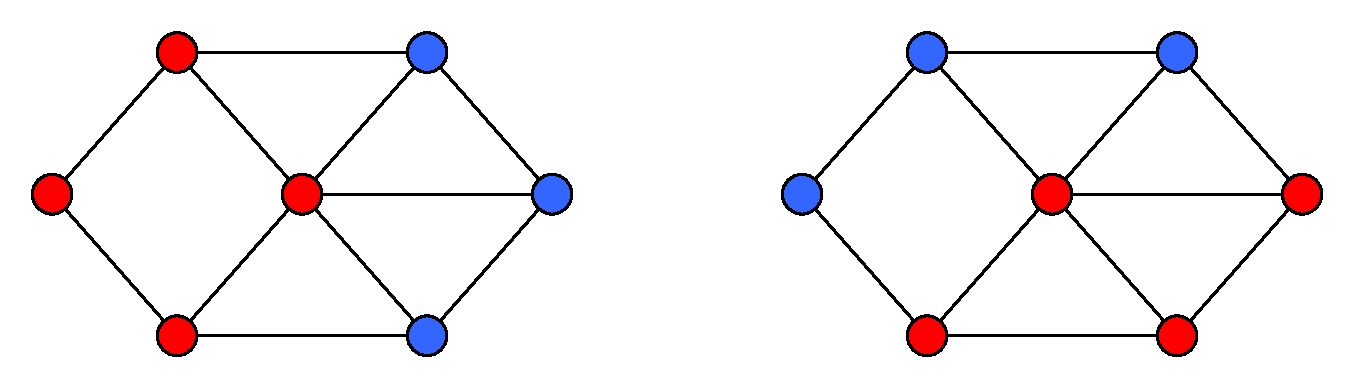
\includegraphics[scale=0.35]{chapter2/fig/badpartition.pdf}
	\caption[Example of bad partition of two equal graphs]{Example of bad partition of two equal graphs.} \label{fig:badpartition}
\end{figure}

To cope with such problems, we formulated our method as an iterative process. After each iteration the subgraphs of initial graphs have a chance to exchange nodes with their neighbors based on the obtained solution $m$ and improve matching quality of the next iteration. The proposed updating process consists of two major steps. In the first step we estimate an affine transformation between matched subgraphs based on the provided local correspondences. The next step is the actual update step, where updating process uses the estimated transformations.
We explain our approach on a pair of matched subgraphs $G[V^I_k]=(V^I_k, E^I_k, D^I_k)$ and $G[V^J_p]=(V^J_p, E^J_p, D^J_p)$  with obtained local correspondence set $m^{kp}=\{(v_i,v_j)|v_i\in V^I_k, v_j\in V^J_p\}$. 

In the first step we want to estimate two affine transformations $T_{kp}:V^I_k\rightarrow V^J_p$ and $T_{pk}:V^J_p\rightarrow V^I_k$ from the node set of one subgraph into another and vice versa. For that we use the  the state-of-the-art Coherent Point Drift~(CPD) algorithm by Myronenko and Song~\cite{Myronenko2009_CPD}. This is an probabilistic algorithm for points set registration problem, which finds a correspondences between two set of points and a transformation that describes the mapping between sets. We choose it, because it shows a remarkable robustness against outliers and often outperforms the other popular algorithm TPS-RPM by Chui and Rangarajan~\cite{Chui2003}, that we mentioned in the chapter~\ref{chapter:GM}. After obtaining the affine transformations $T_{kp}$ and $T_{pk}$ we measure a transformation error of each matched node $v_i\in V^I_k (v_j\in V^J_k)$ as a distance between its projection into other subgraph $T_{kp}(v_i) (T_{pk}(v_j))$ and its matched pair $m(v_i) = v_j\in V^J_p\ (m(v_j) = v_i\in V^I_k)$:
\begin{align}\begin{split} \label{eq:err_v}
err(v_i) &= \|T_{kp}(v_i) - m(v_i)\|_{2}\\
err(v_j) &= \|T_{pk}(v_j) - m(v_j)\|_{2}
\end{split}\end{align}
Based on the errors of single nodes we assign an error to the estimated transformations as a measure of their quality:
\begin{equation}\begin{split} \label{eq:err_T}
err(T_{kp}) & = \median_{v_i\in V^I_k}err(v_i) \\
err(T_{pk}) & = \median_{v_j\in V^J_p}err(v_j)
\end{split}\end{equation}
From both transformations we select the one with smallest error and replace the second with the inverse transformation of the selected one. For simplicity we preserve the notation $T_{kp}$ and $T_{pk}$ for the transformations related to the subgraph match $(a_k, a_p)$. In this way we associate with each subgraph pair with more than $3$ node correspondences \footnote{we need at least $3$ pair of correspondences to be able to estimate an affine transformation} to affine transformations between their nodes.

In the next step, we apply estimated transformations to each subgraph of both graphs to project them into the node space of the opposite graph (see Fig.~\ref{fig:update}). For the subgraph $G[V^J_p]$ that means, that the transformation $T_{pk}$ associated with the anchor pair $(a_k,a_p)$ is now casted as a mapping $T_{pk}:V^J_p\rightarrow V^I$. For the projected points $T_{pk}(v_j),v_j\in V^J_p,$ we find their nearest neighbors $\bar{v}_i=NN(T_{pk}(v_j))$ in $V^I$. In Fig.~\ref{fig:update} the projected points $T_{pk}(v_j),v_j\in V^J_p,$ are marked with bright red color. We define a new matrix $\bar{U}^{Ia}\in\mathbb{R}^{|V^I|\times m_1}$ and assign to its element $\bar{U}^{Ia}_{\bar{v}_i,a_k}=\|T_{pk}(v_j)-\bar{v}_i\|_2$ the distance between projection $T_{pk}(v_j)$ of $v_j\in V^J_p$ and its nearest neighbor $NN(T_{pk}(v_j))$ in $V^I$.

\begin{figure}[h]
	\centering
	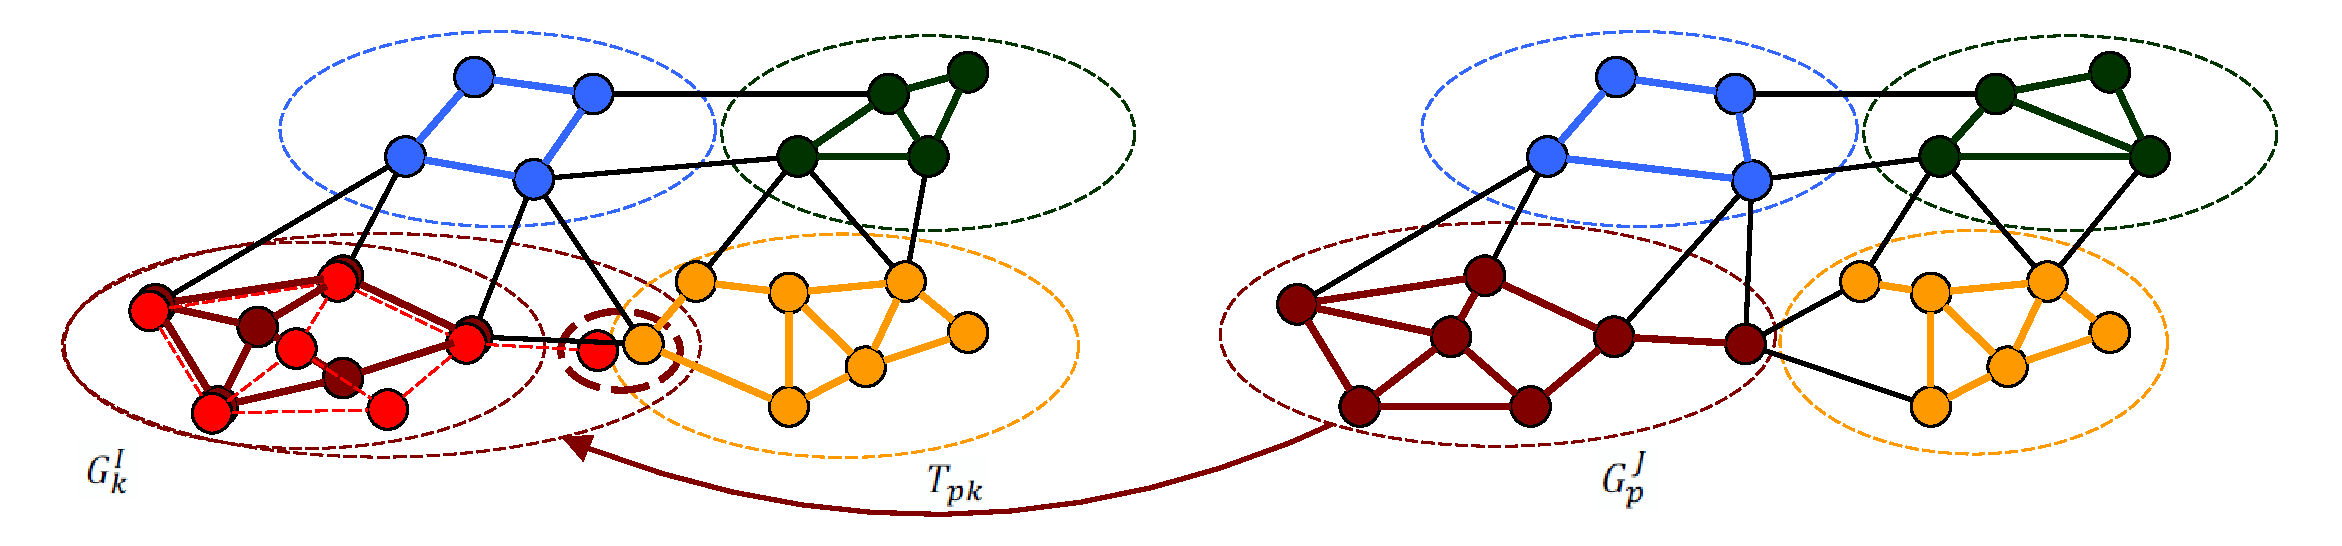
\includegraphics[scale=0.35]{chapter2/fig/update.pdf}
	\caption{Example of the graph partition update rule} \label{fig:update}
\end{figure}

After performing the same procedure for all transformations $T_{pk}$ we set all not-assigned elements of $\bar{U}^{Ia}$ to infinity. If there are some lines in $\bar{U}^{Ia}$ with all elements equal to infinity, meaning that corresponding nodes in $V^I$ were not selected as a nearest neighbor of the projections of the nodes in $V^J$,
then we replace those lines with the corresponding lines in the current matrix $U^{Ia}$ (see definition~\eqref{eq:matrixU}).

Our update rule for the partition of the graph $G^I$ defined by the matrix $U^{Ia}$ is:
\begin{equation}
U^{Ia}_{ik}=1 \iff a_k=\argmin_{l=1,\dots,m_1}^{}{\bar{U}^{Ia}_{v_i,a_l}}
\end{equation}
With the other words, the node $v_i\in V^I$ is assigned to the anchor $a_k$ if $\bar{U}_{v_i,a_k}$ is the smallest distance between $v_i$ and projections of the nodes in the subgraphs $G[V^J_p]$ matched to the subgraph $G[V^I_k]$. Note, that unassigned nodes in $V^I$ stay in the same cluster they were before. \ToDo{It also can happen, that one note on different iterations will be assigned to different clusters. This can be often the case on the border between two good estimated clusters. To prevent unnecessary jumps, we introduce a local memory of each node, where it saves information about clusters it belonged to and associated value of the matrix $\bar{U}^{Ia}$. We assign a node to a new cluster only when a new assignment is better than the previous ones.}

The partition of the second graph is updated in the same way, as it is described above for the graph $G^I$. The approach is summarized in Algorithm~\ref{alg:update_subgraphs4.3.2}.

\begin{algorithm}[h]
	\KwIn{  $m^a = \{(a_k, a_p)|a_k\in V^{Ia}, a_p\in V^{Ja}\}$\\
		\hspace{45pt}$m = \{(v_i, v_j)|v_i\in V^{I}, v_j\in V^{J}\}$}
	\KwOut{updated $U^{Ia}$, $U^{Ja}$}
	\tcc{Step $1$: assign affine transformations to each pair $(a_k, a_p)$ } 
	\ForEach{matched subgraph pair $(a_k, a_p)$}
	{
		calculate $T_{kp}:V^I_k\rightarrow V^J_p$ and $T_{pk}:V^J_p\rightarrow V^I_k$ using CPD algorithm
	}
	\tcc{Step $2$: calculate new matrices $\bar{U}^{Ia}\in\mathbb{R}^{|V^I|\times m_1}$, $\bar{U}^{Ja}\in\mathbb{R}^{|V^J|\times m_2}$ }
	\ForEach{matched subgraph pair $(a_k, a_p)$}
	{
		$\forall v_j\in V^J_p:\quad$ $\bar{U}^{Ia}_{\bar{v}_i,a_k}=\|T_{pk}(v_j)-\bar{v}_i\|_2$, where $\bar{v}_i=NN(T_{pk}(v_j))\in V^I$\\
		$\forall v_i\in V^I_k:\quad$ $\bar{U}^{Ja}_{\bar{v}_j,a_p}=\|T_{kp}(v_i)-\bar{v}_j\|_2$, where $\bar{v}_j=NN(T_{kp}(v_i))\in V^J$
	}
	\tcc{Step $3$: update partitions}
	$U^{Ia}_{ik}=1 \iff a_k=\argmin_{l=1,\dots,m_1}^{}{\bar{U}^{Ia}_{v_i,a_l}}$\\
	$U^{Ja}_{jp}=1 \iff a_p=\argmin_{q=1,\dots,m_2}^{}{\bar{U}^{Ja}_{v_j,a_q}}$\\
	\Return $U^{Ia}$, $U^{Ja}$
	
	\caption{UpdateSubgraphs}    \label{alg:update_subgraphs4.3.2}
\end{algorithm}

The usage of the proposed graph partition strategy is illustrated in Fig.~\ref{fig:update}. After performing the update procedure, the most left yellow node is likely to be included in the red partition, where in the fact it should belong to.
\FloatBarrier
% ---------------------------------------        Complexity
\subsection{Complexity}
We would like to investigate the \ToDo{asymptotic computational} complexity of our two level graph matching approach. For simplicity, we assume, that the complexity of a selected graph matching algorithm is $\mathcal{O}(f_{GM}(n_1,n_2))$, where $n_1$ and $n_2$ are the size of graphs we want to match.

The preprocessing step of our approach consists of two stages: initial graph partitioning and creation of the codebook of the node attributes. Note that the presence of the second stage depends on the selected strategy of the anchor graph matching. The complexity of the graph partitioning is in the worst case equal to $\mathcal{O}(n_2^2)$\footnote{We assumed $n_1\le n_2$}. Indeed, for one graph with $n$ nodes and $m$ anchors it is equal to $\mathcal{O}(nm)$ (using grid approach) or $\mathcal{O}((n-m)\Delta(G))$\footnote{We denote with $\Delta(G)$ the maximal degree of nodes in $V$, where degree of a node is equal to the number of its incident edges~\cite{Diestel2000}.} (HEM or LEM algorithm). The complexity of the codebook creation is determined by the complexity of clustering algorithm, which in case of Lloyd's k-means algorithm~\cite{kmeans_LLoyd} comes to $\mathcal{O}((n_1+n_2)rC)$ per iteration, where $r$ is dimension of the node attribute vectors and $C$ number of clusters. After joining those two results we obtain that the complexity of the preprocessing step is
\begin{equation}\label{eq:complexity1}
\mathcal{O}(n_2^2+(n_1+n_2)rCi),
\end{equation}where $i$ is the maximum number of iterations of the k-means clustering.

The main loop of our two level graph matching approach consists of three steps. The first one is the anchor graph matching, whose complexity is $\mathcal{O}(f_{GM}(m_1,m_2))$ plus complexity for initialization of the similarity matrix. In case, when we assign attributes to the anchors to calculate node similarity between two graphs, the complexity of the initialization can be approximated by $\mathcal{O}(m_1^2m_2^2)$. The complexity of the subgraph matching step afterwards results in $\sum_{(a_k,a_p)\in m^a}\mathcal{O}(f_{GM}(|V^I_k|,|V^J_p|))$. The complexity of two first steps in this case is equal to
\begin{equation}\label{eq:complexity2}
\mathcal{O}(m_1^2m_2^2)+\mathcal{O}(f_{GM}(m_1,m_2))+\sum_{(a_k,a_p)\in m^a}\mathcal{O}(f_{GM}(|V^I_k|,|V^J_p|)).
\end{equation}

In the case, when we use graph matching to determine the similarity between anchors, the complexity of both anchor and subgraph matching is equal to 
\begin{equation}
\sum_{(a_k,a_p)\in M^a}\mathcal{O}(f_{GM}(|V^I_k|,|V^J_p|)),\quad M^a=\{(a_k,a_p)|a_k\in V^{Ia},a_p\in V^{Ja}\},
\end{equation}because subgraph matching is already included in the anchor matching step.

At the end we only need to determine the complexity of our update rule. The CPD algorithm has linear complexity, which means we can estimate transformations between all matched subgraph with demand $\sum_{(a_k,a_p)\in M^a}\mathcal{O}(\max(|V^I_k|,|V^J_p|))$. The actual update step afterwards has the complexity $\mathcal{O}(n_1m_1+n_2m_2)$.

If we know assume, that we can completely parallelize the computation of the sum in Eq.~\eqref{eq:complexity2}, that the total complexity of the one iteration of our two level graph matching approach is equal to
\begin{equation}\label{eq:complexity3}
\begin{split}
\mathcal{O}(m_1^2m_2^2)&+\mathcal{O}(f_{GM}(m_1,m_2))+\mathcal{O}(f_{GM}(\max_{k}|V^I_k|,\max_{p}|V^J_p|))\\
                       &+\mathcal{O}(f_{GM}(\max_{k}|V^I_k|,\max_{p}|V^J_p|))+\mathcal{O}(n_1m_1+n_2m_2)
\end{split}
\end{equation}
or to
\begin{equation}\label{eq:complexity4}
\begin{split}
\mathcal{O}(m_1^2m_2^2)&+\mathcal{O}(f_{GM}(m_1,m_2))+\mathbf{m_2}\mathcal{O}(f_{GM}(\max_{k}|V^I_k|,\max_{p}|V^J_p|))\\
&+\mathcal{O}(f_{GM}(\max_{k}|V^I_k|,\max_{p}|V^J_p|))+\mathcal{O}(n_1m_1+n_2m_2)
\end{split}
\end{equation}
depending on the selected strategy for computing similarity between anchor graphs. Let us notice that the constant $m_2$ in the Eq.~\eqref{eq:complexity4} increases the complexity of the whole algorithm, when we use subgraph matching to calculate similarity between anchors.

However, because of the complexity of the graph matching is the most expensive (in case of RRWM $\mathcal{O}(f_{GM}(n_1,n_2))=\mathcal{O}(n_1^2n_2^2)$), it will fully beat the complexity of other steps and we can approximate both Eqs.~\eqref{eq:complexity3} and~\eqref{eq:complexity4} with
\begin{equation}\label{eq:complexity3.1}
\mathcal{O}(f_{GM}(m_1,m_2))+\mathcal{O}(f_{GM}(\max_{k}|V^I_k|,\max_{p}|V^J_p|))
\end{equation} 
and 
\begin{equation}\label{eq:complexity4.1}
\mathcal{O}(f_{GM}(m_1,m_2))+\mathbf{m_2}\mathcal{O}(f_{GM}(\max_{k}|V^I_k|,\max_{p}|V^J_p|))
\end{equation}
respectively.

It is obvious, that the resulting complexity of our graph matching framework depends highly on the number of made iterations and on the size of anchor graphs and subgraphs.


% -------------------------  Discussion ----------------------------------------------------------------------
\section{Discussion}
We have proposed a novel framework for solving a graph matching problem formulated as an quadratic assignment problem. Our framework is based on known matching algorithms, but helps to cope with some limitations of their application, such as big space demand and high computational time.
%Our framework does not represent a new matching algorithm, but helps an existing one to cope with some limitations of it application, such as big space demand and high computational time.
Its core idea is to decompose an initial graph matching problem into a set of subproblems. For that we partition graphs into subgraphs, perform matching to determine pairs of subgraphs and than perform matching again independently for each pair of subgraphs. An obtained at the end solution is used to update graph partition. The whole procedure is repeated iteratively till convergence. The complexity of the proposed method depends highly on the complexity of the used graph matching algorithm, which in its turn depends on the size of the anchor graph and graph subgraphs. In the next chapter we evaluate the proposed framework on the synthetic and real data examples.
\ToDo{In the next chapter we apply the proposed framework to the synthetic and real data examples.}
  \chapter{Evaluation results} \label{chapter:results}

In this chapter we explore the quality of the proposed two level graph matching framework (we call it further 2LevelGM) on synthetic and real examples. The quality is measured by the matching score and accuracy of an obtained solution together with the running time in seconds needed to find it. Note, that under accuracy we understand actually recall of the graph matching algorithms (i.e. number of correct detected matches divided by the number of all correct matches), as it is done in~\cite{Cho2010_RRWM,Cho2012_ProgressiveGM,Cho2014_Haystack,Duchenne2011,Rangarajan1996_GAGM,Leordeanu2005_SM,Leordeanu2009_IPFP}.
To rate the usefulness of 2LevelGM we provide a comparison study across different graph matching algorithms. All tests in this chapter have been executed on a computer with an Intel(R) Core(R) i5-3210M CPU 2.50GHz with $4$ cores unless otherwise specified. We implemented our framework in the software package MATLAB and used $2$ workers\footnote{For more details see~\url{http://mathworks.com/help/distcomp/parallel-pools.html}} to run 2LevelGM. The code was not optimized. The sources of additionally used libraries and algorithms for comparisons are referred directly in the text. %To make the comparison between the algorithms fair we used in all cases the same greedy assignment algorithm~\cite{Leordeanu2005_SM} for discretization of an obtained continuous solution. We also included the initialization and discretization steps into the runtime measurement.
To make the comparison fair we have measured the running time of all algorithms from the initialization step till an final discrete solution is found. We also have used the greedy assignment algorithm~\cite{Leordeanu2005_SM} to discretize continuous solutions, obtained by some algorithms.

\section{Synthetic data}
For the first set of tests we adopted a commonly used approach for evaluation of graph matching algorithms on two synthetic generated sets of points (see \cite{Cho2010_RRWM,Cho2014_Haystack,Leordeanu2009_IPFP}). 
For this purpose one generates first a set $V^I\subset\mathbb{R}^2$ of $n_1$ standard normally distributed points on a plane: $V^I=\{v_i=(x_i,y_i)|x_i\sim\mathcal{N}(0,1),y_i\sim\mathcal{N}(0,1),i=1,\dots,n_1\}$. In a second step $V^J$ is generated, which represents a distorted copy of the first set with $\bar{n}$ additional normally distributed points. The distortion is achieved by adding a normally distributed noise with zero mean and a variance $\sigma^2$ to the coordinates of the points in $V^I$. 
%The parameter $\sigma$ expresses the deformation in the second set $V^J$.
This means, that the set $V^J$ consists of $n_2=n_1+\bar{n}$ nodes, where $n_1$ points have a unique pair in $V^I$ and are called inliers, whereby the other $\bar{n}$ points are outliers. The task is to find correspondences between points in the two sets, which obviously can be formulated as a graph matching problem. For that we consider two fully connected graphs $G^I$ and $G^J$ with nodes defined by the sets $V^I$ and $V^J$ respectively. We assume, that the graphs do not have attributes and each node in the first graph can be theoretically matched to each node in the second graph.

For the evaluation of 2LevelGM we follow the setup of the synthetic point set tests from publications~\cite{Cho2014_Haystack} and \cite{FastPFP} and formulate four different kinds of tests. In the first test we set the number of outliers $\bar{n}$ to zero and vary only the deformation noise $\sigma^2$. In the second test, we do not have a deformation noise ($\sigma^2=0$) and compare the behavior of the different graph matching algorithms in case of an increasing number of outliers $\bar{n}$. In the third test, we perform the second test in presence of deformation in the second graph. For this we fix $\sigma^2= 0.03$ and increase iteratively the number of outliers $\bar{n}$. Finally, in the fourth test we consider again two graphs with the same size, but omit randomly $(1-\theta)$ percentage of edges in both graphs with increasing $\theta$. 
For performing the tests we used the supplemental MATLAB code provided by Minsu Cho et al. in their paper~\cite{Cho2014_Haystack}. For simplicity we combine the described tests together in a first group of tests. %and present results of its test below.We combine the described tests in one group and perform further a comparison of graph matching algorithms on two such groups, that differ in the size of considered graphs inside them. 

The first graphs we consider are relatively small: $100-150$ nodes. The main reason for using small graphs is to compare the 2LevelGM with the following well known methods: MPM~\cite{Cho2014_Haystack}, RRWM~\cite{Cho2010_RRWM}, SM~\cite{Leordeanu2005_SM} and IPFP~\cite{Leordeanu2009_IPFP}\footnote{We used the implementation of those algorithms provided in~\cite{code_MPM}.}. The selection of the graph size was determined by application examples of the corresponding algorithms provided in the mentioned publications. To our best knowledge, those algorithms have not been applied directly to graphs with more than $150$ nodes each without additional problem simplifications (for example reduction of the set of possible correspondences, which is difficult to achieve for non-attributed graphs). This restriction on the size of the graphs is determined mainly by the size of the dense affinity matrix $S$, which is used by all algorithms. The matrix $S$ is calculated in all cases using Eq.~\eqref{eq:edge_sim1_2} with $\sigma_s^2=0.15$, where the value of the parameter $\sigma_s^2$ is chosen according to the proposition made in~\cite{Cho2010_RRWM}. To calculate the affinity matrix on the anchor level we use $\sigma_s^2=10$. 

Since our initial graphs $G^I$ and $G^J$ are not attributed, we first consider the formulation of 2LevelGM with non-attributed anchors graphs. The similarities between anchors are calculated in this case based on the matching score of the underlying subgraphs (see chapter~\ref{anchorGraphMatching}). For the initialization of the initial subgraphs we use the grid method (see chapter~\ref{subgraphInit}) with $2\times 2$ cells. The average matching results of $10$ runs in the four defined tests are illustrated in Figs.~\ref{fig:synTest1_ver433}-\ref{fig:synTest4_ver433}. The vertical bars at each point show the standard deviation of the measured mean value (accuracy, objective score and running time) for the corresponding problem setting.
% -----------------------------  Version 4.3.3    -------------------------------
\begin{figure}
	\begin{subfigure}[b]{0.33\textwidth}
		\centering
		\includegraphics[scale=0.25]{"chapter3/fig/SyntheticTest/no_descr/Results_v4.3.3/Test2/accuracy_avg10t"} 
	\end{subfigure}
	\begin{subfigure}[b]{0.33\textwidth}
		\centering
		\includegraphics[scale=0.25]{"chapter3/fig/SyntheticTest/no_descr/Results_v4.3.3/Test2/score_avg10t"} 
	\end{subfigure} 
	\begin{subfigure}[b]{0.32\textwidth}
		\centering
		\includegraphics[scale=0.33]{"chapter3/fig/SyntheticTest/no_descr/Results_v4.3.3/Test2/time_summary_avg10t"} 
	\end{subfigure} 
	\caption[Performance of the 2LevelGM with non-attributed anchor graphs on synthetic data (test $1$)]{Performance of the 2LevelGM with non-attributed anchor graphs on synthetic data: test $1$ ($n_1=100$, $\bar{n}=0$, $\theta=100\%$)}
	\label{fig:synTest1_ver433}
\end{figure}
%\vspace{-20pt}
\begin{figure}
	\begin{subfigure}[b]{0.33\textwidth}
		\centering
		\includegraphics[scale=0.25]{"chapter3/fig/SyntheticTest/no_descr/Results_v4.3.3/Test3/accuracy_avg10t"} 
	\end{subfigure}%% 
	\begin{subfigure}[b]{0.33\textwidth}
		\centering
		\includegraphics[scale=0.25]{"chapter3/fig/SyntheticTest/no_descr/Results_v4.3.3/Test3/score_avg10t"} 
	\end{subfigure} 
	\begin{subfigure}[b]{0.33\textwidth}
		\centering
		\includegraphics[scale=0.33]{"chapter3/fig/SyntheticTest/no_descr/Results_v4.3.3/Test3/time_summary_avg10t"} 
	\end{subfigure} 	
	\caption[Performance of the 2LevelGM with non-attributed anchor graphs on synthetic data (test $2$)]{Performance of the 2LevelGM with non-attributed anchor graphs on synthetic data: test $2$ ($n_1=100$, $\bar{n}\in[0,50]$, $\sigma^2=0$, $\theta=100\%$)}
	\label{fig:synTest2_ver433}
\end{figure}
%\vspace{-20pt}
\begin{figure}
		\begin{subfigure}[b]{0.33\textwidth}
			\centering
			\includegraphics[scale=0.25]{"chapter3/fig/SyntheticTest/no_descr/Results_v4.3.3/Test1/accuracy_avg10t"} 
		\end{subfigure}%% 
		\begin{subfigure}[b]{0.33\textwidth}
			\centering
			\includegraphics[scale=0.25]{"chapter3/fig/SyntheticTest/no_descr/Results_v4.3.3/Test1/score_avg10t"} 
		\end{subfigure} 
		\begin{subfigure}[b]{0.33\textwidth}
			\centering
			\includegraphics[scale=0.33]{"chapter3/fig/SyntheticTest/no_descr/Results_v4.3.3/Test1/time_summary_avg10t"} 
		\end{subfigure} 	
	\caption[Performance of the 2LevelGM with non-attributed anchor graphs on synthetic data (test $3$)]{Performance of the 2LevelGM with non-attributed anchor graphs on synthetic data: test $3$ ($n_1=100$, $\bar{n}\in[0,50]$, $\sigma^2=0.03$, $\theta=100\%$)}
	\label{fig:synTest3_ver433}
\end{figure}
%\vspace{-20pt}
\begin{figure}
		\begin{subfigure}[b]{0.33\textwidth}
			\centering
			\includegraphics[scale=0.25]{"chapter3/fig/SyntheticTest/no_descr/Results_v4.3.3/Test4/accuracy_avg10t"} 
		\end{subfigure}%% 
		\begin{subfigure}[b]{0.33\textwidth}
			\centering
			\includegraphics[scale=0.25]{"chapter3/fig/SyntheticTest/no_descr/Results_v4.3.3/Test4/score_avg10t"} 
		\end{subfigure} 
		\begin{subfigure}[b]{0.33\textwidth}
			\centering
			\includegraphics[scale=0.33]{"chapter3/fig/SyntheticTest/no_descr/Results_v4.3.3/Test4/time_summary_avg10t"} 
		\end{subfigure} 	
	\caption[Performance of the 2LevelGM with non-attributed anchor graphs on synthetic data (test $4$)]{Performance of the 2LevelGM with non-attributed anchor graphs on synthetic data: test $4$ ($n_1=n_2=100$, $\sigma^2=0$)}
	\label{fig:synTest4_ver433}
\end{figure}
%\FloatBarrier
%-------------------------------------------------------------------------------

From this results one can see that the SM algorithm has the worst matching quality in all cases. 2LevelGM performs a little bit unstable, which is indicated by a relatively high standard deviation compared with other algorithms. For this reason the average performance (objective score and accuracy) of 2LevelGM is a little bit lower than the one of IPFP and RRWM, although in individual runs 2LevelGM is not worse. The running time of 2LevelGM is slower as of IPFP and RRWM. However this is expected, because without anchor attributes 2LevelGM performs graph matching using RRWM on each pair of subgraphs. Although those subgraphs are smaller than the initial graphs, the overall complexity of 2LevelGM is in this case higher as for the case RRWM is used standalone. This results in a longer runtime of 2LevelGM.
The slowest algorithm in this comparison is MPM. Nevertheless MPM achieved  best accuracy and objective score in three of four tests. However, it is outperformed by 2LevelGM in the first test (Fig.~\ref{fig:synTest1_ver433}) with significantly smaller time demand\footnote{The used implementations of 2LevelGM, SM and IPFP are purely MATLAB implementations, whereby some steps of MPM and RRWM were written using $C++$. This makes the comparison of the running time between algorithms difficult.}.

Below we present the results of testing on the first group of tests using 2LevelGM with attributed anchor graphs. For this purpose we use the attributes, that capture geometrical structure of the subgraphs (see chapter~\ref{anchorGraphMatching}). We set the size of used histograms to $35$ bins and the radius $R$ of the circle region around each node to $2$. The results of the comparison are presented in Figs.~\ref{fig:synTest1_descr_ver433}-\ref{fig:synTest4_descr_ver433}. One can directly see the improved performance time of the 2LevelGM algorithm in all tests. The proposed algorithm also shows a more stable performance in the second test. 
%, which practically solves subgraph the isomorphism problem.
On the other side, 2LevelGM seems to be more susceptible to graph deformations (see Figs.~\ref{fig:synTest1_descr_ver433}, \ref{fig:synTest4_descr_ver433}). The reason for this lies in the selected anchor attributes, that are not sufficiently robust against deformations in the length of edges.

% -----------------------------  Version 4.3.3    -------------------------------
\begin{figure}[h]
	\begin{subfigure}[b]{0.33\textwidth}
		\centering
		\includegraphics[scale=0.25]{"chapter3/fig/SyntheticTest/descr/Results_v4.3.3/Test2/accuracy_avg10t"} 
	\end{subfigure}
	\begin{subfigure}[b]{0.33\textwidth}
		\centering
		\includegraphics[scale=0.25]{"chapter3/fig/SyntheticTest/descr/Results_v4.3.3/Test2/score_avg10t"} 
	\end{subfigure} 
	\begin{subfigure}[b]{0.31\textwidth}
		\centering
		\includegraphics[scale=0.33]{"chapter3/fig/SyntheticTest/descr/Results_v4.3.3/Test2/time_summary_avg10t"} 
	\end{subfigure} 
	\caption[Performance of the 2LevelGM with attributed anchor graphs on synthetic data (test $1$)]{Performance of the 2LevelGM with attributed anchor graphs on synthetic data: test $1$ ($n_1=100$, $\bar{n}=0$, $\sigma^2=0$)}
	\label{fig:synTest1_descr_ver433}
\end{figure}
%\vspace{-25pt}
\begin{figure}[h]
	\begin{subfigure}[b]{0.33\textwidth}
		\centering
		\includegraphics[scale=0.25]{"chapter3/fig/SyntheticTest/descr/Results_v4.3.3/Test3/accuracy_avg10t"} 
	\end{subfigure}%% 
	\begin{subfigure}[b]{0.33\textwidth}
		\centering
		\includegraphics[scale=0.25]{"chapter3/fig/SyntheticTest/descr/Results_v4.3.3/Test3/score_avg10t"} 
	\end{subfigure} 
	\begin{subfigure}[b]{0.33\textwidth}
		\centering
		\includegraphics[scale=0.33]{"chapter3/fig/SyntheticTest/descr/Results_v4.3.3/Test3/time_summary_avg10t"} 
	\end{subfigure} 	
	\caption[Performance of the 2LevelGM with attributed anchor graphs on synthetic data (test $2$)]{Performance of the 2LevelGM with attributed anchor graphs on synthetic data: test $2$ ($n_1=100$, $\bar{n}\in[0,50]$, $\sigma^2=0$, $\theta=100\%$)}
	\label{fig:synTest2_descr_ver433}
\end{figure}
%\vspace{-25pt}
\begin{figure}[h]
		\begin{subfigure}[b]{0.33\textwidth}
			\centering
			\includegraphics[scale=0.25]{"chapter3/fig/SyntheticTest/descr/Results_v4.3.3/Test1/accuracy_avg10t"} 
		\end{subfigure}%% 
		\begin{subfigure}[b]{0.33\textwidth}
			\centering
			\includegraphics[scale=0.25]{"chapter3/fig/SyntheticTest/descr/Results_v4.3.3/Test1/score_avg10t"} 
		\end{subfigure} 
		\begin{subfigure}[b]{0.33\textwidth}
			\centering
			\includegraphics[scale=0.33]{"chapter3/fig/SyntheticTest/descr/Results_v4.3.3/Test1/time_summary_avg10t"} 
		\end{subfigure} 	
	\caption[Performance of the 2LevelGM with attributed anchor graphs on synthetic data (test $3$)]{Performance of the 2LevelGM with attributed anchor graphs on synthetic data: test $3$ ($n_1=100$, $\bar{n}\in[0,50]$, $\sigma^2=0.03$, $\theta=100\%$)}
	\label{fig:synTest3_descr_ver433}
\end{figure}
%\vspace{-25pt}
\begin{figure}[h]
		\begin{subfigure}[b]{0.33\textwidth}
			\centering
			\includegraphics[scale=0.25]{"chapter3/fig/SyntheticTest/descr/Results_v4.3.3/Test4/accuracy_avg10t"} 
		\end{subfigure}%% 
		\begin{subfigure}[b]{0.33\textwidth}
			\centering
			\includegraphics[scale=0.25]{"chapter3/fig/SyntheticTest/descr/Results_v4.3.3/Test4/score_avg10t"} 
		\end{subfigure} 
		\begin{subfigure}[b]{0.33\textwidth}
			\centering
			\includegraphics[scale=0.33]{"chapter3/fig/SyntheticTest/descr/Results_v4.3.3/Test4/time_summary_avg10t"} 
		\end{subfigure} 	
	\caption[Performance of the 2LevelGM with attributed anchor graphs on synthetic data (test $4$)]{Performance of the 2LevelGM with attributed anchor graphs on synthetic data: test $4$ ($n_1=n_2=100$, $\sigma^2=0.00$)}
	\label{fig:synTest4_descr_ver433}
\end{figure}
% --------------------------------------------------------------------------------

To test the performance of 2LevelGM on bigger graphs we created another group of three tests and compare the results of 2LevelGM with those of the  PATH~\cite{Zazlavskiy2008_PATH}\footnote{\url{http://cbio.ensmp.fr/graphm/}} and GLAG~\cite{Fiori2013_GLAG}\footnote{\url{http://www.fing.edu.uy/~mfiori/}. We replaced the default maximal number of iterations ($30000$) with $1000$ to reduce the computational time.} algorithms. In contrast to the graph matching problem formulation considered by 2LevelGM and previous algorithms the PATH and GLAG algorithms solve the minimization problem~\eqref{eq:QAP1}. However, they do not take into account node attributes, so the second term in~\eqref{eq:QAP1} disappears. PATH and GLAG do not work with the affinity matrix $S$ and therefore can be directly applied to bigger graphs without the necessity to reduce the set of possible candidate matches. This was the reason, why we have selected this algorithms to estimate matching results of our approach on bigger graphs. The results of the comparison in one run can be seen in Figs.~\ref{fig:synTest1_bigGraphs_ver433}-\ref{fig:synTest3_bigGraphs_ver433}\footnote{This group of tests was executed on a desktop PC with an 2.67GHz Intel(R) Xeon(R) CPU with $4$ cores. $4$ MATLAB workers were used}. We do not provide averaged results for this group of tests due to their high computational demand. The presented results were obtained by using $5\times 4$ grid to initialize 2LevelGM. The PATH and GLAG algorithms are initialized with the weighted adjacency matrices of the initial graph, whereby weights are defined by the length of the edges.
\FloatBarrier

\begin{figure}[h] 
		\begin{subfigure}[b]{0.33\textwidth}
			\centering
			\includegraphics[scale=0.25]{"chapter3/fig/SyntheticTest_BigGraphs/descr/Results_v4.3.3/Test1/accuracy_avg1t"} 
		\end{subfigure}
		\begin{subfigure}[b]{0.33\textwidth}
			\centering
			\includegraphics[scale=0.25]{"chapter3/fig/SyntheticTest_BigGraphs/descr/Results_v4.3.3/Test1/score_avg1t"} 
		\end{subfigure} 
		\begin{subfigure}[b]{0.32\textwidth}
			\centering
			\includegraphics[scale=0.33]{"chapter3/fig/SyntheticTest_BigGraphs/descr/Results_v4.3.3/Test1/time_summary_avg1t"} 
		\end{subfigure} 	
	\caption[Performance comparison of 2LevelGM, GLAG and PATH on bigger graphs: test $1$]{Performance comparison of 2LevelGM, GLAG and PATH on bigger graphs ($\bar{n}=0$, $\sigma^2=0$, $\theta=100\%$)}
	\label{fig:synTest1_bigGraphs_ver433}
\end{figure}
\begin{figure}[h] 
		\begin{subfigure}[b]{0.33\textwidth}
			\centering
			\includegraphics[scale=0.25]{"chapter3/fig/SyntheticTest_BigGraphs/descr/Results_v4.3.3/Test2/accuracy_avg1t"} 
		\end{subfigure}
		\begin{subfigure}[b]{0.33\textwidth}
			\centering
			\includegraphics[scale=0.25]{"chapter3/fig/SyntheticTest_BigGraphs/descr/Results_v4.3.3/Test2/score_avg1t"} 
		\end{subfigure} 
		\begin{subfigure}[b]{0.32\textwidth}
			\centering
			\includegraphics[scale=0.33]{"chapter3/fig/SyntheticTest_BigGraphs/descr/Results_v4.3.3/Test2/time_summary_avg1t"} 
		\end{subfigure} 	
	\caption[Performance comparison of 2LevelGM, GLAG and PATH on bigger graphs: test $2$]{Performance comparison of 2LevelGM, GLAG and PATH on bigger graphs ($\bar{n}=0$, $\sigma^2=0.03$, $\theta=100\%$)}
	\label{fig:synTest2_bigGraphs_ver433}
\end{figure}
\begin{figure}[h] 
		\begin{subfigure}[b]{0.33\textwidth}
			\centering
			\includegraphics[scale=0.25]{"chapter3/fig/SyntheticTest_BigGraphs/descr/Results_v4.3.3/Test3/accuracy_avg1t"} 
		\end{subfigure}
		\begin{subfigure}[b]{0.33\textwidth}
			\centering
			\includegraphics[scale=0.25]{"chapter3/fig/SyntheticTest_BigGraphs/descr/Results_v4.3.3/Test3/score_avg1t"} 
		\end{subfigure} 
		\begin{subfigure}[b]{0.32\textwidth}
			\centering
			\includegraphics[scale=0.33]{"chapter3/fig/SyntheticTest_BigGraphs/descr/Results_v4.3.3/Test3/time_summary_avg1t"} 
		\end{subfigure} 	
	\caption[Performance comparison of 2LevelGM, GLAG and PATH on bigger graphs: test $3$]{Performance comparison of 2LevelGM, GLAG and PATH on bigger graphs ($\bar{n}=0$, $\sigma^2=0$, $\theta=90\%$)}
	\label{fig:synTest3_bigGraphs_ver433}
\end{figure}

All performed tests for bigger graphs can be considered as instances of the graph isomorphism problem in exact (Fig.~\ref{fig:synTest1_bigGraphs_ver433}) and inexact (Figs.~\ref{fig:synTest2_bigGraphs_ver433},~\ref{fig:synTest3_bigGraphs_ver433}) forms. We investigate the matching score, accuracy and running time of the graph matching algorithms as functions of number of nodes in the initial graphs.
In all cases 2LevelGM outperforms both GLAG and PATH in objective score and especially in running time with one exception. This one is the running time of the last iteration in Fig.~\ref{fig:synTest2_bigGraphs_ver433}. We consider it as an individual case and suppose, that an imbalanced graph partitioning of initial graphs causes the jump in the running time. Overall 2LevelGM shows a high matching accuracy in all three tests. Additionally we believe it is possible to improve the framework by solving instability issues, which we saw in previous cases. 
\FloatBarrier
% --------------------------------------------------------------------
% --------------------------------------------------------------------
\section{Real data tests}
In the following sections we use the developed two level graph matching algorithm for finding correspondences between features on a pair of images. To formulate this problem as a graph matching problem we use the standard approach settled in computer vision literature~\cite{Cho2010_RRWM,Cho2012_ProgressiveGM,FastPFP,Hancock_EM_SVD,Hancock_GM_SpectralPart}. For that we extract SIFT features~\cite{Lowe2004} of two images around keypoints, that were located using some feature detector (we used  MSER~\cite{MSER}). Given the extracted features of two images we construct two attributed graphs $G^I=(V^I,E^I,D^I)$ and $G^J=(V^J,E^J,D^J)$ for each image respectively. The nodes of those graphs are placed at the locations of the detected keypoints with their features as node attributes. To connect nodes via edges one can use Delaunay triangulation~\cite{Hancock_EM_SVD,Hancock_GM_SpectralPart}, nearest neighbors relations between nodes~\cite{Sanrom2012} or consider complete graphs~\cite{Cho2012_ProgressiveGM,Cho2014_Haystack}.

\subsection{Image affine transformation}
The first image set we consider can be seen as a synthetic data set of real images. It consists of image pairs, where one image in each pair is the same in all cases and the second image represent a rotated/shifted copy of the first one with additional Gaussian noise added to its pixels (see Fig.~\ref{fig:ImageTrafo_initGraphs}\footnote{The presented image of a church is taken from the SUN\cite{SUN} dataset (category "church outdoor").}). On this simple examples we want to demonstrate the work of the update rule inside the 2LevelGM algorithm (see chapter~\ref{updateRule}).

\begin{figure}[h] 
		\begin{subfigure}[b]{0.3\textwidth}
			\centering
			\includegraphics[width=4cm]{"chapter3/fig/ImageTrafo/Img_pair1"} 
			\caption{}\label{fig:ImageTrafo_initGraphs_a}
		\end{subfigure}
		\begin{subfigure}[b]{0.3\textwidth}
			\centering
			\includegraphics[width=4cm]{"chapter3/fig/ImageTrafo/Img_pair2"} 
			\caption{}
		\end{subfigure} 
		\begin{subfigure}[b]{0.3\textwidth}
			\centering
			\includegraphics[width=4cm]{"chapter3/fig/ImageTrafo/Img_pair3"}
			\caption{}
		\end{subfigure} 	
		\begin{subfigure}[b]{0.5\textwidth}
			\centering
			\includegraphics[width=4cm]{"chapter3/fig/ImageTrafo/Img_pair4"} 
			\caption{}
		\end{subfigure} 
		\begin{subfigure}[b]{0.5\textwidth}
			\centering
			\includegraphics[width=4cm]{"chapter3/fig/ImageTrafo/Img_pair5"}
			\caption{}
		\end{subfigure} 	
	\caption[Synthetic image data set]{Synthetic image data set: first image~\cite{SUN} in each pair is a transformed copy of the second image with Gaussian noise added to its pixels. Keypoints are extracted on the second image in each pair using MSER feature detector~\cite{MSER} and inherited by the first image. The edges between nodes are built using Delaunay triangulation procedure~\cite{Hancock_EM_SVD,Hancock_GM_SpectralPart}}
	\label{fig:ImageTrafo_initGraphs}
\end{figure}

\begin{figure} 
	\begin{center}
		\begin{subfigure}[t]{0.32\textwidth}
			\includegraphics[width=4cm]{"chapter3/fig/ImageTrafo/sIterations/It1"} 
			\caption{Iteration $1$}
		\end{subfigure}
		\begin{subfigure}[t]{0.32\textwidth}
			\includegraphics[width=4cm]{"chapter3/fig/ImageTrafo/sIterations/It2"} 
			\caption{Iteration $2$}
		\end{subfigure} 
		\begin{subfigure}[t]{0.32\textwidth}
			\includegraphics[width=4cm]{"chapter3/fig/ImageTrafo/sIterations/It3"}
			\caption{Iteration $3$}
		\end{subfigure} 	
		\begin{subfigure}[t]{0.33\textwidth}
			\includegraphics[width=4cm]{"chapter3/fig/ImageTrafo/sIterations/accuracy"}
			\caption{Accuracy\hspace{5pt}}
			\label{fig:ImageTrafo_sIterations_d}
		\end{subfigure} 
		\begin{subfigure}[t]{0.33\textwidth}
			\includegraphics[width=4cm]{"chapter3/fig/ImageTrafo/sIterations/score"}
			\caption{Matching score\hspace{5pt}}
			\label{fig:ImageTrafo_sIterations_e}
		\end{subfigure}
		\begin{subfigure}[t]{0.3\textwidth}
			\includegraphics[width=4cm]{"chapter3/fig/ImageTrafo/sIterations/gap"}
			\caption{Gap between current and optimal solutions}
			\label{fig:ImageTrafo_sIterations_f}
		\end{subfigure} 	
	\end{center}		
	\caption[Result of applying 2LevelGM to the image pair~\ref{fig:ImageTrafo_initGraphs_a}]{Result of applying 2LevelGM to the image pair~\ref{fig:ImageTrafo_initGraphs_a}. Nodes of the matched subgraphs have the same color.}
	\label{fig:ImageTrafo_sIterations}
\end{figure}

To create the anchor graphs we used the HEM coarsening algorithm (see Alg.~\ref{alg:HEM}) with a fixed number of anchors. Since the initial graphs are not big (the right image in each pair contains $152$ keypoints), we set the number of anchors to $3$ for all anchor graphs. In this case the subgraphs are big enough to guaranty a robust estimation of an affine transformation between them. The work of 2LevelGM is illustrated in Fig.~\ref{fig:ImageTrafo_sIterations} on the example of the first image pair (Fig.~\ref{fig:ImageTrafo_initGraphs_a}). The nodes in the matched subgraphs have the same color. One can see how the initial graph partition changes through the iterations, which leads to the improvement in both accuracy and objective score (see Figs.~\ref{fig:ImageTrafo_sIterations_d}-\ref{fig:ImageTrafo_sIterations_e}). Fig.~\ref{fig:ImageTrafo_sIterations_f} shows additionally the decrease of the gap $\frac{x_i-x_{\text{opt}}}{x_{\text{opt}}}$ between the optimal solution $x_{\text{opt}}$ and the solution in the i-th iteration $x_i$. It is easy to see that three iterations are sufficient. Further iterations do not improve the matching.

In Fig.~\ref{fig:ImageTrafo} we present the results of matching of all $5$ image pairs with 2LevelGM in comparison with the results obtained with ProgGM~\cite{Cho2012_ProgressiveGM}, GLAG~\cite{Fiori2013_GLAG} and PATH~\cite{Zazlavskiy2008_PATH}. %\ToDo{The last is an iterative algorithm, which starts with a set of candidate matches between nodes of the initial graphs and updates this set in each iteration by replacing some candidates with a better one. The selection of new candidates is based on the estimation of a homography between features of matched nodes.}
%To make the comparison fair,
In 2LevelGM and ProgGM we use Eq.~\eqref{eq:edge_sim1_2} with $\sigma_s^2=0.15$ to calculate the affinity matrix for the initial graphs and their subgraphs. For the anchor graphs we use the same formula, but with $\sigma^2_s=10$. The size of the set of initial candidate matches used by ProgGM is limited by $3000$ pairs. For the rest we use the default parameters of ProgGM suggested by the authors with RRWM as its graph matching module. The PATH and GLAG algorithms are used with the same settings as in the previous test on the synthetic data sets.

It is pleasant to see that 2LevelGM is able to find the absolutely correct matching for the whole set except one image pair and therefore shows better results in objective score and accuracy than ProgGM, PATH and GLAG. The result of matching of the last image pair is roughly the same for 2LevelGM and ProgGM. We notice that 2LevelGM is not able to improve graph partitioning further in this case, although some nodes from the true matches belonged to different subgraphs. Regarding the running time ProgGM is the fastest algorithm in this comparison. 2LevelGM is a little bit slower than ProgGM, but still much faster than PATH and GLAG. However we should point out, that ProgGM directly stops as soon as the matching score does not increase any more. In contrast to that, our 2LevelGM has to make some additional iterations at the end to ensure that a local minimum is found. This is done intentionally, as we cannot make certain statements about the convergence of our framework.

\begin{figure}[h] \centering
		\begin{subfigure}[b]{0.33\textwidth}
			\centering
			\includegraphics[scale=0.25]{"chapter3/fig/ImageTrafo/anchor_descr/using_cpd_afftrafo/performance/accuracy1"} 
		\end{subfigure} 
		\begin{subfigure}[b]{0.33\textwidth}
			\centering
			\includegraphics[scale=0.25]{"chapter3/fig/ImageTrafo/anchor_descr/using_cpd_afftrafo/performance/score1"} 
		\end{subfigure}
		\begin{subfigure}[b]{0.32\textwidth}
			\centering
			\includegraphics[scale=0.25]{"chapter3/fig/ImageTrafo/anchor_descr/using_cpd_afftrafo/performance/time1"}
		\end{subfigure} 	
	\caption[Evaluation of 2LevelGM on the synthetic image dataset (see Fig.~\ref{fig:ImageTrafo_initGraphs})]{Evaluation of 2LevelGM on the synthetic image dataset (see Fig.~\ref{fig:ImageTrafo_initGraphs})}
	 \label{fig:ImageTrafo}
\end{figure}

\subsection{House dataset}
Our next data set is the well known CMU House sequence~\cite{CMUHouse} which consists of $111$ images of a toy house taken from different viewpoints. It was widely used for the evaluation of graph matching algorithms~\cite{Armiti2014,Hancock_ModalClusters,Cho2010_RRWM,Duchenne2011,FastPFP,Hancock_EM_SVD}. The provided ground truth~\cite{CMUHouse_GT} consists of $30$ feature points presented in all frames in the sequence. Due to that reason most authors considered for matching small graphs with $30$ nodes. By analogy with the previous experiment we used MSER to extract around $250$ keypoints on each image in the sequence with SIFT descriptors and use all of them to build the initial graphs to be matched. The provided ground truth is extrapolated to neighboring features in the same way it was done in~\cite{Cho2012_ProgressiveGM}\footnote{We set the radius of extrapolation to $10$.}. We perform matching between pairs of images spaced by $1$, $10$, $20$, \dots, $110$ frames. However we match at maximum $10$ image pairs for each gap (i.e. detachment between frames). Further we  analyze the averaged matching score, accuracy and running time of 2LevelGM, ProgGM, PATH, GLAG  and simple feature matching~\cite{Lowe2004} as functions of the sequence gap. Notice that the bigger the gap the stronger the deformation between the object on two images and the more difficult the matching problem is. 

The results of matching can be seen in Figs.~\ref{fig:House_sol}-\ref{fig:House_ext_sol}, where each figure represents one group of results. The difference between two provided groups lies in the post-processing step, which has been applied to the final solutions of all algorithms in the second group. This post processing step is initially used only by ProgGM to extrapolate the obtained graph matching solution in the same way as it is done for the ground truth~\cite{Cho2012_ProgressiveGM}. This leads to possibly not unique correspondences between node sets of initial graphs and, in our opinion, significantly increases the accuracy of the solution (compare images in Fig.~\ref{fig:sol_ext}). To make the comparison fairer we applied the same post-processing step also to the solutions of 2LevelGM, PATH, GLAG and feature matching.

\begin{figure}[h] \centering
		\begin{subfigure}[b]{0.33\textwidth}
			\centering
			\includegraphics[scale=0.25]{"chapter3/fig/HouseSeq2/anchor_descr/using_cpd_afftrafo/solution2/performance/accuracy"} 
		\end{subfigure} 
		\begin{subfigure}[b]{0.33\textwidth}
			\centering
			\includegraphics[scale=0.25]{"chapter3/fig/HouseSeq2/anchor_descr/using_cpd_afftrafo/solution2/performance/score"} 
		\end{subfigure}
		\begin{subfigure}[b]{0.32\textwidth}
			\centering
			\includegraphics[scale=0.25]{"chapter3/fig/HouseSeq2/anchor_descr/using_cpd_afftrafo/solution2/performance/time_summary"}
		\end{subfigure} 	
	\caption[Evaluation of 2LevelGM on the CMU House sequence]{Evaluation of 2LevelGM on the CMU House sequence: not extrapolated solution} \label{fig:House_sol}
\end{figure}

\begin{figure}[h] \centering
		\begin{subfigure}[b]{0.33\textwidth}
			\centering
			\includegraphics[scale=0.25]{"chapter3/fig/HouseSeq2/anchor_descr/using_cpd_afftrafo/ext_solution2/performance/accuracy"} 
		\end{subfigure} 
		\begin{subfigure}[b]{0.33\textwidth}
			\centering
			\includegraphics[scale=0.25]{"chapter3/fig/HouseSeq2/anchor_descr/using_cpd_afftrafo/ext_solution2/performance/score"} 
		\end{subfigure}
		\begin{subfigure}[b]{0.32\textwidth}
			\centering
			\includegraphics[scale=0.25]{"chapter3/fig/HouseSeq2/anchor_descr/using_cpd_afftrafo/ext_solution2/performance/time_summary"}
		\end{subfigure} 	
	\caption[Evaluation of 2LevelGM on the CMU House sequence]{Evaluation of 2LevelGM on the CMU House sequence: extrapolated solution} \label{fig:House_ext_sol}
\end{figure}

For ProgGM we used the same parameters as for the synthetic image set matching from the previous section. The same holds true for the PATH and GLAG algorithms.
In 2LevelGM we have used the grid initialization with $2\times 2$ cells, which worked better in this case than HEM or LEM algorithms did. Those coarsening algorithms created very unbalanced subgraphs, which caused problems in time performance and space allocation during the matching process. To perform matching on the higher level we have assigned attributes to the anchors. In application for the house sequence this approach showed the same results regarding matching accuracy and objective score as the idea to use subgraph matchings to calculate similarities between anchors. Additionally it is much faster. To define anchor attributes we used only the provided node attributes. We also tried to include structure information of the subgraphs into the anchor attributes or use only the structure based attributes, but the impact on the results was minimal.

\begin{figure}[h]\centering
		\begin{subfigure}[b]{0.45\textwidth}
			\centering
			\includegraphics[width=5cm]{"chapter3/fig/HouseSeq2/anchor_descr/using_cpd_afftrafo/solution/fi_1_ProgGM"} 
			\caption{\scriptsize solution ProgGM, accuracy $11.63\%$}
		\end{subfigure} 
		\begin{subfigure}[b]{0.45\textwidth}
			\centering
			\includegraphics[width=5cm]{"chapter3/fig/HouseSeq2/anchor_descr/using_cpd_afftrafo/ext_solution/fi_1_ProgGM"} 
			\caption{\scriptsize extrapolated solution ProgGM, accuracy $100\%$}
		\end{subfigure}
%		\begin{subfigure}[b]{0.49\textwidth}
%			\centering
%			\includegraphics[width=4.0cm]{"chapter3/fig/HouseSeq2/anchor_descr/using_cpd_afftrafo/solution/fi_1_TwoLevelGM"}
%			\caption{\scriptsize solution  2LevelGM, \\accuracy $13.57\%$}
%		\end{subfigure}
%		\begin{subfigure}[b]{0.49\textwidth}
%			\centering
%			\includegraphics[width=4.0cm]{"chapter3/fig/HouseSeq2/anchor_descr/using_cpd_afftrafo/ext_solution/fi_1_TwoLevelGM"}
%			\caption{\scriptsize ext.solution 2LevelGM, \\accuracy $98.2\%$}
%		\end{subfigure}
	\caption[Result of the extrapolation of matching solution]{Result of extrapolation of matching solution: multiple correspondences, higher accuracy and objective score. The blue color denotes correct matches and the red color the wrong ones.} \label{fig:sol_ext}
\end{figure}

Summarizing we have to admit that ProgGM shows better matching accuracy over the majority of the House sequence compared with the other methods. In contrast to this, the simple feature matching and GLAG have the lowest accuracy. PATH shows the third best result. For small sequence gap, its accuracy is clearly lower, than those of ProgGM and 2LevelGM. However, PATH seems to be more robust against deformations in the graph structure, which follows from the very slow decrease in its accuracy for the higher sequence gap. Remarkable is, that both GLAG and PATH algorithms achieve high objective score in case of extrapolated solutions. They outperform ProgGM and 2LevelGM, although the accuracy of PATH and GLAG is almost always lower than that of ProgGM and 2LevelGM. Regarding the running time PATH and GLAG are very slow compared to the other three used algorithms. The running time of 2LevelGM and ProgGM lie in the same range. The objective score and accuracy of 2LevelGM is also comparable with the results of ProgGM for small values of the sequence gap. 2LevelGM even outperforms ProgGM in case of not extrapolated solutions and a small sequence gap (see the first plot in Fig.~\ref{fig:House_sol}). The accuracy falls however rapidly down after the gap exceeds the value $40$. During the investigation of this behavior we found out, that there are two reasons responsible for the achieved matching results of 2LevelGM. The first one lies in the disability of the used matching algorithm (RRWM) to find good correspondences between correctly matched subgraphs. The cause is a strong distortion in positions of the nodes in both subgraphs. The higher the deformation the worse the matching accuracy and therefore the objective score are~\cite{Cho2010_RRWM}.
The second reason is the ineffectiveness of our update rule to improve graph partitions in this case. According to the formulation in chapter~\ref{updateRule} 2LevelGM tries to estimate affine transformation between the nodes in the matched subgraphs, but in case of the house sequence this transformation is not affine. The attempt to improve the update rule by estimating a projective transformation between two sets of nodes was not successful as different groups of nodes inside one cluster have different transformations.

%We consider this example as very important, even if 2LevelGM does not show good results in this case. It showed us the weaknesses of our graph matching framework, that we hope to improve in the future work.
\FloatBarrier

%\subsection{Some example on Caltech-101 and MSRC}

\section{Discussion}

In this chapter we have performed an evaluation of the suggested two level graph matching framework on synthetic graphs and real image examples. We have compared it with different state-of-the-art algorithms and presented the results of matching by measuring the reached objective score, accuracy of the obtained solution and the required running time in seconds.

In the first group of tests we have evaluated how well our two level approach treats graphs, which still can be matched directly with existing algorithms based on the same problem formulation (RRWM~\cite{Cho2010_RRWM}, MPM~\cite{Cho2014_Haystack}, SM~\cite{Leordeanu2005_SM} and IPFP~\cite{Leordeanu2009_IPFP}). The results show, that in case of subgraph isomorphism and homomorphism, our approach gains results, which are close to those of RRWM, IPFP and MPM, and outperforms SM. However it shows a little bit weaker results than other algorithms in case of high deformation between matched graphs. Although even in this case it is able to outperform MPM and SM.

In the second group we have tested the ability of 2LevelGM to solve (sub)graph isomorphism and homomorphism problems on graphs with up to $600$ nodes. In this case the proposed approach outperforms both GLAG~\cite{Fiori2013_GLAG} and PATH~\cite{Zazlavskiy2008_PATH} in accuracy, objective score and running time.

At the end, in the third group of tests we have used 2LevelGM for finding correspondences between keypoints of two images. We have shown that in the case, when changes in the positions of keypoints on two images can be described by an affine transformation, 2LevelGM outperforms such algorithms as ProgMG~\cite{Cho2012_ProgressiveGM}, PATH~\cite{Zazlavskiy2008_PATH} and GLAG~\cite{Fiori2013_GLAG}. On the other side, in case of complex transformations between keypoints, the used graph partition update rule is getting less effective. This can be seen in the evaluation results of the CMU House sequence~\cite{CMUHouse}.% We consider this example as very important one because it shows some weaknesses of our graph matching framework. Its further development lies out this work, but we hope to improve it in the future.

  \chapter{Conclusions and discussion} \label{chapter:conclusions}
%In the present work we propose a novel approach for matching graph based on the divide-and-conquer paradigm.
The present master thesis addresses the problem of graph matching and its application for finding correspondences between points on two images. The task of the graph matching problem is to find a mapping between node set of one graph and node set of the other graph that satisfies some predefined conditions. In the chapter~\ref{chapter:GM} we have formally defined the graph matching problem and its possible specifications based on the different requirements on a desired matching. Additionally we have provided an extensive overview of classical and recent algorithms for solving graph matching problems. 

In this work we have concentrated ourselves on the problems, that formulate graph matching problem in an inexact way. 
In the most general case such problems use a so-called affinity matrix to measure similarity between two graphs. 
As it has been shown, this problem formulation represents a special case of the quadratic assignment problem, which is known to be NP-hard. Due to the big size of the affinity matrix most of the existing graph matching algorithms, which solve inexact graph matching problem based on this formulation, become fast intractable for relatively small\footnote{The exact size of the graphs, that still can be handled by those algorithms, depends on the used implementation and on the hardware they are executed on. The used implementation of RRWM was able to match graphs with roughly up to $150$ nodes each.} graphs due to time and memory demands. Due to that reason we have suggested a framework (2LevelGM), which allows the application of existing algorithms to bigger graphs. The detailed explanation of the proposed technique is given in chapter~\ref{chapter:2levelGM}. There we have presented a two level graph matching algorithm, which is based on the well known divide-and-conquer paradigm. Initially provided graphs represent the lower level in our matching schema. To reduce the problem size we have replaced initial graphs by new smaller graphs (anchor graphs), which we have placed on the higher level. Each node (anchor) of such a graph represents a subgraph of the corresponding initial graph. Given such a two level structure our method proceeds as follows:
\begin{enumerate}
\item it finds correspondences between nodes of the anchors graphs (higher level);
\item finds for each pair of matched anchors a mapping between the nodes of the underlying subgraphs (lower level);
\item updates subgraphs;
\item runs further through steps $1-3$ until it does not achieve any improvement in the overall solution in several successive iterations.
\end{enumerate}
Under an overall solution we understand a union of the local solutions of the subproblems. To perform matching between anchor graphs and subgraphs of the initial graphs we have used the Reweighted Random Walk algorithm~\cite{Cho2010_RRWM}.

For partitioning the initial graph we have suggested two methods. The first one lays a grid with a fixed number of cells over the graphs and captures nodes inside one cell into one cluster. The second method iteratively replaces edges in the independent edge sets of the initial graphs with a single node until the desirable size of graphs is reached. Generally any other partition method can be used instead. However, there is one requirement to a selected partition method: it should create similar anchor graphs for similar initial graphs. Both of the proposed techniques have approved themselves to be able to guaranty this requirement. However, we have noticed, that the second method tends to create more anchors in the areas of high node density in the original graph. As a result in the case of initial graphs with different regions of high node density the resulting anchor graphs could be substantially different.

On the higher level we have matched the anchor graphs again by using a similarity matrix between anchor graphs. To calculate it we have proposed a technique for defining anchor attributes. Alternatively one can use the matching score of the underlying subgraphs. 

To improve the initial partition we have suggested an update procedure, which allows the existing subgraphs to exchange nodes with their neighbors based on the current matching solution. The formulated update rule is based on the consideration, that in case of correct matching locally connected groups of nodes should underlie the same local transformation, which we assumed to be affine.

%In chapter \ref{chapter:results} we have evaluated the efficiency of proposed framework on some synthetic graphs and real image examples.
How well the proposed framework works is evaluated in chapter \ref{chapter:results} on some synthetic graphs and real image examples. We have performed a comparison with the different state-of-the-art algorithms (RRWM~\cite{Cho2010_RRWM}, MPM~\cite{Cho2014_Haystack}, SM~\cite{Leordeanu2005_SM}, IPFP~\cite{Leordeanu2009_IPFP}, GLAG~\cite{Fiori2013_GLAG}, PATH~\cite{Zazlavskiy2008_PATH} and ProgGM~\cite{Cho2012_ProgressiveGM}) and reported the results of matching by measuring the reached objective score, the accuracy of the obtained solution and the required running time. After summarizing the results of different tests we came to the following conclusions:
\begin{itemize}
\item The usage of anchor attributes for anchor graph matching is preferred, as it improves the runtime performance of our approach. 
% With it our approach has clearly better runtime performance, as with graph matching score in the role of similarity value between anchors.
When using attributed anchor graphs, 2levelGM was in most cases at least exactly as fast as the other algorithms or even faster, when running on graphs with up to $600$ nodes. The only one exception is ProgGM, which is faster compared to 2LevelGM. However ProgGM considers one reduced version of an initial matching problem, where we create a whole set of smaller subproblems. Consequently, the reason for better running time lies in the fact, that we solve summary more graph matching problems.
\item Both ways to match anchor graphs lead to similar results in accuracy and objective score. Although, we have to admit, that the defined structure based attributes, when they are used alone, are susceptible to graph deformations and causes some instability issues in the matching results. This instability probably comes from sometimes wrongly matched anchors.
\item In case of (sub)graph isomorphism problems, our approach shows positive results. In single runs it performs on the same level as RRWM, MPM, IPFP, when applied to graphs, which still can be matched directly with those algorithms. However due to some stability issues in its performance the averaged values are a little bit lower than those of the mentioned algorithms. For graphs with up to $600$ nodes, our approach outperforms both GLAG and PATH algorithms, that use a less memory demand formulation of the graph matching problem.
\item 2LevelGM has a less good accuracy and objective score on graphs with high deformation rate, which however is also the case for most of the other algorithms. In case of smaller graphs and the usage of subgraph matching to compare anchor graphs, the results achieved with 2LevelGM are close to those of RRWM and therefore are better than those of MPM. The usage of anchor attributes in this case decreases the matching quality of our approach.  This happens likely because the defined anchor attributes do not provide enough resistance against structural deformation. In case of bigger graphs 2LevelGM showed better results than GLAG and PATH also in presence of small deformation in the structure of one of the graphs.
\item Applied to the problem of matching synthetically generated image pairs, where one image represent a rotated and/or translated copy of the other one, 2LevelGM showed very good results.
%Notice, that in this case we solve again a (sub)graph isomorphism problem.
Those examples demonstrate the usefulness of the proposed subgraph update rule.
\item Evaluation on the CMU House sequence~\cite{CMUHouse} shows, that 2LevelGM has troubles with the matching of image pairs with non-affine transformation between them.
\item In comparison with GLAG and PATH 2LevelGM shows big potential to be applied to really big graphs.
\end{itemize}

%Based on the obtained results we can conclude that 2LevelGM allows its further improvement. Although this improvement lies beyond the scope of the present work, it could be made in the future works. Possible ways of further development are shortly given below.

Based on the made conclusions we have several thought how 2LevelGM can be improved in a future work. %, that we were not able to integrate in our work due to time limitations.
Possible ways of further development are shortly given below.
 
The method probably can be further improved by adopting more sophisticated graph partitioning techniques. Ideally, two graphs should be clustered jointly to guaranty better matching after the first iteration. There are some techniques, that solve this problem in case of a provided information about correct matches between some nodes, however we did not see similar algorithms for an completely unsupervised case.

We also believe, that the defined anchor attributes can be further improved. One of possible ways is to include not only length information of the edges in the underlying subgraphs, but also angles. A further improvement could be to connect results of the anchor matching in the successive iterations of the algorithm to improve its quality.

Since our current update rule is less effective in case of non-affine transformation between matched clusters, we have tried to improve it already during our work on the thesis vie the estimation of non-rigid transformation. However achieved improvement of 2LevelGM is not significant in case of the CMU House sequence. We suppose, that the reason for this lies in the fact, that our subgraphs are too big for estimating a one common transformation for all nodes inside them. Therefore a next step of the improvement could be a subdivision of matched subgraphs into smaller groups of nodes, which have similar transformations.

Currently, the performance of 2LevelGM depends strongly on the selected parameters, such as number of anchors, number of clusters to create a codebook of node attributes and so on. In future one can think about a way to parameter reduction or an automatic selection their best suitable values depending on a given problem. % We also left for the future 

Concerning future work it would be interesting to generalize the proposed framework using a probabilistic matching framework. Further tests on graphs bigger than those, which were considered in this thesis, can be performed as well. However for the better performance the current two level approach should be extended to an hierarchical one. The reason for this is the following consideration. To preserve subgraph problems sufficiently small one needs to increase the number of anchors. Consequently on some point the anchor graphs will become too big to be matched directly and need to be subdivided into smaller subproblems to perform further. According to the seen results of comparison we are right to expect, that a hierarchical modification of our two level framework will show good matching results and time performance. 
% and think that proposed in this thesis techniques are worth for further research.
Our results should be considered as completed important stage that gives a base for further development and research.

 

  

%% Appendix
% \part{Appendix}
  \begin{appendix}
  	\chapter{Quadratic Assignment Problem}\label{appendixA}
Consider a problem of assignment of $n$ facilities to $n$ locations given the transportation costs between the locations depending on the flow between them and opening costs of facilities in certain locations. The aim is to minimize the summary cost of the assignment. Let $D=(d_{kl}),F=(f_{kl}), B=(b_{ik})\in\mathbb{R}^{n\times n}$ be a real matrices that define a distances ans flow between the locations, as well as opening costs. The problem defined above can then be formulated as an integer quadratic program~\cite{Burkard98thequadratic,Koopman_Backman}:
\begin{equation}\label{eq:QAP_classic}
P = \argmin_{\hat{\sigma}\in\Sigma_n}\sum_{i=1}^{n}\sum_{j=1}^{n}f_{ij}d_{\hat{\sigma}(i)\hat{\sigma}(j)}+\sum_{i=1}^{n}b_{i\hat{\sigma}(i)},
\end{equation}
where $\Sigma_n$ is a set of all possible permutations of the set $\{1,\dots,n\}$, and is called \emph{Koopmans-Beckmann version of the quadratic assignment problem} (further \emph{QAP}). %We assume further, that the matrix $B$ is a constant matrix. The second term in the objective function of~\eqref{eq:QAP_classic} can be left without 

%Here we want to show, how the formulation~\eqref{eq:QAP_classic} can be transformed into \eqref{eq:QAP1} and \eqref{eq:QAP2}. 

We can assign a permutation matrix $P=(P_{ij})\in\{0,1\}^{n\times n}$ to each permutation $\sigma$, where $P_{i\sigma(i)}=1$ and $0$ elsewhere. The set of all feasible permutation matrices is defined as
\begin{equation*}
\Pi_n=\{P\in\{0,1\}^{n\times n}|\sum_{i=1}^{n}P_{ij}=\sum_{j=1}^{n}P_{ij}=1\quad\forall i,j=1,\dots,n\}.
\end{equation*}
It is easy to see that, the formulation~\eqref{eq:QAP_classic} %with zero-matrix $B$
is equivalent to
\begin{equation}\label{eq:QAP_classic2}
P = \argmin_{\hat{P}\in\Pi_n}(F\cdot \hat{P}D\hat{P}^T)+B\cdot\hat{P},
\end{equation}
where $\cdot$ denotes the Frobenius inner product of two square matrices defined as $A\cdot B=\sum_{i=1}^{n}\sum_{j=1}^{n}A_{ij}B_{ij}$.

We recall shortly the definition of the Kronecker product of two matrices and it's connection with the Frobenius inner product of two matrices and matrix trace.

The Kronecker  product of two matrices $A=\{A_{ij}\},B=\{B_{ij}\}\in\mathbb{R}^{n,n}$ is a new $n^2\times n^2$ matrix C
\begin{equation}\label{eq:kronecker}
C=A\otimes B =  	
\begin{pmatrix} a_{11}B & \dots & a_{n1}B \\ \vdots & \ddots & \vdots \\ a_{1n}B & \dots & a_{nn}B  \end{pmatrix}.
\end{equation}

From the definition of the matrix trace follows~\ToDo{cite}:
\begin{equation}\label{eq:Property1}
A\cdot B=\sum_{i=1}^{n}\sum_{j=1}^{n}A_{ij}B_{ij}=\sum_{i=1}^{n}(AB^T)_{ii}=\tr(AB^T)=\vec(A)^T\vec(B),
\end{equation}
where $\vec(A)$ denotes the column-wise vectorization of a matrix $A$. Additionally, it holds~\ToDo{cite}:
\begin{equation}\label{eq:Property2}
\vec(APB)=(B^T\otimes A)\vec(P).
\end{equation}

We can now apply the equality $2$ and $3$ in~\eqref{eq:Property1} to the formulation~\eqref{eq:QAP_classic2} and get the~\emph{trace formulation of QAP}~\cite{Burkard98thequadratic}:
\begin{equation}\label{eq:QAP_classic3}
P = \argmin_{\hat{P}\in\Pi_n}\tr(F\hat{P}D^T\hat{P}^T+B\hat{P}^T).
\end{equation}
The objective function of~\eqref{eq:QAP_classic3} can be further rewritten based on the last equality in~\eqref{eq:Property1} and property~\eqref{eq:Property2} as follows:
 \begin{align}\label{eq:QAP_classic4}
\tr(F\hat{P}D^T\hat{P}^T+B\hat{P}^T)&=\tr(\hat{P}(F\hat{P}D^T)^T)+\vec(B)^T\vec(\hat{P}) \notag\\	
									&=\vec(\hat{P})^T\vec(F\hat{P}D^T)+\vec(B)^T\vec(\hat{P}) \notag\\	
                                    &=\vec(\hat{P})^T(D\otimes F)\vec{\hat{P}}+\vec(B)^T\vec(\hat{P}).
\end{align}
The derived formulation of the \emph{QAP} is obviously the same as in~\eqref{eq:QAP2}, where $F=(A^I)^T$, $D=(A^J)^T$ and the matrix $B$ is a constant matrix with same values, which than does not have any influence on the optimization problem. It remains to show, that \eqref{eq:QAP1} is equivalent to \eqref{eq:QAP_classic2}.

Indeed, consider the objective function in~\eqref{eq:QAP1}:
\begin{align*}
\|A^I-\hat{P}A^J\hat{P}^T\|^2 &= \tr((A^I-\hat{P}A^J\hat{P}^T)^T(A^I-\hat{P}A^J\hat{P}^T)) \notag\\
							  &= \tr(((A^I)^T-\hat{P}(A^J)^T\hat{P}^T)(A^I-\hat{P}A^J\hat{P}^T)) \notag\\
							  &= \tr((A^I)^TA^I-(A^I)^T\hat{P}A^J\hat{P}^T-\hat{P}(A^J)^T\hat{P}^TA^I+\hat{P}(A^J)\hat{P}^T\hat{P}A^JP^T) \notag\\
							  &= \tr((A^I)^TA^I-2(A^I)^T\hat{P}A^J\hat{P}^T+A^J(A^J)^T).
\end{align*}
The first and the last term are obviously constant, and thus can be ignored in optimization. Finally, substitution of $F=(A^I)^T$, $D=(A^J)^T$ leads us to the formulation~\eqref{eq:QAP_classic2}. That is exactly, what we wanted to show.




  	\chapter{Reweighted random walks for graph matching (RRWM)}\label{appendixB} 
% -------------------------  RRWM        -------------------------------------------------------------------
We want for completeness describe in details graph matching algorithm used in our two level graph matching framework. However, we do not provide theoretical justification of the algorithm steps and refer a reader to the original paper for that. %We use the notation introduced above at the beginning of this chapter.

%\subsection{Reweighted random walks for graph matching (RRWM)}
The presented here algorithm is developed by Minsu Cho et al.~\cite{Cho2010_RRWM} and interprets the graph matching problem~\eqref{eq:gQAP1}:
\begin{alignat*}{2}
&     && \argmax_x{x^TSx}                           \tag{\ref{eq:gQAP1}}\\
& \text{s.t. } &&  x\in \{0,1\}^{n_1n_2}            \tag{\ref{eq:gQAP2}}\\
&             &&  \sum_{i=1\dots n_1} x_{ij}\le 1   \tag{\ref{eq:gQAP3}}\\
&             &&  \sum_{j=1\dots n_2} x_{ij}\le 1   \tag{\ref{eq:gQAP4}}
\end{alignat*}
between two graphs $G^I=(V^I,E^I,D^I)$, $G^I=(V^I,E^I,D^I)$ in a random walk view. Authors define an association graph $G^{rw}=(V^{rw},E^{rw},D^{rw})$ based on the affinity matrix $S$. The set of nodes $V^{rw}$ of the new graph is represented by all possible correspondences between nodes in $V^I$ and $V^J$. This means, that $|V^{rw}|=n_1n_2$, where $|V^I|=n_1$ and $|V^J|=n_2$. We refer to a node of the graph $G^{rw}$ as $v_{ij}$ if it represent a correspondence pair $(v_i,v_j)$, $v_i\in V^I,v_j\in V^J$. The entry $S_{ij,i^\prime j^\prime}$ of the matrix $S$ defines the weight of the edge $\{v_{ij},v_{i^\prime j^\prime}\}\in E^{rw}$. We denote the weighted adjacency matrix of the graph $G^{rm}$ as $W$. An example of the construction is illustrated on the figure~\ref{fig:RRWM1},\ref{fig:RRWM2} below. Note, that we omitted contradiction edges, whose weights are equal zero, e.g. $\{a1,b1\}$.

%\vspace{-30pt}
\begin{figure}[h] %\label{fig:RRWM} 
	\centering
	\begin{subfigure}[b]{0.33\textwidth}
		\includegraphics[width=\textwidth]{chapter1/fig/RRWM1}
		\caption{Two graphs to match}
		\label{fig:RRWM1} 
	\end{subfigure}
	~
	\begin{subfigure}[b]{0.33\textwidth}
		\includegraphics[width=\textwidth]{chapter1/fig/RRWM2}
		\caption{Association graph}
		\label{fig:RRWM2} 
	\end{subfigure}   
	\caption[Association graph in Reweighted Random Walk Method]{Association Graph of two given graphs for Reweighted Random Walk Method (compare with~\cite{Cho2010_RRWM})}
\end{figure}
%\vspace{-10pt}
It is obvious, that the graph matching problem between two graphs $G^I$ and $G^J$ is equivalent to finding a subset of nodes in the associated graph $G^{rw}$, so that the respective node correspondences between $V^I$ and $V^J$ satisfy matching criteria of the initial problem.
For finding such a subset the authors adopt the page ranking algorithm based on a random walk, which is assumed to be a Markov chain~\cite{PageRank}. To describe a Markov chain one defines a transition matrix $P$. An usual approach to define a transition matrix of a wighted graph $G^{rw}$ is to convert the weighted adjacency matrix $W$ of the graph into a stochastic matrix by the following normalization $P=D^{-1}W$, where $D$ is a diagonal matrix with entries $D_{kk}=\sum_{l}{W_{kl}}$. This method was, for example, used in PageRank algorithm~\cite{PageRank}. It is however not suitable for the graph matching purposes, because it treats false correspondences equal to all other correspondences. To avoid this problem Cho et al. introduce an additional absorbing node $v_{abs}$~(see Fig.~\ref{fig:RRWM2}) in the Graph $G^{rw}$. This node represents a state, that can be reached from each node $v_k=v_{ij}\in V^{rw}$ with the probability $1-D_{kk}/D_{\text{max}}, D_{\text{max}}=max_{k}D_{kk}$, but can not be left any more. Using $D_\text{max}$ the matrix $W$ is converted into a stochastic matrix by its multiplication with the factor $1/D_{\text{max}}$.
Summarizing, the transition matrix $P\in\mathbb{R}^{(n_1n_2+1)\times(n_1n_2+1)}$ is defined as 
\begin{equation}P=
\begin{pmatrix}
W/D_{\text{max}} & \mathbf{1}-d/D_{\text{max}} \\
0\dots 0 & 1
\end{pmatrix} \label{eq:RRW_P}
\end{equation}
and update formula of the probability distribution of the Markov chain as
\begin{equation}\label{eq:RRW_MC}
\left(x^{(n+1)T},\ x_{\text{abs}}^{(n+1)}\right)=\alpha\left(x^{(n)T},\ x_{\text{abs}}^{(n)}\right)P+(1-\alpha)r^T,
\end{equation}
where $\mathbf{1}$ in~\eqref{eq:RRW_P} denotes a vector of size $\mathbb{R}^{n_1n_2\times 1}$ with all entries equal to $1$, $d=(D_{11},\dots,D_{n_1n_2})$ is the diagonal of the matrix $D$, $\alpha$ is a weighted factor and $r\in\mathbb{R}^{n_1n_2+1}$ is \emph{reweighted jump vector}.

A Markov chain, defined by Eq.~\ref{eq:RRW_MC} without second term, is denoted as an \emph{affinity-preserving random walk}. The distribution $\mathbf{\bar{x}}$ of unabsorbed random walks at time $n$ is defined as follows:
\begin{equation}\label{eq:RRWM_x}
\mathbf{\bar{x}}^{(n)}_{ij}=P(X^{(n)}=v_{ij}|X^{(n)}\not=v_{\text{abs}})=\frac{x^{(n)}_{ij}}{1-x^{(n)}_{\text{abs}}}, 
\end{equation}

where $X^{(n)}$ is a current location of a random walker at time $n$. The authors call $\mathbf{\bar{x}}$ a \emph{quasi-stationary distribution} of the absorbed Markov chain. They proof, that the distribution $\mathbf{\bar{x}}$ is proportional to the left principal eigenvector of $W$ and can be efficiently computed with power iteration method~\cite{PowerIteration}.

The second summand in the Eq.~\eqref{eq:RRW_MC} represents the possibility of a random walker to make a jump with probability $(1-\alpha)$ into some constrained node, instead of following the edge. This term was proposed by the authors based on personalization approach for web pages ranking~\cite{Langville2003} as a way to include the matching constraints~\eqref{eq:gQAP3},~\eqref{eq:gQAP4} into random walk. The authors are pointing out, that without this term the matching constraints are incorporated only in the last discretization step of the algorithm, which leads to a weak local maximum. 

A procedure of generation the jump vector $r$ from a current quasi-stationary distribution $\mathbf{\bar{x}}$ consists of two steps. In the first step (\emph{inflation}) unreliable correspondences (i.e. small values in the vector $\mathbf{\bar{x}}$) are damped and the good correspondences are boosted at the same time. The second step (\emph{bistochastic normalization}) forces the matching constraints by transforming the matrix form of $\mathbf{\bar{x}}$ into double stochastic matrix using the normalization scheme of Sinkhorn~\cite{Sinkhorn1964}. 

\begin{algorithm}[t] 
	\KwIn{ weight matrix $W$, the reweight factor $\alpha$, the inflation factor $\beta$}
	\KwOut{distribution $\mathbf{x}$}
	set $W_{ij,i^\prime j^\prime}$=0 for all conflicting match pairs, i.e. $(v_{ij},v_{ij^\prime})$ and $(v_{ij},v_{i^\prime j})$ \\
	$D_{\text{max}}=\max_{ij}\sum_{i^\prime j^\prime}W_{ij,i^\prime j^\prime}$ \\
	$P=W/D_{\text{max}}$, initialize starting probability $\mathbf{x}$ as uniform\\
	\Repeat{$\mathbf{x}$ converges}{ 
		\tcc{Affinity preserving random walking by edges}
		\nl $\mathbf{\bar{x}}=\mathbf{x}^TP$ \label{alg:Alg1_PowerInteration}\\ 
		\tcc{Reweighting with two-way constraints}
		\tcc{step $1$ inflation:}
		$\mathbf{y}^T=\exp(\beta\mathbf{\bar{x}}/\max\mathbf{\bar{x}})$\\
		\tcc{step $2$ bistochastic normalization :}
		\Repeat{$\mathbf{y}$ converges\label{alg:Alg1_BistochNorm1}}
		{ normalize across rows by $\mathbf{y}_{ij}=\mathbf{y}_{ij}/\sum_{j}\mathbf{y}_{ij}$ \\
			normalize across columns by $\mathbf{y}_{ij}=\mathbf{y}_{ij}/\sum_{i}\mathbf{y}_{ij}$
		}\label{alg:Alg1_BistochNorm2}
		$\mathbf{y}=\mathbf{y}/\sum\mathbf{y}_{ij}$ \\
		\tcc{Affinity-preserving random walking with reweighted jumps}
		$\mathbf{x}^T=\alpha\mathbf{\bar{x}}^T+(1-\alpha)\mathbf{y}^T$ \\
		$\mathbf{x}=\mathbf{x}/\sum\mathbf{x}_{ij}$
	}		
	discretize $\mathbf{x}$ by the matching constraints \label{alg:Alg1_Discr} \\
	\caption{Reweighted Random Walks Method, compare to~\cite{Cho2010_RRWM}}    
	\label{alg:RRWM}
\end{algorithm}

The described steps are summarized in Algorithm~\ref{alg:RRWM} below. The discretization step in the line~\ref{alg:Alg1_Discr} can be done by using any method, which solves the linear assignment problem, i.e. Hungarian algorithm~\cite{Kuhn1955} or greedy heuristic as in~\cite{Leordeanu2005_SM}.

There are some similarities between RRWM and some algorithms, described in the chapter~\ref{chapter:GM}. For example, the authors notice, that the line~\ref{alg:Alg1_PowerInteration} of the Algorithm~\ref{alg:RRWM} can be considered as the power iteration version of SM~\cite{Leordeanu2005_SM}. Also the Sinkhorn normalization (line~\ToDo{8-\ref{alg:Alg1_BistochNorm2}}) was used in soft-assign step in~\cite{Rangarajan1996_GAGM}. 

%In the chapter~\ref{chapter:results} we discuss experimental results of the RRWM for graph matching.

The complexity of the algorithm is $\mathcal{O}(|E^I||E^J|)$ per iteration, whereby the quasi-stationary distribution $\mathbf{\bar{x}}$ in line~\ref{alg:Alg1_PowerInteration} was computed with the power iteration method~\cite{PowerIteration}.


%    \chapter{Lists}
    \listoffigures
%    \listoftables
    \bibliographystyle{ieee}
    \bibliography{references}    
  \end{appendix}
\end{document}
